% !TEX root =  Main.tex



\subsection{Overview}
\label{sec:evaluation}

\renewcommand{\APPR}{\textit{MASS}\xspace}

\STARTCHANGEDNOV

Our empirical evaluation aims to assess the effectiveness of the techniques integrated into \INDEX{\APPR} to address scalability and pertinence problems (i.e., Steps 2, 4, 5, 6, 7, and 8 of \APPR). Our objectives include (RQ1) confirming, in our context, trivial compiler optimization results observed in related work (Step 4), (RQ2) identifying the most effective solution for mutants sampling (Step 5), (RQ3) comparing mutants generation strategies implemented by \APPR (Step 2), evaluating the (RQ4) accuracy and (RQ5) effectiveness of the strategies proposed  for test suite prioritization (Step 6), and (RQ6) evaluating the accuracy of the strategy for the identification of likely equivalent/duplicate mutants (Step 7). Finally, we aim to (RQ7) compare the mutation score computed by \APPR (Step 8) with the mutation score computed without \APPR optimizations.
\REVNOV{C-P-11}{The project will include continuous empirical evaluation sessions with the case study systems that aim to address the following research questions:}

%Our empirical evaluation aims to address the following research questions, in the context of embedded space software:

\begin{itemize}

    \item[RQ1] \JMRCHANGE{(Step 4)} What are the cost savings provided by compiler optimization techniques detecting equivalent and duplicate mutants?
    We wish to determine what is the percentage of mutants reported as being equivalent and duplicate by compiler optimization techniques. After accounting for the additional compilation time entailed by such techniques, we want to identify the optimal subset of compilation options to be used in Step 4 of \APPR.

    \item[RQ2] \JMRCHANGE{(Step 5)} Can a randomly selected subset of mutants be used to accurately estimate the mutation score obtained from the entire set of mutants? 
    \CHANGED{We attempt to evaluate four mutants sampling strategies: \INDEX{proportional uniform sampling}, \INDEX{proportional method-based sampling},  \INDEX{uniform fixed-size sampling}, and \INDEX{uniform FSCI sampling}. More precisely, we aim to determine the best configuration for each sampling strategy (i.e., sampling ratio, sample size, and confidence interval). Furthermore, we need to identify which strategy offers the best trade-off between the number of mutants to be tested and accuracy.}
%    We attempt to replicate the findings reported by Zhang et al.~\cite{zhang2013operator} and determine the optimal sampling ratio to be used in \APPR Step 5.

    %Additionally we may ask, do these results generalize for mutants that are generated with mutation operators that are others than the sufficient set?

   % \item[RQ3] Can we identify the minimal number of randomly selected mutants enabling the accurate estimation of the mutation score for the entire set of mutants? RQ3 aims to replicate the findings reported in~\cite{gopinath2015hard}. 

    \item[RQ3]  {Do mutants generated with deletion operators (i.e., SDL and OODL) lead to a mutation score that accurately estimates the mutation score of the entire set of mutants?  
    \REVNOV{PTCR-P-13}{Recall from Section 1.2.1.2 from D2 that SDL and \INDEX{OODL operators} present the following advantages (1) the set of SDL and OODL operators is smaller than the sufficient set thus they lead to less mutants, (2) they are simpler to implement, (3) they produce significantly less equivalent mutants, and (4) test suites that kill mutants generated with both the SDL and the \INDEX{OODL operators} kill a very high percentage of all mutants~\cite{delamaro2014experimental}.}
   We want to determine if we can minimize the number of selected mutants by only relying on deletion operators. To do so, we compare the mutation score generated with SDL and OODL operators with the mutation score based on all available mutation operators. }
    %The results from RQ2, RQ3, and RQ4 will help us determine the best sampling strategy to adopt in \APPR Step 5.
    
    
    \item[RQ4] \JMRCHANGE{(Step 6)} Can a prioritized subset of test cases that maximizes test suite diversity be used to accurately estimate the mutation score of the entire test suite?
    We investigate how the various distance metrics used in the PrioritizeAndReduce algorithm implemented by \APPR  (Step 6) compare in terms of accuracy. 
    
    %Results from RQ2 and RQ3 will guide the selection of the distance metric to be used with \APPR.

    \item[RQ5] \JMRCHANGE{(Step 6)} To what extent different test suite prioritization strategies can speed up the mutation analysis process? We investigate the execution time reduction achieved by different distance metrics used in the PrioritizeAndReduce algorithm. 
    

    \item[RQ6] \JMRCHANGE{(Step 7)} Is it possible to identify thresholds, based on code coverage information, that enable the detection of nonequivalent and nonduplicate mutants? We investigate 
    the accuracy of our strategy 
    %for identifying nonequivalent and nonduplicate mutants
    %how accurate are the equivalent and duplicate mutants detected 
    based on threshold values for the best distance metric  (\APPR  Step 7).
    
    % \item[RQ9] Do mutants generated with operators that modify the control-flow produce less equivalent mutants? This research questions aims to replicate the findings reported in~\cite{schuler2013covering}.

    \item[RQ7] \JMRCHANGE{(Step 8)} How does the mutation score computed by \APPR relate to the mutation score of the original test suite based on the complete set of mutants? In other words, is there any tradeoff between the gains in scalability due to \APPR and  mutation score accuracy? We therefore analyze the difference between the \APPR mutation score, which is obtained with a subset of the test suite and excludes likely equivalent and duplicate mutants, and the mutation score obtained with the entire set of mutants tested with the full test suite.
    
    \item[RQ8] \REVNOV{C-P-5}{Is it possible to identify a threshold for the mutation score that ensures that the fault revealing power of a test suite is greater than the one of a test suite that simply achieves statement coverage adequacy (i.e., all the statements are covered)?}
    
    \item[RQ9] Can mutation analysis results be computed by combining results obtained with different test suites?


    
\end{itemize}

%In principle we should use the same metrics used in those papers or justify why we use different ones.

%For RQ1 - RQ5, Can we execute all the mutants? Should we select a subset of the components? Does this choice introduce a bias?

\subsection{Subjects of the study}
\label{sec:empirical:subjects}

To perform our experiments, we considered five software artifacts (hereafter, \emph{subjects}), each one developed by one of the aforementioned industry partners for different satellites: \INDEX{\SAIL{}\emph{-CSW}} (central software), \INDEX{\UTIL{}}, \INDEX{\GCSP{}}, \INDEX{\PARAM{}}, and \INDEX{\MLFS{}}.
\CHANGED{They are representative of common types of flight software--- that are also typically present in other \INDEX{cyber-physical systems}---including on-board controllers (\SAIL{}\emph{-CSW}), libraries providing features related to the application layer (\PARAM{}), as well as networking (\GCSP{}), utility (\UTIL{}), and mathematical functions (\MLFS{}{}).}
\REVNOV{PTCR-P-14}{The \INDEX{ASN1SCC} case study has not been considered for this initial evaluation because it represents an atypical use case for mutation testing. In this empirical evaluation we want to evaluate test suites that representative of typical space software systems test suites (i.e., manually developed with the objective of developing a high quality test suite that is traceable to requirements). In the case of ASN1SCC the test suite is automatically generated with an approach that aims to maximize the boundary conditions of the input domain being covered. Any observation made for ASN1SCC is unlikely to generalize to a typical usage scenario of the mutation testing approach. Also, for its simplicity, the test suite generated by ASN1SCC cannot be compared with a test suite generated with a more complex test generation tool that aims to maximize branch coverage. ASN1SCC will anyway considered for later stages.}
%, and ASN1CC.

\emph{\SAIL{}} is a microsatellite developed by \TWO{}  in a Public-Private-Partnership with ESA and \ExaE{}. The Payload is an AIS Receiver for ship and vessel detection from space. 
%and the satellite weight at launch will be approximately 115kg. 
For our empirical evaluation, we considered the onboard central control software of \SAIL{} (hereafter, simply \SAIL{}\emph{-CSW}), which consists of 924 source files with a total size of 187,116 LOC. 
\SAIL{}\emph{-CSW} is verified by unit test suites and system test suites that run in different facilities (e.g., Software Validation Facility~\cite{Isasi2019}, FlatSat~\cite{Eickhoff:Simulate}, Protoflight Model~\cite{ecssHB10A}). 
Except for the test suite running in the \INDEX{Software Validation Facility} (SVF), which is a simulator for the onboard hardware~\cite{Isasi2019}, the other test suites require dedicated hardware.
The SVF simulates both the target hardware and the satellite units (e.g., a magnetometer connected to the Attitude Determination And Control Subsystem unit).
For this study, we considered the SVF test suite, which
consists of a total of 384 carefully selected test cases targeting mainly functional and interface requirements of the system. 
Other requirements (e.g., timing, robustness, and performance requirements) are verified by the other system test suites.
Unit test suites are used for preliminary development stages and later to ensure 
higher level of code coverage for critical modules on the target hardware.
For this study, we could not consider all the available test suites because of hardware availability; also, our evaluation required repeated executions of the provided test suites, which would not have been practically feasible with dedicated hardware devices in the loop (see Section~\ref{experimnt:setup}).
%As this is typically the case for many embedded systems, because of the criticality of both timing constraints and functions that process sensor data, most of the testing is performed by a system test suite that requires interactions with a dedicated simulation engine~\cite{Isasi2019}. 
The SVF test suite already takes 10 hours to execute.


\GCSP{}, \PARAM{}, and \UTIL{}  are utility libraries developed by \ONE\footnote{We use anonymized acronyms according to \ONE policy.}.
\emph{\GCSP{}} is a network protocol library including low-level drivers (e.g., CAN, I2C).
%an extension of \OPENCSP{}; it provides convenience wrapping of \CSP functionality,
%definition of standard \CSP ports, and low-level drivers (e.g., CAN, I2C).
{\PARAM{}} is a light-weight parameter system designed for \ONE satellite subsystems. 
{\UTIL{}} is a utility library providing cross-platform APIs for use in both embedded systems and Linux development environments.

%It is based around a logical memory architecture, where every parameter is referenced directly by its logical address.
 
The \INDEX{Mathematical Library for Flight Software} (\MLFS{}{})
implements mathematical functions qualified for flight software (it complies with ECSS criticality category B).

The first four columns of Table~\ref{table:caseStudies} provide additional details.  
These software components differ in size and complexity; they range from 3,179 (\PARAM{}) to 74,155 (\SAIL{}\emph{-CSW}) LOC (see column \emph{LOC} in Table~\ref{table:caseStudies}). We also provide information concerning a subset of \SAIL{}\emph{-CSW} (i.e., \SAIL{}$_S$) that is introduced in the following paragraphs.

All the test suites considered in our study are characterized by high statement coverage as required by space software standards (e.g., category C software requires statement adequacy according to ECSS standards~\cite{ecss80C}). 
%We do not report coverage for industrial case studies because of non-disclosure agreements.
However, in our study, we do not consider dedicated test suites that require the target hardware to be executed \CHANGED{because of scalability issues, costs, and hardware safety. Indeed, our experiments imply the execution of a large number of test cases (see Section~\ref{experimnt:setup}) that cannot be parallelized when real hardware is required, as only one or few hardware components are available because of their high cost. Also, hardware often needs to be manually set-up, which would make our experiments prohibitively expensive. Finally, the automatically generated mutants may damage the hardware}.
\CHANGED{In the case of \GCSP{}, \PARAM{}, and \UTIL{}, we considered unit and integration test suites that exercise the SUT in the development environment (a Linux-based system).
For \MLFS{}{}, we considered a unit test suite achieving modified condition/decision coverage (MC/DC) coverage~\cite{chilenski1994applicability}.
Since we exclude test cases that must be executed with hardware in the loop, the test suites considered in our study do not achieve 100\% statement coverage, except for \MLFS{}{}. Working with test suites that do not achieve statement adequacy should not affect the validity of our findings because we apply mutation only to statements that are covered by the test suite.
%A validation test suite verifying the accuracy of the implemented library by exercising the implemented functions with 70 million values. We report mutation testing results obtained when executing the unit test suite only (we refer to these results with the case study identifier \MLFS{}{}) or when combining both the unit and the validation test suite (hereafter, \MLFS{}{}$_V$).
%In the case of \MLFS{}{}, we considered two test suites provided with the software. A unit test suite derived to achieves statement, branch, and MC/DC coverage.
%A validation test suite verifying the accuracy of the implemented library by exercising the implemented functions with 70 million values. We report mutation testing results obtained when executing the unit test suite only (we refer to these results with the case study identifier \MLFS{}{}) or when combining both the unit and the validation test suite (hereafter, \MLFS{}{}$_V$).
}
%The statements not covered by the test suites considered in our study are covered by the excluded test suites.

\NEWFSCI{The test suites considered in our experiments differ 
regarding  
the distribution of test cases exercising each statement (see Figure~\ref{fig:tastCaseDist}). 
%This may lead to different results across subjects concerning the scalability of \APPR and the accuracy and effectiveness of the test suite prioritization and reduction steps.
For unit and integration test suites, test cases focus on a subset of functionalities and input ranges, as a result, the number of test cases exercising a same statement is expectedly low, between one and 18.
For the \SAIL{}$_S$ system test suite, whose test cases exercise multiple functionalities (e.g., periodic tasks), the number of test cases exercising a same statement is much higher, between one and 121, with a median equal to 58.
These numbers further highlight the diversity across our subjects. 
%We discuss their impact on \APPR test suite prioritization and reduction step in Section~\ref{exp:accuracy:prioritize}.
}

\begin{figure}[tb]
\begin{center}
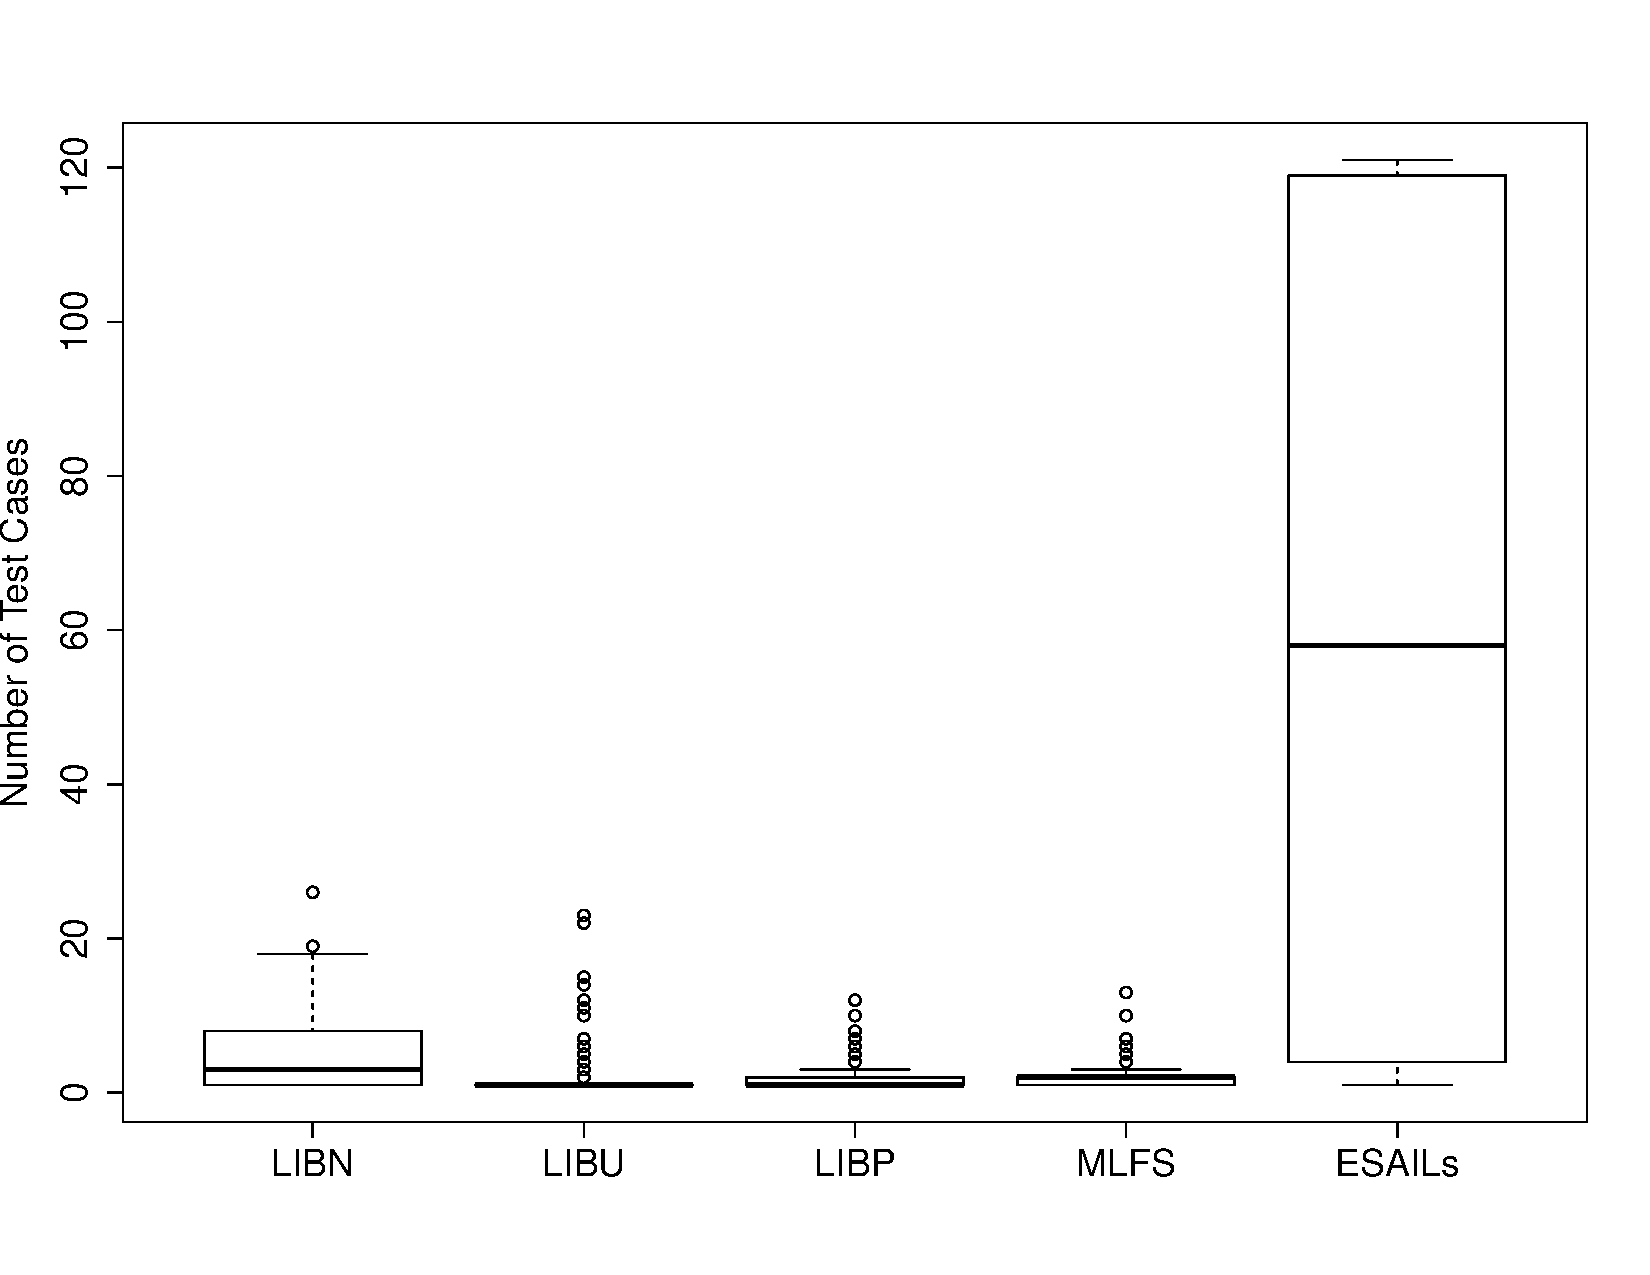
\includegraphics[width=0.8\columnwidth]{images/st_testcases}
\caption{Distribution of test cases exercising each statement.}
\label{fig:tastCaseDist}
\end{center}
\end{figure}

%> min(csp$V1)
%[1] 1
%> min(util$V1)
%[1] 1
%> min(param$V1)
%[1] 1
%> min(mlfs$V1)
%[1] 1
%> min(esail$V1)
%[1] 1
%> max(csp$V1)
%[1] 26
%> max(util$V1)
%[1] 23
%> max(param$V1)
%[1] 12
%> max(mlfs$V1)
%[1] 13
%> max(esail$V1)
%[1] 121
%> mean(csp$V1)
%[1] 4.493617
%> mean(util$V1)
%[1] 1.745416
%> mean(param$V1)
%[1] 2.760691
%> mean(mlfs$V1)
%[1] 2.524808
%> mean(esail$V1)
%[1] 60.96341
%> median(csp$V1)
%[1] 3
%> median(util$V1)
%[1] 1
%> median(param$V1)
%[1] 1
%> median(mlfs$V1)
%[1] 2
%> median(esail$V1)
%[1] 58
%                   [,csp] [,uti] [,para] [,mlf] [,esa]
%[lower whisker,]    1    1    1    1    1
%[lower hinge,]       1    1    1    1    4
%[median,]              3    1    1    2   58
%[upper hinge,]      8    1    2     2   119
%[upper whisker,]   18    1    3    3  121


To address some of our research questions, all the mutants must be executed against the test suite, which is not feasible for the case of \SAIL{}\emph{-CSW} due to its large size and test suite. For this reason, we have identified a subsystem of \SAIL{}\emph{-CSW} (hereafter, \emph{\SAIL{}}$_{S}$) that consists of a set of files, selected by \TWO engineers, that are representative of the different functionalities in \SAIL{}\emph{-CSW}: service/protocol layer functions, critical functions of the satellite implemented in high-level drivers, application layer functions.
Details about $\mathit{\SAIL{}}_{S}$ are reported in Table~\ref{table:caseStudies}.
% \FIXME{note that statement coverage is in line with the whole system.}


Except for \SAIL{}\emph{-CSW}, all subjects
are compiled to generate executables for the development environment OS (Linux); we rely on the Gnu Compiler Collection (GCC)  for Linux X86~\cite{GCC} versions 5.3 and 6.3 for \MLFS{}{} and ONE, respectively. \SAIL{}\emph{-CSW} is compiled with the
LEON/ERC32 RTEMS Cross Compilation System, which includes the GCC C/C++ compiler version 4.4.6 for  RTEMS-4.8 (Sparc architecture)~\cite{RTEMS}.

It is important to note that the technical and test suite characteristics described above are very common in embedded software across many industry domains and cyber-physical systems, thus suggesting our results can be generalizable beyond space software. 

% !TEX root =  ../Main.tex

\begin{table}[tb]
\caption{Descriptions of software components.}
\label{table:caseStudies} 
\scriptsize
\centering
\begin{tabular}{|
@{\hspace{1pt}}p{12mm}
@{\hspace{2pt}}|
@{\hspace{1pt}}>{\raggedleft\arraybackslash}p{8mm}@{\hspace{1pt}}|
@{\hspace{1pt}}>{\raggedleft\arraybackslash}p{18mm}@{\hspace{1pt}}|
@{\hspace{1pt}}>{\raggedleft\arraybackslash}p{20mm}@{\hspace{1pt}}|
@{\hspace{1pt}}>{\raggedleft\arraybackslash}p{24mm}@{\hspace{1pt}}|
p{20mm}|}
\hline
\textbf{Component}&\textbf{LOC}&\textbf{Test suite type}&\textbf{\# Test cases}&\textbf{Statements} \textbf{coverage}\\
\hline
ESAIL& 74155 & System& 384 & 90.38\% \\
ESAIL$_S$& 2235 & System& 384 & 95.36\%\\
LIBGSCSP& 9836 & Integration& 89 & 63.10\%\\
LIBPARAM& 3179 & Integration& 170 & 77.60\%\\
LIBUTIL& 10576 & Unit& 201 & 83.20\%\\
MLFS& 5402 & Unit& 4042 & 100.00\%\\
%MLFS$_V$& 5402 & 4042 & 100.00\%\\
\hline
\end{tabular}

\end{table}

% !TEX root =  ../Main.tex

\begin{table}[tb]
\caption{Generated and compiled mutants per component.}
\label{table:mutants} 
\scriptsize
\begin{tabular}{|
@{\hspace{1pt}}p{12mm}
@{\hspace{2pt}}|
>{\raggedleft\arraybackslash}p{8mm}@{\hspace{1pt}}|
>{\raggedleft\arraybackslash}p{12mm}@{\hspace{1pt}}|
>{\raggedleft\arraybackslash}p{12mm}@{\hspace{1pt}}|
>{\raggedleft\arraybackslash}p{12mm}@{\hspace{1pt}}|
>{\raggedleft\arraybackslash}p{12mm}|}
\hline
\textbf{Component}&\multicolumn{1}{c|}{\textbf{Mutants}}&\multicolumn{1}{c|}{\textbf{Mutants}}&\multicolumn{1}{c|}{\textbf{Mutants}}&\multicolumn{1}{c|}{\textbf{\% of}}&\multicolumn{1}{c|}{\textbf{Mutants}}\\
\textbf{}&\multicolumn{1}{c|}{\textbf{generated}}&\multicolumn{1}{c|}{\textbf{generation}}&\multicolumn{1}{c|}{\textbf{compiled}}&\multicolumn{1}{c|}{\textbf{compiled}}&\multicolumn{1}{c|}{\textbf{compilation}}\\ 
&&\textbf{time} \textbf{(sec)}&&\multicolumn{1}{c|}{\textbf{mutants}}&\multicolumn{1}{c|}{\textbf{time} \textbf{(sec)}}\\ 
\hline
ESAIL& 142763 & 182 &121848& 85.35\% & 151234\\
ESAIL$_S$& & & & &\\
LIBGSCSP& 8666 & 12 &7878&90.91\% & 11425\\
LIBPARAM& 7252 & 7 &6440&88.80\% & 9392\\
LIBUTIL& 22295 & 28 &20268&90.91\% & 30624\\
MLFS& 31526 & 20 &28069&89.03\% &3157\\
%MLFS$_V$& 31526 &T &28069&89.03\% &X\\
\hline
\textbf{Total*}& 212502 & 249 & 184503 &86.82\% &205832\\ 
\hline
\end{tabular}

* We ignore ESAIL$_S$ from the total counting because it is a subset of ESAIL.
\end{table}



\subsection{Setup}
\label{experimnt:setup}

%We should describe the operators used. Potentially could be the superset that is the union of all the operators used in the papers indicated above.
To perform the empirical evaluation, we have implemented the \APPR pipeline in a toolset that is available under the ESA Software Community Licence Permissive~\cite{ESAlicence} at the following URL \textbf{https://faqas.uni.lu/}.
%\footnote{Prior to acceptance, files are shared at {https://dropit.uni.lu/invitations?share=18629a285f6aceacd026}}.
For the implementation of mutation operators, we extended the SRCiror toolset~\cite{hariri2018srciror}.
In our analysis, we consider all the operators reported in Table 1.2 from D2.

Related studies~\cite{zhang2010operator,zhang2013operator} are performed by relying on mutation adequate test suites (i.e., test suites that kill all non-equivalent mutants). 
Such test suites are typically automatically generated using static analysis~\cite{papadakis2012mutation}.
%Since our subject artifacts, as it is common in cyber-physical domains, either require dedicated simulators or include network components, we cannot rely on static analysis to generate mutation adequate test suites. 
%We thus rely on the original test suites provided with the subjects. 
\JMR{3.13}{Since we cannot leverage static analysis to generate mutation adequate test suites (see Section~1.2.1.5 from D2), 
we rely on the original test suites provided with the subjects.}
As a result, to perform our study, we mutate only the statements that are covered by the considered test suites.

\CHANGED{For every subject, we generated mutants by executing the \APPR toolset on Linux OS running on a MacBook Pro with 2,3 GHz 8-Core Intel Core i9. 
Table~\ref{table:mutants} reports, for every subject, the total number of mutants that were generated, their generation time, the number of mutants successfully compiled, the proportion of compiled mutants with respect to the overall number of mutants generated, and the time required to compile mutants using one compiler optimization level only (i.e., the one originally selected by engineers for each subject).
%the default compiler optimization options of the subject.
The generation of mutants is fast, it takes at most {182} seconds on the largest subject (\SAIL{}\emph{-CSW}). On average, across subjects, it takes {11} milliseconds to generate a single mutant. 
The proportion of successfully compiled mutants is large (i.e., 86.82\% overall), though it varies from 85.35\% for \SAIL{}\emph{-CSW} to 90.91\% for \GCSP{} and \UTIL{}.
This proportion is in line with the ones reported in related work, though there is variation. For example, industrial systems 
%that likely contain complex instructions, 
have shown lower success rates (e.g., 81.13\% for safety-critical software components~\cite{Baker2013}) than open source, batch utilities (e.g., 96.30\% for Coreutils~\cite{hariri2016evaluating}).} \REVNOV{PTCR-17}{In the case of compiler warnings, we simply follow the policy configured for the case study. More precisely., in the case of ESAIl and MLFS all the warnings from the compiler lead to a compilation failure. In the case of GSL the compilation process proceeds.}
 
{As shown in Table~\ref{table:mutants}, the time required to compile all the mutants ranges from 3,157 to 151,234 seconds, for an average of 0.96 seconds required to compile a single mutant, across subjects. Because of our selective compilation strategy (see Section~1.2.7 from D2), the time required by our pipeline to compile a single mutant is significantly lower than the one required by state-of-the-art approaches, which is around 4.6 seconds per mutant, even when software components have a lower number of LOC %(i.e., 22,827 LOC)  
than our subjects~\cite{kintis2017detecting}.}

% {The last three columns of Table~\ref{table:mutants} present the number and percentage of mutants successfully compiled, along with the time required to compile all the mutants using the proposed incremental compilation process (Step 3 of \APPR). 
%In total, 86.82\% of the mutants generated among the four case study systems are successfully compiled. 
 



%According to previous research on mutant operator selection, we consider the superset, that is, the union of all the operators defined in the work by Offutt et al.~\cite{offutt1996experimental}, Andrews et al.~\cite{andrews2005mutation} and Kintis et al.~\cite{kintis2017detecting}. The superset consist of the AOR, LCR, ICR, ROR, SDL, UOI, and ABS.
%
%To asses our research questions with the different set of operators considered in the literature, we consider four interleaving subsets of the : the sufficient set (i.e., AOR, LCR, ICR, ROR, SDL, UOI, and ABS),
%the deletion set (i.e., SDL, AOD, LOD, ROD, BOD, and SOD), the extended sufficient set (i.e., all the operators in Table~\ref{table:operators}), and the statement deletion set (i.e., the SDL operator only).  



{To collect the data required to address research questions RQ2 to RQ8, for every subject and unique mutant generated by Step 3, we have executed all the test cases covering the mutated statement. Table~\ref{table:magnitude} provides, for every subject, the overall number of executed test cases and the total execution time required for our experiments. In total, the entire experiment took 1,912,662 minutes (31,878 hours or more than 1300 days). Test  execution time depends on the number of mutants, the number of executed test cases, and the test suite level (e.g., system test suites exercise more complex scenarios than unit or integration test suites).}  
%In our experiments, the execution times of the components tested with unit test suites \FIXME{have the same order of magnitude; indeed, they take between X and Y seconds to execute.}
%In the case of ESAIL, instead, \FIXME{....}}

\CHANGED{To be able to execute test cases for 31,878 hours, we performed our experiments using the HPC cluster of the University of Luxembourg~\cite{HPC}.
The HPC cluster consists of Intel Xeon E5-2680 v4 (2.4 GHz) nodes. To perform our experiments, we tested 100 mutants in parallel, each one on a dedicated node.}

% !TEX root =  ../Main.tex

\begin{table}[tb]
\caption{Experiments magnitude.}
\label{table:magnitude} 
\scriptsize
\centering
\begin{tabular}{|
@{\hspace{1pt}}p{12mm}
@{\hspace{2pt}}|
@{\hspace{1pt}}>{\raggedleft\arraybackslash}p{30mm}@{\hspace{1pt}}|
@{\hspace{1pt}}>{\raggedleft\arraybackslash}p{35mm}@{\hspace{1pt}}|
p{20mm}|}
\hline
\textbf{Case Study}&\textbf{Total test cases executed}&\textbf{Total execution time (minutes)}\\
\hline
%Fabrizio: after removing tests that do not cover the mutants, we should have lower numbers
ESAIL$_S$&  302\,158 & 1\,624\,336\\
LIBGSCSP&  771\,274 & 33\,756\\
LIBPARAM&  1\,094\,800 & 7\,205\\
LIBUTIL&  4\,481\,295 & 57\,732\\
MLFS&  170\,303\,452 & 189\,633\\
%MLFS$_V$& 5402 & 4042 & 100.00\%\\
\hline
\textbf{Total}&  176\,952\,979 & 1\,912\,662\\
\hline
\end{tabular}

\end{table}

In the following sections, we 
%analyze differences in results 
\JMR{3.11}{discuss statistical significance}
using a non-parametric Mann Whitney U-test (with $\alpha$ = 0.05)~\cite{Arcuri:practicalGuide:ICSE:2015}.  We discuss effect size based on Vargha and Delaney’s $A_{12}$ statistics, a non-parametric effect size measure~\cite{VDA,Arcuri:practicalGuide:ICSE:2015}. Based on $A_{12}$, effect size is considered small when $0.56 \le A_{12} < 0.64$, medium when $0.64 \le A_{12} < 0.71$, large when $A_{12} \ge 0.71$. Otherwise the compared samples are considered equivalent, that is to be drawn from the same population~\cite{VDA}.


% % !TEX root =  ../Main.tex

\newcommand{\op}{\mathit{op}}
\newcommand{\ArithmeticSet}{ \texttt{+}, \texttt{-}, \texttt{*}, \texttt{/}, \texttt{\%} }
\newcommand{\LogicalSet}{ \texttt{&&}, \texttt{||} }
\newcommand{\RelationalSet}{ \texttt{>}, \texttt{>=}, \texttt{<}, \texttt{<=}, \texttt{==}, \texttt{!=} }
\newcommand{\BitWiseSet}{ \texttt{\&}, \texttt{|}, \land }
\newcommand{\ShiftSet}{ \texttt{>>}, \texttt{<<} }


\begin{table}[h]
\caption{Implemented set of mutation operators.}
\label{table:operators} 
\centering
\scriptsize
\begin{tabular}{|@{}p{4mm}@{}|@{}p{2cm}@{\hspace{1pt}}|@{}p{11.1cm}@{}|}
\hline
&\textbf{Operator} & \textbf{Description$^{*}$} \\
\hline
\multirow{7}{*}{\rotatebox{90}{\emph{Sufficient Set}}}&ABS               & $\{(v, -v)\}$	\\
\cline{2-3}
&AOR               & $\{(\op_1, op_2) \,|\, \op_1, \op_2 \in \{ \ArithmeticSet \} \land \op_1 \neq \op_2 \} $       \\
&    			  & $\{(\op_1, \op_2) \,|\, \op_1, \op_2 \in \{\texttt{+=}, \texttt{-=}, \texttt{*=}, \texttt{/=}, \texttt{\%} \texttt{=}\} \land \op_1 \neq \op_2 \} $       \\
\cline{2-3}
&ICR               & $\{i, x) \,|\, x \in \{1, -1, 0, i + 1, i - 1, -i\}\}$           \\
\cline{2-3}
&LCR               & $\{(\op_1, \op_2) \,|\, \op_1, \op_2 \in \{ \texttt{\&\&}, || \} \land \op_1 \neq \op_2 \}$            \\
&				  & $\{(\op_1, \op_2) \,|\, \op_1, \op_2 \in \{ \texttt{\&=}, \texttt{|=}, \texttt{\&=}\} \land \op_1 \neq \op_2 \}$            \\
&				  & $\{(\op_1, \op_2) \,|\, \op_1, \op_2 \in \{ \texttt{\&}, \texttt{|}, \texttt{\&\&}\} \land \op_1 \neq \op_2 \}$            \\
\cline{2-3}
&ROR               & $\{(\op_1, \op_2) \,|\, \op_1, \op_2 \in \{ \RelationalSet \}\}$            \\
&				  & $\{ (e, !(e)) \,|\, e \in \{\texttt{if(e)}, \texttt{while(e)}\} \}$ \\
\cline{2-3}
&SDL               & $\{(s, \texttt{remove}(s))\}$            \\
\cline{2-3}
&UOI               & $\{ (v, \texttt{--}v), (v, v\texttt{--}), (v, \texttt{++}v), (v, v\texttt{++}) \}$            \\   
\hline
\hline
\multirow{5}{*}{\rotatebox{90}{\emph{OODL}}}&AOD               & $\{((t_1\,op\,t_2), t_1), ((t_1\,op\,t_2), t_2) \,|\, op \in \{ \ArithmeticSet \} $       \\ 
\cline{2-3}
&LOD               & $\{((t_1\,op\,t_2), t_1), ((t_1\,op\,t_2), t_2) \,|\, op \in \{  \} \}$       \\ 
\cline{2-3}
&ROD               & $\{((t_1\,op\,t_2), t_1), ((t_1\,op\,t_2), t_2) \,|\, op \in \{ \RelationalSet \} \}$       \\ 
\cline{2-3}
&BOD               & $\{((t_1\,op\,t_2), t_1), ((t_1\,op\,t_2), t_2) \,|\, op \in \{ \BitWiseSet \} \}$       \\ 
\cline{2-3}
&SOD               & $\{((t_1\,op\,t_2), t_1), ((t_1\,op\,t_2), t_2) \,|\, op \in \{ \ShiftSet \} \}$       \\ 
%\hline
%COR               & $\{(\op_1, \op_2) \,|\, \op_1, \op_2 \in \{ \texttt{\&\&}, \texttt{||}, \land \} \land \op_1 \neq \op_2 \}$            \\
\hline
\hline
\multirow{3}{*}{\rotatebox{90}{\emph{Other}}}&LVR			& $\{(l_1, l_2) \,|\, (l_1, l_2) \in \{(0,-1), (l_1,-l_1), (l_1, 0), (\mathit{true}, \mathit{false}), (\mathit{false}, \mathit{true})\}\}$\\
&&\\
&&\\
\hline
\end{tabular}

$^{*}$Each pair in parenthesis shows how a program element is modified by the mutation operator. Th eleft element of the pair is replaced with the right element. We follow standard syntax~\cite{kintis2018effective}. Program elements are literals ($l$), integer literals ($i$), boolean expressions ($e$), operators ($\op$), statements ($s$), variables ($v$), and terms ( $t_i$, which might be either variables or literals).
\end{table}

%To generate the mutants, we have extended the SRCIRor mutation testing tool~\cite{hariri2018srciror}. since the original version only implemented the set of operators AOR, LCR, ICR and ROR.

%For each subject of the study we generated mutants by applying the sufficient set of operators. We call this set of mutants complete mutants set.

%We executed the test suites of the case study systems against the complete mutants set. Test execution results let us compute the mutation score of the case study. For each case study, we kept track of the mutants killed by each test case.




%
%To address our research questions considering test suites with different mutation scores for the complete mutants set, for each case study, we derived subsets of the original test suites with different mutation scores. The test suites were randomly derived by randomly selecting test cases till a specific mutation score is reached. We consider test suites with the following mutation scores...

\subsection{RQ1}

% !TEX root =  ../Main.tex
\begin{table*}[htb]
\caption{RQ1. Proportion (\%) of Trivially-Equivalent and Trivially-Redundant Mutants Detected by Compiler Optimizations.}
\label{table:results:compilerOptimizations} 
\tiny
\centering
%\begin{tabular}{|
%p{11mm}|p{6mm}|p{10mm}|
%@{\hspace{2mm}}p{5mm}|p{5mm}|p{5mm}|p{5mm}|p{5mm}|p{5mm}|
%p{6mm}|p{6mm}|p{6mm}|p{6mm}|p{6mm}|p{6mm}|
%}
%\hline
%\textbf{Case} & \textbf{All} & \textbf{Compiled} & \multicolumn{6}{c|}{Equivalent} & \multicolumn{6}{c|}{Redundant} \\
%\textbf{Study}& & 
%&\textbf{O0}&\textbf{O1} & \textbf{O2} & \textbf{O3} & \textbf{Os} & \textbf{Of} 
%&\textbf{O0}&\textbf{O1} & \textbf{O2} & \textbf{O3} & \textbf{Os} & \textbf{Of}
%\\
%\hline
%ESAIL & 142763 & 121848 & 3029 & 8440 & 8520 & 8472 & 8634 & - & 14032 & 21011 & 21768 & 21613 & 21943 & - \\
% &  &  & 2.49  & 6.93  & 6.70  & 6.95  & 7.09  & - & 11.52  & 17.25  & 17.86  & 17.74  & 18.01  & - \\
%LIBUTIL & 22295 & 20268 & 394 & 1277 & 1233 & 1255 & 1247 & 1255 & 2093 & 3092 & 3320 & 3369 & 3383 & 3369 \\
% &  &  & 1.94  & 6.30  & 6.08  & 6.19  & 6.15  & 6.19  & 10.33  & 15.26  & 16.38  & 16.62  & 16.69  & 16.62  \\
%LIBPARAM & 7252 & 6440 & 151 & 428 & 423 & 425 & 436 & 425 & 909 & 1310 & 1346 & 1346 & 1348 & 1346 \\
% &  &  & 2.34  & 6.65  & 6.57  & 6.60  & 6.77  & 6.60 & 14.11  & 20.34  & 20.90  & 20.90  & 20.93  & 20.90  \\
%LIBGSCSP & 8666 & 7878 & 176 & 683 & 511 & 519 & 315 & 336 & 997 & 1756 & 1332 & 1528 & 1690 & 1672 \\
% &  &  & 2.23  & 8.67  & 6.49  & 6.59  & 4.00  & 4.27  & 12.66  & 22.29  & 16.91  & 19.40  & 21.45  & 21.22  \\
%MLFS & 31526 & 28069 & 115 & 230 & 281 & 282 & 307 & 293 & 2386 & 3244 & 3620 & 3628 & 3732 & 3895 \\
% &  &  & 0.41  & 0.82  & 1.00  & 1.00  & 1.09  & 1.04  & 8.50  & 11.55  & 12.90  & 12.93  & 13.30  & 13.88  \\
%\hline
%\textbf{Total}  & 212502 & 184503 & 3773 & 10559 & 10963 & 10557 & 11211 & 2096 & 20479 & 30414 & 31568 & 31800 & 31867 & 10458\\
%&  &  & 2.04  & 5.72  & 5.94  & 5.72  & 6.08  & 1.14  & 11.10  & 16.48  & 17.11  & 17.24  & 17.27  & 5.67  \\
%\hline
%
%\end{tabular}

\begin{tabular}{|
p{11mm}|
@{\hspace{1pt}} >{\raggedleft\arraybackslash}p{9mm}@{\hspace{1pt}}|
@{\hspace{1pt}}>{\raggedleft\arraybackslash}p{10mm}@{\hspace{1pt}}|
@{\hspace{1pt}}>{\raggedleft\arraybackslash}p{8mm}@{\hspace{1pt}}|
>{\raggedleft\arraybackslash}p{5mm}@{\hspace{1pt}}|
>{\raggedleft\arraybackslash}p{8mm}@{\hspace{1pt}}|
 >{\raggedleft\arraybackslash}p{5mm}@{\hspace{1pt}}|
 >{\raggedleft\arraybackslash}p{5mm}@{\hspace{1pt}}|
 >{\raggedleft\arraybackslash}p{5mm}@{\hspace{1pt}}|
 >{\raggedleft\arraybackslash}p{5mm}@{\hspace{1pt}}|
>{\raggedleft\arraybackslash}p{7mm}@{\hspace{1pt}}|
@{\hspace{1pt}} >{\raggedleft\arraybackslash}p{10mm}@{\hspace{1pt}}|
@{\hspace{1pt}} >{\raggedleft\arraybackslash}p{8mm}@{\hspace{1pt}}|
 >{\raggedleft\arraybackslash}p{8mm}@{\hspace{1pt}}|
 >{\raggedleft\arraybackslash}p{6mm}@{\hspace{1pt}}|
 >{\raggedleft\arraybackslash}p{6mm}@{\hspace{1pt}}|
 >{\raggedleft\arraybackslash}p{6mm}@{\hspace{1pt}}|
 >{\raggedleft\arraybackslash}p{6mm}@{\hspace{1pt}}|
 >{\raggedleft\arraybackslash}p{6mm}@{\hspace{1pt}}|
}







\hline
\textbf{Case} & \multicolumn{9}{c|}{\textbf{Equivalent}} & \multicolumn{9}{c|}{\textbf{Redundant}} \\
\textbf{Study}
&\textbf{All}&\textbf{Overall}\textbf{\%}&\textbf{-O0-3}&\textbf{-O0}&\textbf{-O1} & \textbf{-O2} & \textbf{-O3} & \textbf{-Os} & \textbf{-Of} 
&\textbf{All}&\textbf{Overall}\textbf{\%}&\textbf{-O0-3}&\textbf{-O0}&\textbf{-O1} & \textbf{-O2} & \textbf{-O3} & \textbf{-Os} & \textbf{-Of}
\\
\hline
ESAIL &8861&7.27 &7.13&34.18 &95.25 &96.15 &95.61 &97.44 &-&35133&28.83&27.74&39.94 &59.80 &61.96 &61.52 &62.46 &-\\
LIBUTIL &1366&6,74 &6.65&28.84 &93.48 &90.26 &91.87 &91.29 &91.87 &4392&21.67&21.26&47.65 &70.40 &75.59 &76.71 &77.03 &76.71 \\
LIBPARAM &450& 6.99 &6.89&33.56 &95.11 &94.00 &94.44 &96.89 &94.44 &2076&32.24&31.44&43.79 &63.10 &64.84 &64.84 &64.93 &64.84 \\
LIBGSCSP &701&8.90 &8.90&25.11 &97.43 &72.90 &74.04 &44.94 &47.93 &2655&33.70&27.63&37.55 &66.14 &50.17 &57.55 &63.65 &62.98 \\
MLFS &361 &1.29 &1.04&31.86 &63.71 &77.84 &78.12 &85.04 &81.16 &6356&22.64&20.13&37.54 &51.04 &56.95 &57.08 &58.72 &61.28 \\
\hline
\textbf{Total}  &11739&6.36 &6.22&32.14 &89.95 &93.39 &89.93 &95.50 &17.86 &50612&27.43&25.99&40.46 &60.09 &62.37 &62.83 &62.96 &20.66 \\
\hline

\end{tabular}


\end{table*}

\begin{table*}[htb]
\caption{RQ1.  Proportion (\%) of Univocal-Trivially-Equivalent and Univocal-Trivially-Redundant Mutants Detected by Compiler Optimizations.}
\label{table:results:compilerOptimizationsUnivocal} 
\tiny
%\centering
%\begin{tabular}{|
%p{11mm}|p{6mm}|p{10mm}|
%@{\hspace{2mm}}p{6mm}|p{6mm}|p{6mm}|p{6mm}|p{6mm}|p{6mm}|
%p{6mm}|p{6mm}|p{6mm}|p{6mm}|p{6mm}|p{6mm}|
%}
%\hline
%\textbf{Case} & \textbf{All} & \textbf{Compiled} & \multicolumn{6}{c|}{Univocal-Equivalent} & \multicolumn{6}{c|}{Univocal-Redundant} \\
%\textbf{Study}& & 
%&\textbf{O0}&\textbf{O1} & \textbf{O2} & \textbf{O3} & \textbf{Os} & \textbf{Of} 
%&\textbf{O0}&\textbf{O1} & \textbf{O2} & \textbf{O3} & \textbf{Os} & \textbf{Of}
%\\
%\hline
%
%ESAIL & 142763 & 121848 & 0 & 11 & 2 & 47 & 177 & - & 516 & 999 & 1033 & 1175 & 1334 & - \\
%  & & & 0.000  & 0.009  & 0.001  & 0.039  & 0.145  & - & 0.423  & 0.819  & 0.850  & 0.964  & 1.094  & - \\
%LIBUTIL & 22295 & 20268 & 1 & 74 & 2 & 0 & 19 & 0 & 818 & 48 & 4 & 0 & 79 & 4\\
% & & & 0.005  & 0.365  & 0.010  & 0.000  & 0.094  & 0.000  & 4.036  & 0.237  & 0.019  & 0.000  & 0.389  & 0.019  \\
%LIBPARAM & 7252 & 6440 & 0 & 5 & 0 & 0 & 6 & 0 & 20 & 55 & 54 & 0 & 51 & 0\\
% & & & 0.000  & 0.078  & 0.000  & 0.000  & 0.093  & 0.000   & 0.311  & 0.854  & 0.839  & 0.000  & 0.791  & 0.000  \\
%LIBGSCSP & 8666 & 7878 & 0 & 0 & 7 & 0 & 23 & 0 & 1 & 58 & 89 & 0 & 98 & 0\\
% & & & 0.000  & 0.000  & 0.089  & 0.000  & 0.292  & 0.000  & 0.013  & 0.736  & 1.130  & 0.000  & 1.244  & 0.000  \\
%MLFS & 31526 & 28069 & 0 & 6 & 0 & 0 & 39 & 20 & 6 & 60 & 340 & 2 & 443 & 256\\
% & & & 0.000  & 0.021  & 0.000  & 0.000  & 0.139  & 0.071  & 0.021  & 0.214  & 1.211  & 0.007  & 1.578  & 0.912  \\
%\hline
%\textbf{Total}  & 212502 & 184503 & 1 & 96 & 11 & 47 & 264 & 20 & 1046 & 2113 & 529 & 277 & 3114 & 318 \\
% & & & 0.001  & 0.052  & 0.001  & 0.025  & 0.143  & 0.011  & 0.567  & 1.145  & 0.287  & 0.150  & 1.689  & 0.172  \\
%\hline
%
%\end{tabular}

\begin{tabular}{|
p{11mm}|
@{\hspace{1pt}} >{\raggedleft\arraybackslash}p{9mm}@{\hspace{1pt}}|
@{\hspace{1pt}}>{\raggedleft\arraybackslash}p{19mm}@{\hspace{1pt}}|
>{\raggedleft\arraybackslash}p{5mm}@{\hspace{1pt}}|
>{\raggedleft\arraybackslash}p{8mm}@{\hspace{1pt}}|
 >{\raggedleft\arraybackslash}p{5mm}@{\hspace{1pt}}|
 >{\raggedleft\arraybackslash}p{5mm}@{\hspace{1pt}}|
 >{\raggedleft\arraybackslash}p{5mm}@{\hspace{1pt}}|
 >{\raggedleft\arraybackslash}p{5mm}@{\hspace{1pt}}|
>{\raggedleft\arraybackslash}p{7mm}@{\hspace{1pt}}|
@{\hspace{1pt}} >{\raggedleft\arraybackslash}p{19mm}@{\hspace{1pt}}|
 >{\raggedleft\arraybackslash}p{8mm}@{\hspace{1pt}}|
 >{\raggedleft\arraybackslash}p{6mm}@{\hspace{1pt}}|
 >{\raggedleft\arraybackslash}p{6mm}@{\hspace{1pt}}|
 >{\raggedleft\arraybackslash}p{6mm}@{\hspace{1pt}}|
 >{\raggedleft\arraybackslash}p{6mm}@{\hspace{1pt}}|
 >{\raggedleft\arraybackslash}p{6mm}@{\hspace{1pt}}|
}







\hline
\textbf{Case} & \multicolumn{8}{c|}{\textbf{Univocal-Equivalent}} & \multicolumn{8}{c|}{\textbf{Univocal-Redundant}} \\
\textbf{Study}
&\textbf{All}&\textbf{\%} \textbf{of} \textbf{Equivalent}&\textbf{-O0}&\textbf{-O1} & \textbf{-O2} & \textbf{-O3} & \textbf{-Os} & \textbf{-Of} 
&\textbf{All}&\textbf{\%} \textbf{of} \textbf{Redundant}&\textbf{-O0}&\textbf{-O1} & \textbf{-O2} & \textbf{-O3} & \textbf{-Os} & \textbf{-Of}
\\
\hline
ESAIL &237& 2.67&0.00 &4.64 &0.84 &19.83 &\textbf{74.68} &0.00 &5057&14.39&10.20 &19.75 &20.43 &23.24 &\textbf{26.38} &0.00  \\
LIBUTIL &96& 7.03&1.04 &77.08 &2.08 &0.00 &\textbf{19.79} &0.00 &953& 21.70&\textbf{85.83} &5.04 &0.42 &0.00 &8.29 &0.42  \\
LIBPARAM &11 & 2.44&0.00 &45.45 &0.00 &0.00 &\textbf{54.55} &0.00 &180& 8.67&11.11 &\textbf{30.56} &30.00 &0.00 &28.33 &0.00  \\
LIBGSCSP &112 & 15.98&25.11 &\textbf{97.43} &72.90 &74.04 &44.94 &47.93 &429& 16.16&37.55 &\textbf{66.14} &50.17 &57.55 &63.65 &62.98  \\
MLFS &65& 18.01&0.00 &9.23 &0.00 &0.00 &60.00 &\textbf{30.77} &1107& 17.42&0.54 &5.42 &30.71 &0.18 &\textbf{40.02} &23.13 \\
\hline
\textbf{Total}  &521& 4.44&0.19 &18.43 &2.11 &9.02 &\textbf{50.67} &3.84 &7726& 15.27&13.54 &27.35 &6.85 &3.59 &\textbf{40.31} &4.12 \\
\hline

\end{tabular}


\end{table*}


% \begin{table*}[htb]
% \caption{RQ1. Equivalent and Redundant Mutants Detected by Compiler Optimizations.}
% \label{table:results:compilerOptimizations} 
% \tiny
% \begin{tabular}{|
% p{7mm}|p{5mm}|p{7mm}|
% @{\hspace{1mm}}p{4mm}|p{2mm}|p{2mm}|p{2mm}|p{2mm}|p{2mm}|p{2mm}|
% p{2mm}|p{2mm}|p{2mm}|p{2mm}|p{2mm}|p{2mm}|
% p{2mm}|p{2mm}|p{2mm}|p{2mm}|p{2mm}|p{2mm}|
% p{2mm}|p{2mm}|p{2mm}|p{2mm}|p{2mm}|p{2mm}|
% }
% \hline
% \textbf{Case} & \textbf{All} & \textbf{Compiled} & \multicolumn{6}{c|}{Equivalent} & \multicolumn{6}{c|}{Redundant} 
% & \multicolumn{6}{c|}{Univocal-Equivalent}  & \multicolumn{6}{c|}{Univocal-Redundant} \\
% \textbf{Study}&&
% &\textbf{O0}&\textbf{O1} & \textbf{O2} & \textbf{O3} & \textbf{Os} & \textbf{Of} 
% &\textbf{O0}&\textbf{O1} & \textbf{O2} & \textbf{O3} & \textbf{Os} & \textbf{Of}
% &\textbf{O0}&\textbf{O1} & \textbf{O2} & \textbf{O3} & \textbf{Os} & \textbf{Of} 
% &\textbf{O0}&\textbf{O1} & \textbf{O2} & \textbf{O3} & \textbf{Os} & \textbf{Of}
% \\
% ESAIL & 142763 & 121848 & 3029 & 8440 & 8520 & 8472 & 8634 &  & 14032 & 21013 & 21768 & 21613 & 21944 & & 0 & 11 & 2 & 47 & 177 & & 1032 & 1923 & 90 & 240 & 2463 & \\
%  &  &  & 2.49  & 6.93  & 6.70  & 6.95  & 7.09  &  & 11.52  & 17.25  & 17.86  & 17.74  & 18.01  & & 0.00  & 9e-03  & 1.6e-03  & 0.04  & 0.15  &  & 0.85  & 1.58  & 0.07   & 0.2  & 2.02  & \\
% LIBUTIL & 22295 & 20268 & 394 & 1277 & 1233 & 1255 & 1247 & 1255 & 2093 & 3092 & 3319 & 3364 & 3381 & 3368 & 1 & 74 & 2 & 0 & 19 & 0 & 7 & 56 & 7 & 35 & 87 & 62\\
% LIBPARAM & 7252 & 6440 & 151 & 428 & 423 & 425 & 436 & 425 & 909 & 1309 & 1346 & 1346 & 1347 & 1346 & 0 & 5 & 0 & 0 & 6 & 0 & 0 & 16 & 3 & 0 & 23 & 0\\
% LIBGSCSP & 8666 & 7878 & 84 & 184 & 506 & 123 & 587 & 123 & 1059 & 1756 & 1515 & 1849 & 1463 & 1849 & 0 & 0 & 7 & 0 & 23 & 0 & 1 & 58 & 89 & 0 & 98 & 0\\
% MLFS & 31526 & 28069 & 115 & 230 & 281 & 282 & 307 & 293 & 2386 & 3244 & 3620 & 3628 & 3732 & 3895 & 0 & 6 & 0 & 0 & 39 & 20 & 6 & 60 & 340 & 2 & 443 & 256\\
% \hline
% \textbf{Total}  & 212502 & 184503 & 3773 & 10559 & 10963 & 10557 & 11211 & 2096 & 20479 & 30414 & 31568 & 31800 & 31867 & 10458 & 1 & 96 & 11 & 47 & 264 & 20 & 1046 & 2113 & 529 & 277 & 3114 & 318 \\

% %\hline
% %ES\\
% %\hline
% \end{tabular}

% \end{table*}

\begin{table*}[htb]
\caption{RQ1.  Proportion (\%) of Trivially Equivalent/Redundant Mutants Detected per Mutation Operator.}
\label{table:results:compilerOptimizationsProportionOperators} 
\scriptsize
\begin{tabular}{|
p{11mm}|
>{\raggedleft\arraybackslash}p{5mm}@{\hspace{1pt}}|
@{\hspace{1pt}}>{\raggedleft\arraybackslash}p{5mm}@{\hspace{1pt}}|
@{\hspace{1pt}} >{\raggedleft\arraybackslash}p{5mm}@{\hspace{1pt}}|
@{\hspace{1pt}} >{\raggedleft\arraybackslash}p{5mm}@{\hspace{1pt}}|
@{\hspace{1pt}} >{\raggedleft\arraybackslash}p{5mm}@{\hspace{1pt}}|
@{\hspace{1pt}} >{\raggedleft\arraybackslash}p{5mm}@{\hspace{1pt}}|
@{\hspace{1pt}} >{\raggedleft\arraybackslash}p{5mm}@{\hspace{1pt}}|
@{\hspace{1pt}} >{\raggedleft\arraybackslash}p{5mm}@{\hspace{1pt}}|
@{\hspace{1pt}} >{\raggedleft\arraybackslash}p{5mm}@{\hspace{1pt}}|
@{\hspace{1pt}} >{\raggedleft\arraybackslash}p{5mm}@{\hspace{1pt}}|
@{\hspace{1pt}} >{\raggedleft\arraybackslash}p{5mm}@{\hspace{1pt}}|
@{\hspace{1pt}} >{\raggedleft\arraybackslash}p{5mm}@{\hspace{1pt}}|
@{\hspace{1pt}} >{\raggedleft\arraybackslash}p{5mm}@{\hspace{1pt}}|
 >{\raggedleft\arraybackslash}p{5mm}@{\hspace{1pt}}|
@{\hspace{1pt}}>{\raggedleft\arraybackslash}p{5mm}@{\hspace{1pt}}|
@{\hspace{1pt}} >{\raggedleft\arraybackslash}p{5mm}@{\hspace{1pt}}|
@{\hspace{1pt}} >{\raggedleft\arraybackslash}p{5mm}@{\hspace{1pt}}|
@{\hspace{1pt}} >{\raggedleft\arraybackslash}p{5mm}@{\hspace{1pt}}|
@{\hspace{1pt}} >{\raggedleft\arraybackslash}p{5mm}@{\hspace{1pt}}|
@{\hspace{1pt}} >{\raggedleft\arraybackslash}p{5mm}@{\hspace{1pt}}|
@{\hspace{1pt}} >{\raggedleft\arraybackslash}p{5mm}@{\hspace{1pt}}|
@{\hspace{1pt}} >{\raggedleft\arraybackslash}p{5mm}@{\hspace{1pt}}|
@{\hspace{1pt}} >{\raggedleft\arraybackslash}p{5mm}@{\hspace{1pt}}|
@{\hspace{1pt}} >{\raggedleft\arraybackslash}p{5mm}@{\hspace{1pt}}|
@{\hspace{1pt}} >{\raggedleft\arraybackslash}p{5mm}@{\hspace{1pt}}|
@{\hspace{1pt}} >{\raggedleft\arraybackslash}p{5mm}@{\hspace{1pt}}|
}

\hline
\textbf{Case}& \multicolumn{13}{c|}{\textbf{Trivially Equivalent}} &\multicolumn{13}{c|}{\textbf{Trivially Redundant}}\\
\textbf{Study}&
\textbf{ABS}&	\textbf{AOR}&	\textbf{ICR}&	\textbf{LCR}&	\textbf{ROR}&	\textbf{SDL}&	\textbf{UOI}&	\textbf{AOD}&	\textbf{LOD}&	\textbf{ROD}&	\textbf{BOD}&	\textbf{SOD}&	\textbf{LVR}&
\textbf{ABS}&	\textbf{AOR}&	\textbf{ICR}&	\textbf{LCR}&	\textbf{ROR}&	\textbf{SDL}&	\textbf{UOI}&	\textbf{AOD}&	\textbf{LOD}&	\textbf{ROD}&	\textbf{BOD}&	\textbf{SOD}&	\textbf{LVR}\\
\hline
ESAIL&3.65&1.85&6.74&2.09&18.00&1.60&52.34&1.53&0.05&7.64&3.42&0.51&0.59&1.52&6.20&18.79&1.05&23.89&8.04&20.23&4.83&1.06&8.86&2.20&1.96&1.39\\
LIBUTIL&6.66&0.07&3.95&1.24&15.96&7.91&58.86&0.00&0.37&3.81&0.95&0.00&0.22&0.34&7.38&15.64&0.87&30.35&12.61&13.52&1.66&2.66&12.77&0.89&0.52&0.77\\
LIBPARAM&8.89&0.00&0.00&0.22&25.56&6.22&55.33&0.00&0.00&3.56&0.22&0.00&0.00&0.96&3.47&7.95&1.01&36.71&13.58&12.52&1.49&2.46&18.45&0.92&0.00&0.48\\
LIBGSCSP&8.84&0.00&2.28&1.14&17.40&3.14&56.35&0.00&0.14&9.84&0.86&0.00&0.00&2.11&2.37&10.77&1.24&31.45&9.04&23.92&1.69&1.36&13.48&1.58&0.79&0.19\\
MLFS&6.37&0.55&11.63&0.28&27.98&2.77&39.61&0.00&0.00&9.42&1.39&0.00&0.00&5.03&10.12&25.36&0.87&23.77&4.14&6.73&8.51&0.88&9.44&2.33&1.90&0.91\\
\hline
\textbf{Total}&4.59&1.42&6.04&1.81&18.32&2.64&\textbf{53.06}&1.16&0.09&7.22&2.79&0.38&0.47&1.87&6.48&18.47&1.02&25.36&8.23&\textbf{17.83}&4.72&1.25&9.91&2.02&1.68&1.17\\
\hline
\end{tabular}


\end{table*}
% !TEX root =  ../Main.tex

\begin{table}[h]
\caption{RQ1. Compilation Time Required by Compiler Optimization Techniques.}
\label{table:results:compilerOptimizationsTime} 
\tiny
\centering
\begin{tabular}{|
@{\hspace{1pt}}p{11mm}|
@{\hspace{1pt}}>{\raggedleft\arraybackslash}p{7mm}@{\hspace{1pt}}|
>{\raggedleft\arraybackslash}p{7mm}@{\hspace{1pt}}|
>{\raggedleft\arraybackslash}p{7mm}@{\hspace{1pt}}|
>{\raggedleft\arraybackslash}p{7mm}@{\hspace{1pt}}|
>{\raggedleft\arraybackslash}p{7mm}@{\hspace{1pt}}|
>{\raggedleft\arraybackslash}p{7mm}@{\hspace{1pt}}|
 >{\raggedleft\arraybackslash}p{16mm}@{\hspace{1pt}}|
}
\hline
\textbf{Case} & 
\multicolumn{7}{c|}{\textbf{Time required to compile all the mutants(sec)}}\\
\textbf{Study}&
\textbf{O0}&\textbf{O1} & \textbf{O2} & \textbf{O3} & \textbf{Os} & \textbf{Of}
&\textbf{All O* (hours)} 
\\
\hline
ESAIL & 135455 & 132528 & 149088 & 145620 & 151234 & N/A&198\\
LIBUTIL & 25228 & 26914 & 28564 & 30624 & 26845 & 29583 &47\\
LIBPARAM & 9036 & 9246 & 9352 & 9392 & 8794 & 9442 &16\\
LIBGSCSP & 11053 & 11256 & 11079 & 11425 & 10299 & 11424 &18\\
MLFS & 2176 & 2509 & 3157 & 3167 & 3052 & 3164 &5\\
\hline
\textbf{Total}&182948	&182453	&201240	&200228	&200224	&53613 & 284\\
\hline
\end{tabular}

\end{table}

\paragraph{Design and measurements}

RQ1 aims to determine the cost savings provided by 
trivial compiler optimization techniques~\cite{papadakis2015trivial,kintis2017detecting}. To do so, we assess the number of equivalent and duplicate mutants discarded by these techniques and the additional costs introduced by the augmented compilation process. Since the mutants detected by these techniques 
are a subset of 
the overall set of equivalent and duplicate mutants, we refer to them as \INDEX{trivially equivalent} and \INDEX{trivially duplicate} mutants.

For every subject, we compile every mutant six times, each time with a different optimization level enabled. We consider all the available \INDEX{optimization levels} for the GCC compiler, which are \emph{-O0}, \emph{-O1}, \emph{-O2}, \emph{-O3}, \emph{-Os},
% (O2 it includes all O2 optimizations except those increasing executable size), 
and \emph{-Ofast}~\cite{GCCopt}. Level \emph{-O0} indicates that no optimization is applied. Levels \emph{-O1}, \emph{-O2}, \emph{-O3}, and \emph{-Ofast}, in this order, enable an increasing number of optimization options (e.g., level \emph{-Ofast} includes all the optimizations of level \emph{-O3} plus two additional ones, which are \emph{-ffast-math} and \emph{-fallow-store-data-races}). Level \emph{-Os} enables all \emph{-O2} optimizations except those that increase code size. This is the first reported experiment including options \emph{-Os} and \emph{-Ofast} in such an analysis.
 

To identify the most effective compiler optimization level, we consider the percentage of trivially equivalent and trivially duplicate mutants they detect. Also, to discuss how complementary different optimization levels  are and, therefore, whether they should be combined, we report the number of mutants identified as equivalent and duplicate by each compiler optimization only (hereafter called \INDEX{univocal-trivially-equivalent mutants} and \INDEX{univocal-trivially-duplicate mutants}). 

\CHANGED{To further assess the different optimization levels, we analyze the distribution of trivially equivalent and duplicate mutants across the different mutation operators considered in our study.}
% and, furthermore, we manually inspect a randomly selected sample of univocal-equivalent and univocal-duplicate mutants.} 
Last, we compare our results with the ones reported in related work~\cite{papadakis2015trivial}.

\CHANGED{By default, subjects are compiled with  different compiler optimization options, \emph{-Os} for \SAIL{}\emph{-CSW}, \emph{-O2} for \MLFS{}{}, \emph{-O3} for \GCSP{}, \PARAM{}, and \UTIL{}.}
To estimate the costs entailed by the augmented compilation process, we collect, for every subject, the time required for compiling all their mutants with each of the five optimization levels enabled. To compile mutants, we rely on the optimized compilation process implemented in Step 3 of \APPR (see Section~1.2.7 from D2).



\paragraph{Results}

Table~\ref{table:results:compilerOptimizations} provides the results concerning the detection of trivially equivalent and trivially duplicate mutants. We report the total number of such mutants detected for each subject (column \emph{All}), their percentage with respect to the set of mutants successfully compiled (column \emph{Overall \%}), and the percentages obtained with the options included in related work (i.e., by discarding the equivalent and duplicate mutants detected by \emph{-O0}, \emph{-O1}, \emph{-O2}, and \emph{-O3}, reported in column \emph{-O0-3}). 
 The proportion of trivially equivalent mutants detected with optimization levels O0-O3 (6.22\%) is in line with related work~\cite{papadakis2015trivial} (7\%) and the range observed for the different subjects (i.e., 1.04\% to 8.90\%) largely overlaps with the range observed in related work (2\%-10\%). 
 %However, the difference in means with related work is statistically significant and effect size is medium. 
 %Such results can be explained by the fact that, in our context, domain-specific functionalities and code adhering to coding standards are less likely to lead to the generation of trivially equivalent mutants (i.e., any small change in the code tends to impact software behaviour).
 For trivially duplicate mutants, instead, we observe a slightly larger set of duplicate mutants when compared to related work. Optimization levels O0-O3 determine that 25.99\% of the mutants are trivially duplicate, while in related work the average is around 21\%. Finally,  
 optimization levels \emph{-Os} and \emph{-Of} enable the detection of additional trivially equivalent and duplicate mutants, thus leading to an average of \JMR{3.12}{6.36\% and 27.43\% of the mutants being discarded, respectively (see column \emph{Overall \%})}. In particular, \textbf{we observe that the optimization level \emph{-Os}, not evaluated by related work, is the most effective}. Our results confirm the effectiveness of compiler optimizations for removing a significant percentage of equivalent and duplicate mutants.
 
Table~\ref{table:results:compilerOptimizationsUnivocal} provides additional details about the trivially equivalent and duplicate mutants univocally detected by the different optimization options. In total, 4.44\% and 3.34\% of these mutants are univocally detected  by one optimization level (see columns \emph{\% of Equivalent} and \emph{\% of Duplicate}); moreover, since all optimization options contribute to the univocal detection of equivalent and redundant mutants, \textbf{it is preferable to rely on all the available compiler optimization options}. 
\UPDATE{Overall, the most effective optimization option is \emph{-Os}, which detects 50.67\% and 46.34\% of univocal-equivalent and univocal-duplicate mutants, respectively. It is followed by \emph{-O1}, detecting 18.43\% and 10.82\% of such mutants, respectively}. These results suggest that, when the number of compilation runs must be limited, then \emph{-Os} and \emph{-O1} should be prioritized over the other options. This is interesting since \textbf{stronger optimization levels such as \emph{-Ofast} and \emph{-O3} do not contribute more than \emph{-Os} to the detection trivially equivalent and duplicate mutants}. Surprisingly, the optimization level \emph{-O0}, which does not enable any compiler optimization option, can detect trivially equivalent and trivially redundant mutants not detected by other optimization levels. However, this seems to highly depend on the code surrounding the mutated statement. 
\JMR{3.14}{For example, in one \UTIL mutant the optimization level \emph{-O0} detected that \texttt{if ( ptr )} is equivalent to \texttt{if( ptr > NULL )}, with \texttt{ptr} being a pointer, which was not detected with other optimization levels; however, the same instructions are detected as equivalent by other optimization levels when they belong to other functions (i.e., when the code surrounding them is different than the one appearing in the \UTIL mutant).}


To enable further comparison with related work~\cite{kintis2017detecting},
in Table~\ref{table:results:compilerOptimizationsProportionOperators}, we report the proportion of trivially equivalent and  duplicate mutants per mutation operator. The mutation operator causing the largest number of trivially equivalent mutants is UOI (e.g., 
it applies a post-increment operator to the last use of a variable),
%it post-increments the last use of a variable), 
followed by ROR, 
%(e.g., \FIXME{it ... }), 
ROD, 
%(e.g., \FIXME{it ...}), 
and ICR. 
%(e.g., because \FIXME{it ...}). 
Related studies are conducted with a smaller set of operators~\cite{kintis2017detecting}; however, the operators causing the largest numbers of trivially equivalent and duplicate mutants are the same. The main difference with related work~\cite{kintis2017detecting} concerns the ABS operator, which leads to a small set of equivalent mutants in our case, the main reason being that we rely on a definition of the ABS operator that minimizes the number of equivalent mutants by simply inverting the sign of the value instead of using the \emph{abs} function~\cite{Kintis2018}. Indeed, in functions with a positive integer domain, the replacement of a value with its absolute value trivially leads to equivalent mutants. Except for the ABS operator, \textbf{our study confirms the ranking observed in related work} despite different showing proportions. In addition, our results show that \textbf{the nature of the software affects the distribution of equivalent and duplicate mutants across operators}. Indeed, \MLFS{}{}, which focuses on mathematical functions, includes larger proportions of equivalent and duplicate mutants caused by ICR and AOR. In \PARAM{}, which does not deal with mathematical functions, the number of equivalent and duplicate mutants caused by these operators is much smaller. Finally, we notice that the \textbf{SDL and OODL operators lead to a minimal set of trivially equivalent and duplicate mutants, except for ROD}.

% !TEX root =  ../Main.tex

\begin{table*}[htb]
\caption{RQ1.  Proportion (\%) of Trivially Equivalent/Duplicate Mutants Detected per Mutation Operator.}
\label{table:results:compilerOptimizationsProportionOperators} 
\scriptsize
\centering
\begin{tabular}{|
@{\hspace{1pt}}p{9mm}|
@{\hspace{1pt}}>{\raggedleft\arraybackslash}p{5mm}@{\hspace{1pt}}|
@{\hspace{1pt}}>{\raggedleft\arraybackslash}p{5mm}@{\hspace{1pt}}|
@{\hspace{1pt}} >{\raggedleft\arraybackslash}p{5mm}@{\hspace{1pt}}|
@{\hspace{1pt}} >{\raggedleft\arraybackslash}p{5mm}@{\hspace{1pt}}|
@{\hspace{1pt}} >{\raggedleft\arraybackslash}p{5mm}@{\hspace{1pt}}|
@{\hspace{1pt}} >{\raggedleft\arraybackslash}p{5mm}@{\hspace{1pt}}|
@{\hspace{1pt}} >{\raggedleft\arraybackslash}p{5mm}@{\hspace{1pt}}|
@{\hspace{1pt}} >{\raggedleft\arraybackslash}p{5mm}@{\hspace{1pt}}|
@{\hspace{1pt}} >{\raggedleft\arraybackslash}p{5mm}@{\hspace{1pt}}|
@{\hspace{1pt}} >{\raggedleft\arraybackslash}p{5mm}@{\hspace{1pt}}|
@{\hspace{1pt}} >{\raggedleft\arraybackslash}p{5mm}@{\hspace{1pt}}|
@{\hspace{1pt}} >{\raggedleft\arraybackslash}p{5mm}@{\hspace{1pt}}|
@{\hspace{1pt}} >{\raggedleft\arraybackslash}p{5mm}@{\hspace{1pt}}|
 >{\raggedleft\arraybackslash}p{5mm}@{\hspace{1pt}}|
@{\hspace{1pt}}>{\raggedleft\arraybackslash}p{5mm}@{\hspace{1pt}}|
@{\hspace{1pt}} >{\raggedleft\arraybackslash}p{5mm}@{\hspace{1pt}}|
@{\hspace{1pt}} >{\raggedleft\arraybackslash}p{5mm}@{\hspace{1pt}}|
@{\hspace{1pt}} >{\raggedleft\arraybackslash}p{5mm}@{\hspace{1pt}}|
@{\hspace{1pt}} >{\raggedleft\arraybackslash}p{5mm}@{\hspace{1pt}}|
@{\hspace{1pt}} >{\raggedleft\arraybackslash}p{5mm}@{\hspace{1pt}}|
@{\hspace{1pt}} >{\raggedleft\arraybackslash}p{5mm}@{\hspace{1pt}}|
@{\hspace{1pt}} >{\raggedleft\arraybackslash}p{5mm}@{\hspace{1pt}}|
@{\hspace{1pt}} >{\raggedleft\arraybackslash}p{5mm}@{\hspace{1pt}}|
@{\hspace{1pt}} >{\raggedleft\arraybackslash}p{5mm}@{\hspace{1pt}}|
@{\hspace{1pt}} >{\raggedleft\arraybackslash}p{5mm}@{\hspace{1pt}}|
@{\hspace{1pt}} >{\raggedleft\arraybackslash}p{5mm}@{\hspace{1pt}}|
}

\hline
\textbf{}& \multicolumn{13}{c|}{\textbf{Trivially Equivalent}} &\multicolumn{13}{c|}{\textbf{Trivially Duplicate}}\\
\textbf{Subject}&
\textbf{ABS}&	\textbf{AOR}&	\textbf{ICR}&	\textbf{LCR}&	\textbf{ROR}&	\textbf{SDL}&	\textbf{UOI}&	\textbf{AOD}&	\textbf{LOD}&	\textbf{ROD}&	\textbf{BOD}&	\textbf{SOD}&	\textbf{LVR}&
\textbf{ABS}&	\textbf{AOR}&	\textbf{ICR}&	\textbf{LCR}&	\textbf{ROR}&	\textbf{SDL}&	\textbf{UOI}&	\textbf{AOD}&	\textbf{LOD}&	\textbf{ROD}&	\textbf{BOD}&	\textbf{SOD}&	\textbf{LVR}\\
\hline
\mbox{\SAIL{}\emph{-CSW}}
&3.65&1.85&6.74&2.09&18.00&1.60&52.34&1.53&0.05&7.64&3.42&0.51&0.59&1.52&6.20&18.79&1.05&23.89&8.04&20.23&4.83&1.06&8.86&2.20&1.96&1.39\\
\GCSP{}&8.84&0.00&2.28&1.14&17.40&3.14&56.35&0.00&0.14&9.84&0.86&0.00&0.00&2.11&2.37&10.77&1.24&31.45&9.04&23.92&1.69&1.36&13.48&1.58&0.79&0.19\\
\PARAM{}&8.89&0.00&0.00&0.22&25.56&6.22&55.33&0.00&0.00&3.56&0.22&0.00&0.00&0.96&3.47&7.95&1.01&36.71&13.58&12.52&1.49&2.46&18.45&0.92&0.00&0.48\\
\UTIL{}&6.66&0.07&3.95&1.24&15.96&7.91&58.86&0.00&0.37&3.81&0.95&0.00&0.22&0.34&7.38&15.64&0.87&30.35&12.61&13.52&1.66&2.66&12.77&0.89&0.52&0.77\\
\MLFS{}{}&6.37&0.55&11.63&0.28&27.98&2.77&39.61&0.00&0.00&9.42&1.39&0.00&0.00&5.03&10.12&25.36&0.87&23.77&4.14&6.73&8.51&0.88&9.44&2.33&1.90&0.91\\
\hline
\textbf{Total}&4.59&1.42&6.04&1.81&18.32&2.64&\textbf{53.06}&1.16&0.09&7.22&2.79&0.38&0.47&1.87&6.48&18.47&1.02&25.36&8.23&\textbf{17.83}&4.72&1.25&9.91&2.02&1.68&1.17\\
\hline
\end{tabular}


\end{table*}


Finally, to further characterize  the differences across different compiler optimization levels, we provide in Figures~\ref{fig:results:univeq} and~\ref{fig:results:univred}, for each compiler optimization level, the distribution of univocal, trivially equivalent and duplicate mutants across mutation operators. The optimization level \emph{-Os} is more effective in detecting trivially equivalent mutants caused by the ROR operator (a larger number of ROR mutants is associated to \emph{-Os} as captured by the length of the orange bar), while the option \emph{-O1} is more effective in detecting trivially equivalent mutants caused by the UOI operator. Concerning the detection of trivially duplicate mutants (Figure~\ref{fig:results:univred}), \emph{-Os} performs better in detecting the duplicate mutants caused by almost all the operators, except for the ones caused by operators affecting math expressions (i.e., AOR, AOD, and LVR), which are better detected by optimization level \emph{-Ofast}, probably because it includes additional math optimization options.
%  UOI and ROR operators, \FIXME{while \emph{-O0} performs better in detecting duplicate mutants caused by the ROR operator.}

\begin{figure}[tb]
\begin{center}
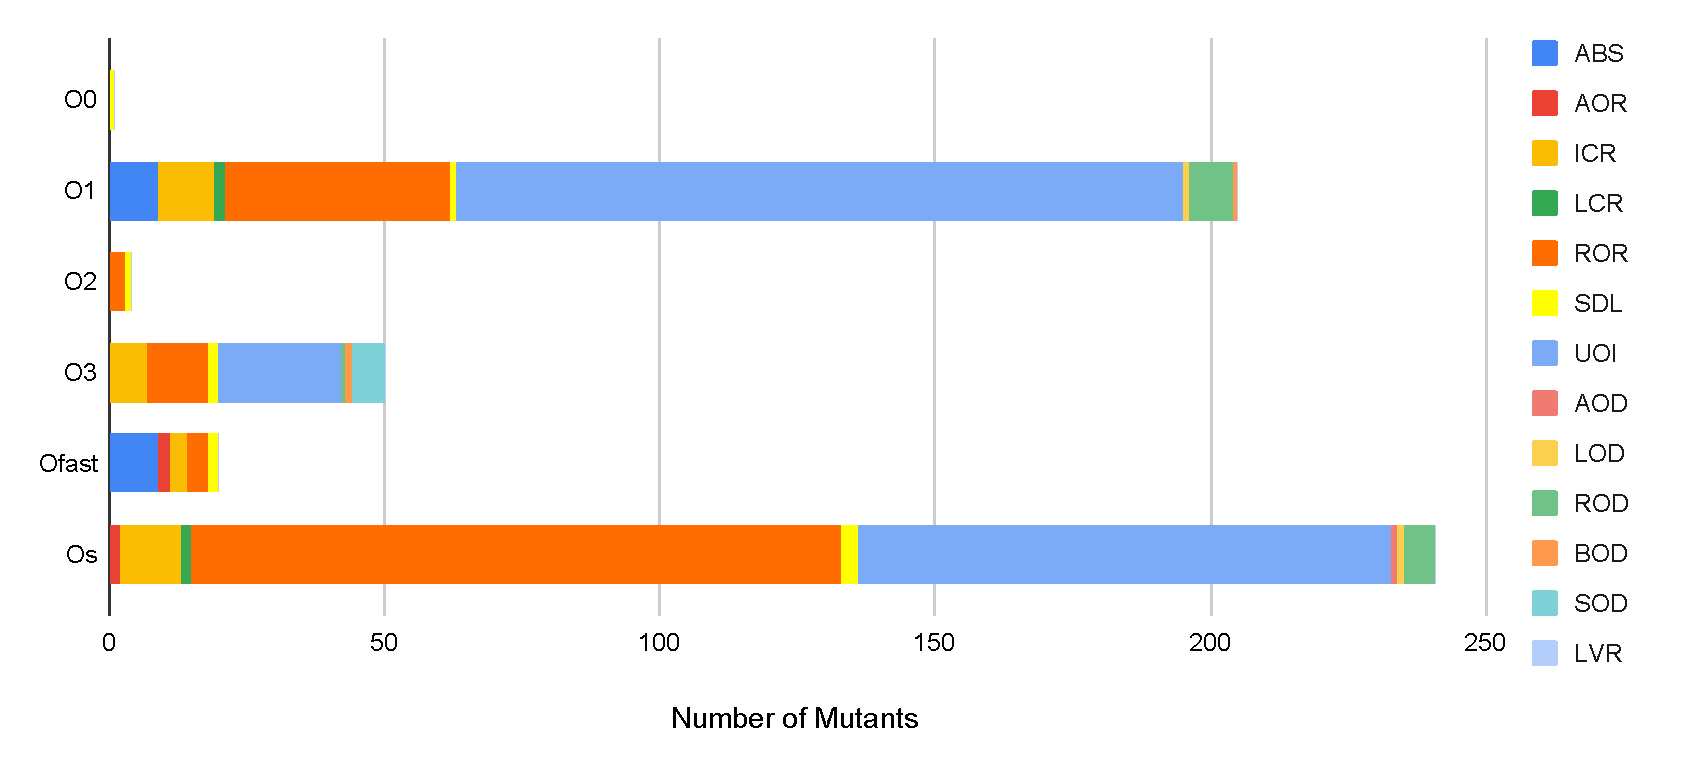
\includegraphics[width=9cm]{images/univ-eq}
\caption{Univocal, Trivially Equivalent Mutants detected by Compiler Optimizations.}
\label{fig:results:univeq}
\end{center}
\end{figure}

\begin{figure}[tb]
\begin{center}
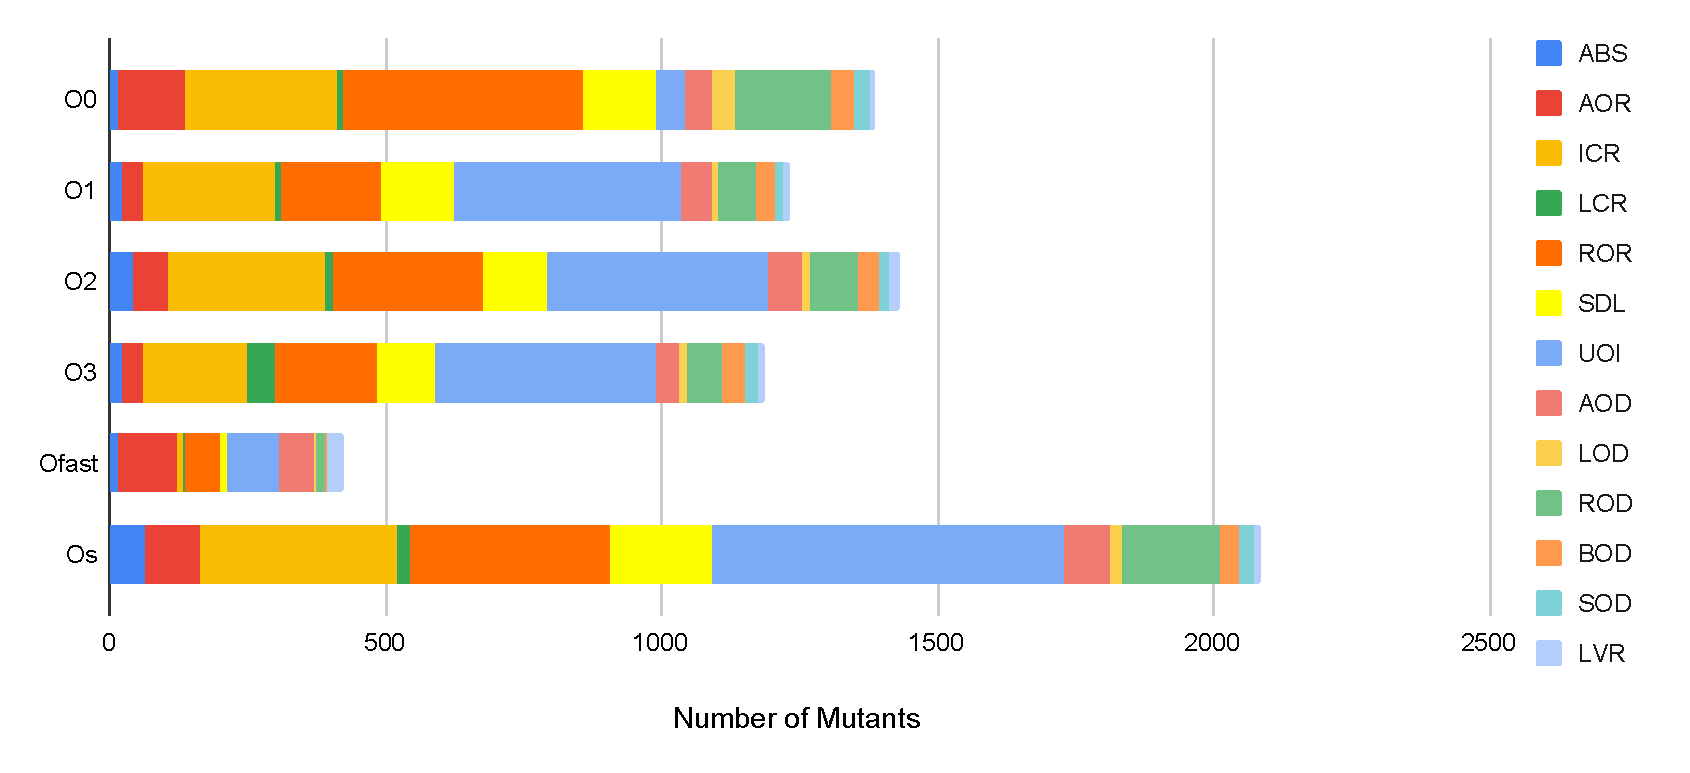
\includegraphics[width=9cm]{images/univ-red}
\caption{Univocal, Trivially Duplicate Mutants detected by Compiler Optimizations.}
\label{fig:results:univred}
\end{center}
\end{figure}




Table~\ref{table:results:compilerOptimizationsTime} provides the time required to compile the artifacts with the different optimization levels. Different from related work, which reports that optimization levels, in the worst case, lead an increase in compilation time by a factor of 5, \textbf{we do not observe a large difference in compilation time among the different optimization levels}. Indeed, in the worst case (i.e., option \emph{-Os}) this factor is $1.1$, an increase of 10\%. This directly results from the \APPR compilation pipeline, which minimizes the number of source files that need to be compiled. If developers can accept a compilation time increased by a factor of 5, as suggested in related work, all the compilation optimization levels can be applied, thus maximizing the number of equivalent and duplicate mutants being detected. In three out of five subjects, it takes less than a day to compile all the mutants with all the available optimization levels, which is acceptable, given the cost saved in subsequent steps. For the cases in which it may take multiple days, our practical solution consists in executing the compilation of the various mutants in parallel (e.g., on Cloud systems); for example, our toolset includes scripts to parallelize mutants compilation on HPC and cloud platforms. In the case of \SAIL{}\emph{-CSW}, the parallel compilation of 142,763 mutants, with the four available compilation options, can be performed in ~90 minutes using 100 nodes.



\subsection{RQ2 - Accuracy of Mutant Sampling Methods}
\label{sec:RQ2}
\paragraph{Design and measurements}


RQ2 aims to investigate  
%the validity of the findings reported by Zhang et al.~\cite{zhang2013operator} and, which concluded that 
to what extent the mutation score computed from a sample of mutants (hereafter, \INDEX{estimated mutation score}) accurately estimates the mutation score of the complete set of mutants (hereafter, \INDEX{actual mutation score}).

In our study, we consider the sampling strategies which are part of \APPR, as justified earlier: \INDEX{proportional uniform sampling}, \INDEX{proportional method-based sampling},  \INDEX{uniform fixed-size sampling}, and \INDEX{uniform FSCI sampling}. 


Because of the complexity and size of space software, combined with its high test execution cost, we are interested in selecting a very small subset of mutants. 
For this reason, 
to evaluate  \INDEX{proportional uniform sampling} and \INDEX{proportional method-based sampling},
we consider sampling ratios ranging from $1\%$ to $10\%$, in steps of $1\%$. Further,
 %to compare our results with those of Zhang et al., 
 we also cover the range 10\% to 100\%, in steps of $10\%$. To evaluate  \INDEX{uniform fixed-size sampling}, consistent with our earlier discussion, we consider a number of mutants in the range 100 to 1000, in steps of $100$.
Finally, to evaluate \INDEX{proportional method-based sampling}, we consider a threshold for the confidence interval (i.e., $T_{\mathit{CI}}$) that ranges from $0.05$ to $0.10$, in steps of $0.01$, with a confidence level of $95\%$, which is a common choice. The experiments conducted to address RQ2 entail the execution of the entire test suite for every sampled mutant. Executions with a prioritized and reduced test suite are addressed in Section~\ref{exp:accuracy:prioritize}. The evaluation of different values for $T_{\mathit{CI}}$ enable us to determine the costs associated with a more accurate estimation of the mutation score, in order to better understand the trade-offs.


We compute the actual mutation score of each system by executing the test suite against all the mutants that were successfully compiled, excluding mutants detected as being equivalent or duplicate by simple compiler optimization techniques (see RQ1). 
For each sampling ratio, to account for randomness,
we repeat the analysis 100 times, i.e., we compute the mutation score 100 times, based on 100 randomly selected subsets of mutants.
%we randomly select 100 subsets of mutants and compute their mutation score. 
Since it is not feasible to test all the mutants generated for \SAIL{}\emph{-CSW}, as discussed above, we focus on $\mathit{\SAIL{}}_{S}$.



%
%Computation in R: 
%X = set of 100 mutation scores
%quantile(X, c(.025, .975))

% s = standard deviation = sd(X)
% true_score = true mutation score
%z.test(X, sigma.x=s, mu=true_score)
%t.test(X, mu=true_score)
%
Our goal is to determine if the estimated mutation score is an accurate estimate of the actual mutation score.
This happens when the estimated mutation score differs from the actual mutation score for less than a small delta (hereafter, accuracy delta, $\delta_{acc}$) for a large percentage of the runs (e.g., 95\%).
We thus study the distribution of the difference between the estimated and actual mutation scores across all runs. More precisely, we estimate the 2.5\% and 97.5\% quantiles\footnote{We rely on linear interpolation using the type 8 
algorithm suggested in Hyndman and Fan~\cite{Hyndman1996}. It does not make assumptions about the underlying distribution.}.
Since these two quantiles delimit 95\% of the population,
we consider the mutation scores to be accurately estimated when they are within a pre-defined small range of the actual score [$-\delta_{acc}$;$+\delta_{acc}$].
In other words, we consider the estimated mutation score to be accurate when 
%the largest absolute value for the two quantiles is below $\delta_{acc}$.
the absolute value of the largest difference between quantiles and the actual score is below $\delta_{acc}$.
Since the range of acceptable mutation score values is small (75\%-100\%, see Section~1.2.1.1 from D2), we decided to use a threshold of 5\%, which is more conservative than that reported in related work ~\cite{gopinath2015hard}. 

Below, we analyze $\delta_{acc}$ for varying sampling rates. To improve readability, we discuss the results concerning the different sampling strategies separately.
% \emph{proportional uniform sampling} and \emph{proportional method-based sampling}.

% (i.e., the max difference between the actual mutation score and either the 2.5\% quantile or the 97.5\% quantile is below 0.01).

%%Since mutants are selected in random order and their result do not depend on the order in which they are executed, they can be treated as  independent from each other. 
%%We thus perform a t-test (alpha = 0.05) to test if the null hypothesis \emph{the mean mutation score of the sampled subset of mutants is equal to the true mutation score}, is rejected.


\paragraph{Results - proportional uniform sampling}

%\begin{figure}[tb]
%\begin{center}
%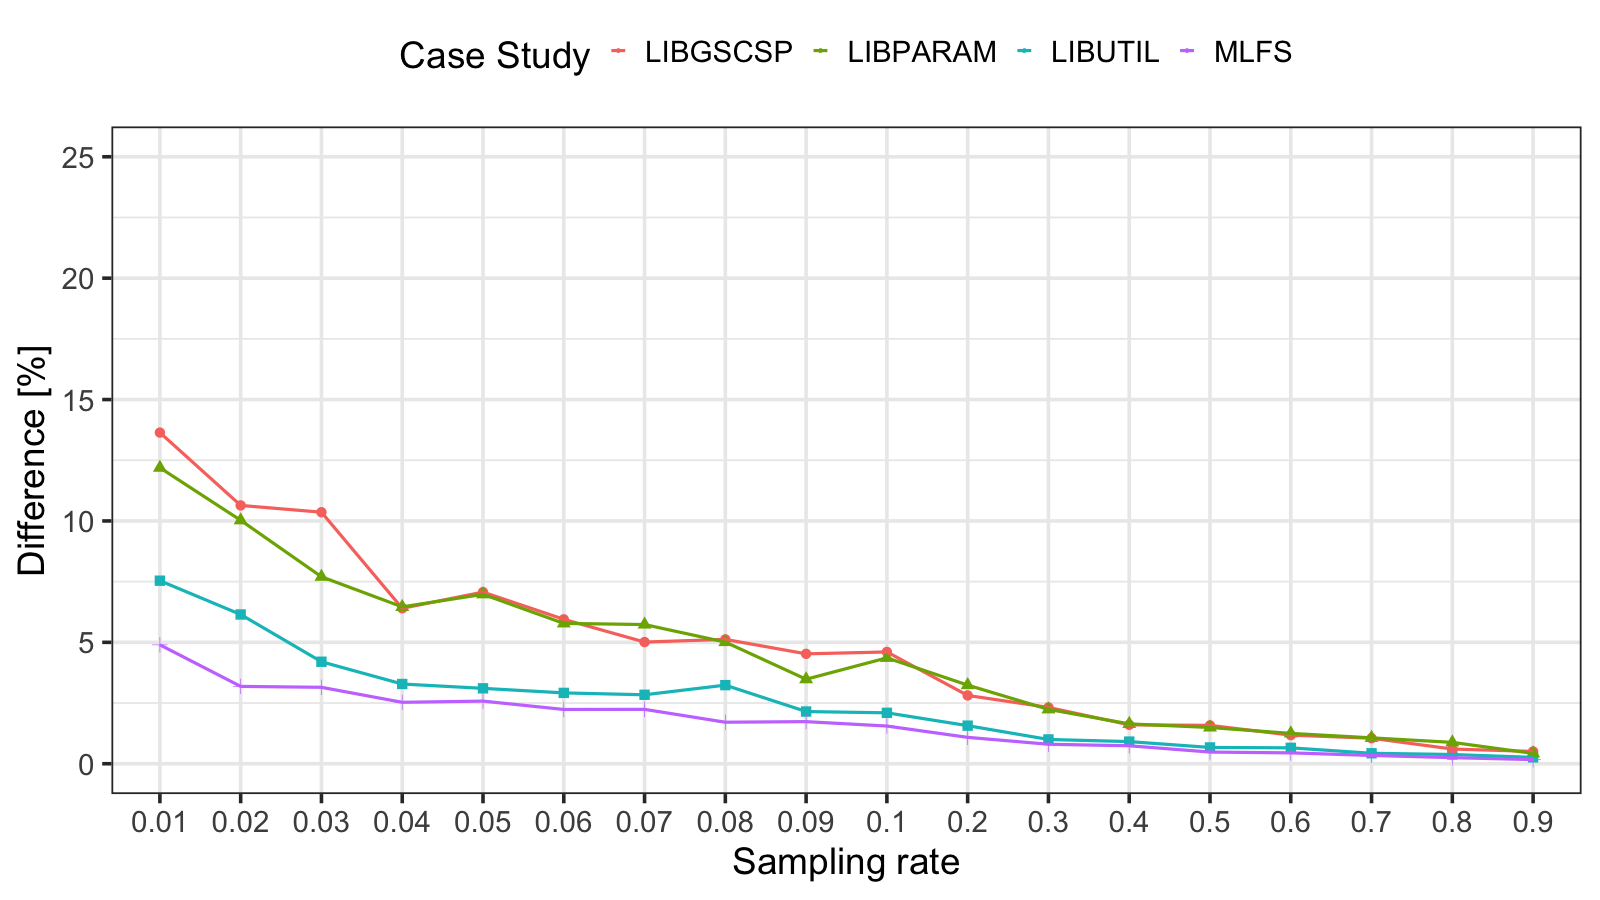
\includegraphics[width=9cm]{images/sampling_regular}
%\caption{Difference between estimated and actual mutation score (i.e., $\delta_{acc}$) for random sampling with different sampling rates.}
%\label{fig:approach}
%\end{center}
%\end{figure}
%
%\begin{figure}[tb]
%\begin{center}
%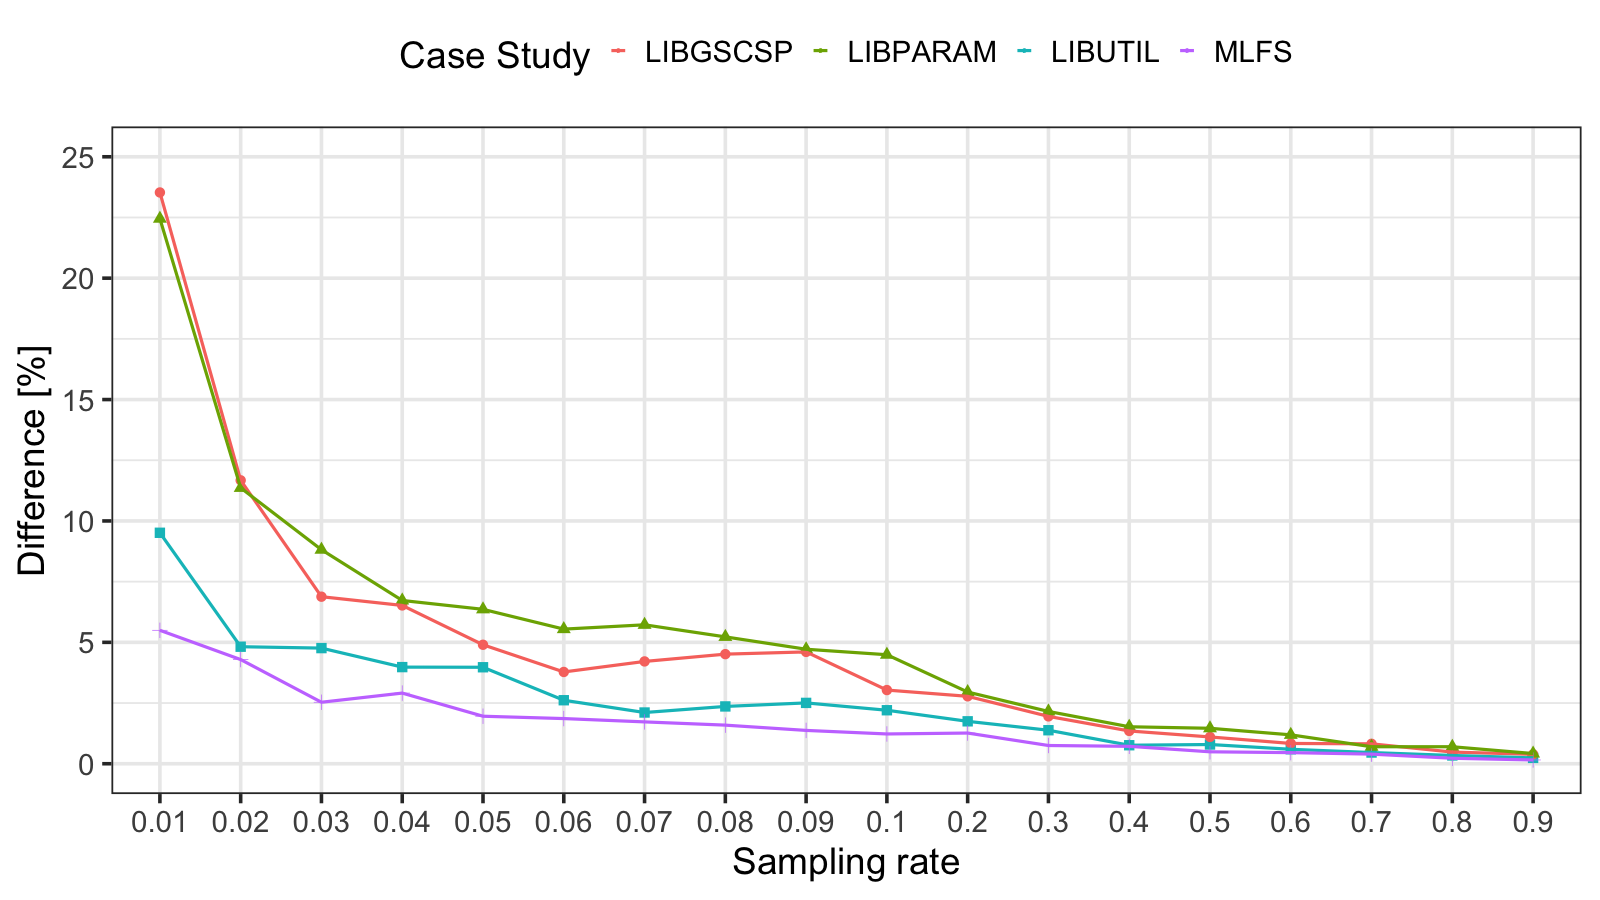
\includegraphics[width=9cm]{images/sampling_func}
%\caption{}
%\label{fig:results:sampling_func}
%\end{center}
%\end{figure}

% !TEX root =  ../Main.tex

\begin{table}[htb]
\caption{Actual mutation scores for artifacts.}
\label{table:results:accuracy:full} 
\scriptsize
\centering
\begin{tabular}{|
@{\hspace{1pt}}p{15mm}|
@{\hspace{1pt}}>{\raggedleft\arraybackslash}p{10mm}@{\hspace{1pt}}|
>{\raggedleft\arraybackslash}p{7mm}@{\hspace{1pt}}|
>{\raggedleft\arraybackslash}p{7mm}@{\hspace{1pt}}|
 >{\raggedleft\arraybackslash}p{25mm}@{\hspace{1pt}}|
}
\hline
\textbf{Case Study}&\textbf{Mutants}&\textbf{Killed}&\textbf{Live}&\textbf{Mutation Score (\%)}\\ 
\hline
$\mathit{ESAIL}_{S}$ &  &  &  &\\
$\mathit{LIBUTIL}$ &20261 & 13590 & 6671 & 71.20 \\
$\mathit{LIBPARAM}$&6435&4291&2144&69.12 \\
$\mathit{LIBGSCSP}$&7878&4905&2973&65.64 \\
$\mathit{MLFS}$&28069&22523&5546&81.80 \\
\hline
\end{tabular}

\end{table}
% !TEX root =  ../Main.tex

\begin{table}[htb]
\caption{RQ2. Accuracy of proportional uniform sampling.}
\label{table:results:accuracy:regSampling} 
\scriptsize
\centering
\begin{tabular}{|
@{\hspace{1pt}}p{5mm}|
@{\hspace{1pt}}>{\raggedleft\arraybackslash}p{7mm}@{\hspace{1pt}}|
>{\raggedleft\arraybackslash}p{5mm}@{\hspace{1pt}}|
>{\raggedleft\arraybackslash}p{6mm}@{\hspace{1pt}}|
 >{\raggedleft\arraybackslash}p{5mm}@{\hspace{1pt}}|
  >{\raggedleft\arraybackslash}p{6mm}@{\hspace{1pt}}|
@{\hspace{1pt}}>{\raggedleft\arraybackslash}p{5mm}@{\hspace{1pt}}|
@{\hspace{1pt}}>{\raggedleft\arraybackslash}p{7mm}@{\hspace{1pt}}|
>{\raggedleft\arraybackslash}p{5mm}@{\hspace{1pt}}|
 >{\raggedleft\arraybackslash}p{8mm}@{\hspace{1pt}}|
  >{\raggedleft\arraybackslash}p{5mm}@{\hspace{1pt}}|
}
\hline
     & \multicolumn{2}{c|}{\textbf{LIBGSCSP}} & \multicolumn{2}{c|}{\textbf{LIBPARAM}} & \multicolumn{2}{c|}{\textbf{LIBUTIL}} & \multicolumn{2}{c|}{\textbf{MLFS}} & \multicolumn{2}{c|}{\textbf{ESAIL}} \\
\hline
\textbf{r=} & \textbf{\#M}&\textbf{$\delta_{acc}$}& \textbf{\#M}&\textbf{$\delta_{acc}$}& \textbf{\#M}&\textbf{$\delta_{acc}$}& \textbf{\#M}&\textbf{$\delta_{acc}$}& \textbf{\#M}&\textbf{$\delta_{acc}$}               \\
\hline
0.01 & 50 & 13.64    			 & 40 & 12.19    			& 146 & 7.54    		& 214 & \textbf{4.90} &   36    & 14.04\\
0.02 & 100 & 10.64    			 & 79 & 10.03    			& 292 & 6.15    		& 428 & \textbf{3.19} &   71    & 11.84\\
0.03 & 150 & 10.36   			 & 118 & 7.70     			& 438 & \textbf{4.20}    & 642 & \textbf{3.15} &   107    & 8.84\\
0.04 & 200 & 6.40     			 & 158 & 6.46     			& 583 & \textbf{3.28}    & 855 & \textbf{2.53} &   142    & 7.92 \\
0.05 & 250 & 7.07     			 & 197 & 6.98     			& 729 & \textbf{3.11}    & 1069 & \textbf{2.58} &  177 & 6.39 \\
0.06 & 299 & 5.95    		 	 & 236 & 5.78     			& 875 & \textbf{2.92}    & 1283 & \textbf{2.24} & 213      &  6.25\\
0.07 & 349 & 5.01     			 & 276 & 5.73     		    & 1021 & \textbf{2.84}    & 1497 & \textbf{2.24} &  248     & 5.20 \\
0.08 & 399 & 5.12    		     & 315 & 5.01 		    	& 1166 & \textbf{3.24}    & 1710 & \textbf{1.71} &  283     & 5.68\\
0.09 & 449 & \textbf{4.53}     	 & 354 & \textbf{3.48}      & 1312 & \textbf{2.15}    & 1924 & \textbf{1.73} &  319     & \textbf{4.55}\\
0.10  & 499 & \textbf{4.61}      & 394 & \textbf{4.36}      & 1458 & \textbf{2.10}    & 2138 & \textbf{1.55} &  354     & \textbf{5.26}\\
0.20  & 997 & \textbf{2.81}      & 787 & \textbf{3.24}      & 2915 & \textbf{1.57}    & 4275 & \textbf{1.09} &    708   & \textbf{3.52}\\
0.30  & 1495 & \textbf{2.32}     & 1180 & \textbf{2.24}     & 4373 & \textbf{1.00}    & 6413 & \textbf{0.80} &  1061 & \textbf{2.56}\\
0.40  & 1993 & \textbf{1.60}     & 1573 & \textbf{1.64}     & 5830 & \textbf{0.91}    & 8550 & \textbf{0.74} &  1415 & \textbf{2.04}\\
0.50  & 2491 & \textbf{1.58}     & 1965 & \textbf{1.49}     & 7287 & \textbf{0.67}    & 10688 & \textbf{0.48} & 1768  & \textbf{1.50}\\
0.60  & 2990 & \textbf{1.18}     & 2358 & \textbf{1.25}     & 8745 & \textbf{0.66}    & 12825 & \textbf{0.45} & 2122  & \textbf{1.28}\\
0.70  & 3488 & \textbf{1.05}     & 2750 & \textbf{1.07}     & 10202 & \textbf{0.43}    & 14963 & \textbf{0.34} & 2476   & \textbf{1.16}\\
0.80  & 3986 & \textbf{0.61}     & 3143 & \textbf{0.88}     & 11660 & \textbf{0.38}    & 17100 & \textbf{0.25} & 2829   & \textbf{0.92}\\
0.90  & 4484 & \textbf{0.51}     & 3534 & \textbf{0.43}     & 13117 & \textbf{0.26}   & 19238 & \textbf{0.17} & 3183& \textbf{0.55}\\
\hline 
\end{tabular}

Note: \#M, number of mutants. Accurate results (i.e., $\delta_{acc} \le 5\%$) are in bold.
\end{table}

\begin{table}[htb]
\caption{RQ2. Accuracy of proportional method-based sampling.}
\label{table:results:accuracy:methodBased} 
\scriptsize
\centering
\begin{tabular}{|
@{\hspace{1pt}}p{5mm}|
@{\hspace{1pt}}>{\raggedleft\arraybackslash}p{7mm}@{\hspace{1pt}}|
>{\raggedleft\arraybackslash}p{5mm}@{\hspace{1pt}}|
>{\raggedleft\arraybackslash}p{6mm}@{\hspace{1pt}}|
 >{\raggedleft\arraybackslash}p{5mm}@{\hspace{1pt}}|
  >{\raggedleft\arraybackslash}p{6mm}@{\hspace{1pt}}|
@{\hspace{1pt}}>{\raggedleft\arraybackslash}p{5mm}@{\hspace{1pt}}|
@{\hspace{1pt}}>{\raggedleft\arraybackslash}p{7mm}@{\hspace{1pt}}|
>{\raggedleft\arraybackslash}p{5mm}@{\hspace{1pt}}|
 >{\raggedleft\arraybackslash}p{8mm}@{\hspace{1pt}}|
  >{\raggedleft\arraybackslash}p{5mm}@{\hspace{1pt}}|
}
\hline
     & \multicolumn{2}{c|}{\textbf{LIBGSCSP}} & \multicolumn{2}{c|}{\textbf{LIBPARAM}} & \multicolumn{2}{c|}{\textbf{LIBUTIL}} & \multicolumn{2}{c|}{\textbf{MLFS}} & \multicolumn{2}{c|}{\textbf{ESAIL}} \\
\hline
\textbf{r=} & \textbf{\#M}&\textbf{$\delta_{acc}$}& \textbf{\#M}&\textbf{$\delta_{acc}$}& \textbf{\#M}&\textbf{$\delta_{acc}$}& \textbf{\#M}&\textbf{$\delta_{acc}$}& \textbf{\#M}&\textbf{$\delta_{acc}$}               \\
\hline
0.01 & 19 & 23.53    			 & 15 & 22.45    			& 111 & 9.51    		 & 232 & 5.50 &  33& 13.84\\
0.02 & 75 & 11.67    			 & 77 & 11.36    			& 250 & \textbf{4.82}    & 447 & \textbf{4.29} &64& 16.18\\
0.03 & 131 & 6.88    			 & 120 & 8.82    			 & 422 & \textbf{4.76}   & 661 & \textbf{2.53} &104   &8.63\\
0.04 & 194 & 6.52    			 & 165 & 6.73    			 & 564 & \textbf{3.98}   & 881 & \textbf{2.91} &137 &9.93\\
0.05 & 258 & \textbf{4.90}     & 208 & 6.36     			& 731 & \textbf{3.97}    & 1094 & \textbf{1.96} &178   &6.84\\
0.06 & 312 & \textbf{3.78}     & 254 & 5.54     			& 905 & \textbf{2.62}    & 1306 & \textbf{1.86} &223& 6.18\\
0.07 & 368 & \textbf{4.21}     & 290 & 5.72     			& 1045 & \textbf{2.11}    & 1517 & \textbf{1.72} &254& 5.72\\
0.08 & 417 & \textbf{4.51}     & 335 & 5.22     			& 1197 & \textbf{2.36}    & 1733 & \textbf{1.59} & 287&\textbf{4.67}\\
0.09 & 466 & \textbf{4.61}     & 378 & \textbf{4.72}    	 & 1353 & \textbf{2.51}    & 1942 & \textbf{1.37} & 331      &\textbf{4.59}\\
0.1  & 515 & \textbf{3.03}     & 413 & \textbf{4.49}     	& 1512 & \textbf{2.20}    & 2159 & \textbf{1.23} &364&\textbf{3.87}\\
0.2  & 1030 & \textbf{2.78}     & 811 & \textbf{2.95}     	& 2963 & \textbf{1.75}    & 4295 & \textbf{1.26} & 721  & \textbf{2.95}\\
0.3  & 1523 & \textbf{1.95}     & 1210 & \textbf{2.15}     & 4446 & \textbf{1.38}    & 6430 & \textbf{0.75} & 1079&\textbf{2.76}\\
0.4  & 2045 & \textbf{1.35}     & 1605 & \textbf{1.52}     & 5942 & \textbf{0.76}    & 8576 & \textbf{0.72} & 1432&\textbf{1.81}\\
0.5  & 2518 & \textbf{1.10}     & 1985 & \textbf{1.46}     & 7361 & \textbf{0.79}    & 10702 & \textbf{0.49} & 1779&\textbf{1.42}\\
0.6  & 3035 & \textbf{0.84}     & 2395 & \textbf{1.19}     & 8853 & \textbf{0.60}    & 12863 & \textbf{0.46} & 2139&\textbf{1.22}\\
0.7  & 3550 & \textbf{0.82}     & 2791 & \textbf{0.70}     & 10334 & \textbf{0.46}    & 15007 & \textbf{0.40} & 2494&\textbf{1.03}\\
0.8  & 4027 & \textbf{0.48}     & 3178 & \textbf{0.70}     & 11779 & \textbf{0.34}    & 17134 & \textbf{0.23} & 2849&\textbf{0.86}\\
0.9  & 4527 & \textbf{0.39}     & 3574 & \textbf{0.42}     & 13228 & \textbf{0.24}    & 19272 & \textbf{0.16} & 3202&\textbf{0.62}\\
\hline
\end{tabular}

Note: \#M, number of mutants. Accurate results (i.e., $\delta_{acc} \le 5\%$) are in bold.
\end{table}




Table~\ref{table:results:accuracy:full} reports on the mutation scores obtained with the entire test suite for all subjects. 
As expected, the best mutation score is obtained for \MLFS{}{}, whose test suite achieves MC/DC coverage. \REVNOV{PTCR-20}{In this project, based on related work, we assume a good quality test suite to have a mutation score above 75\%. However, the objective of this report is not to evaluate the quality of the provided test suites based on the observed mutation score but to evaluate the approach for estimating the mutation score. A discussion of of the quality of the provided test suites based on the mutation score is an activity that might be left for later stages when the mutation testing approach is completed and partners had time to inspect live mutants. Indeed,
 there are a number of factors that affect the computed mutation score; for example, the presence of equivalent mutants lead to live mutants and, consequently, make the mutation score (erroneously) low. The inspection of equivalent mutants for the case studies is till ongoing, at this stage. Also, the reasons for not achieving a high mutation score may vary from case study to case study and needs an in depth investigation. For example, for GSL case studies, this seems to be related to a number of off-the-shelf components integrated in the source of the system. Such off-the-shelf-components are not expected to be tested by the test suite. A mutation score based on only non off-the-shelf-components will be computed in later stages of the project.}

%Figure~\ref{fig:results:accuracy:sampling}  reports a plot with the maximum absolute value of the difference...
Table~\ref{table:results:accuracy:regSampling} provides accuracy results (column $\delta_{acc}$) for proportional uniform sampling for a range of sampling rates~($r$). 
To enable comparisons across sampling methods, Column \emph{\#M} reports the number of mutants sampled for each sampling rate.
As expected, a larger sampling rate leads to more accurate results (i.e., low $\delta_{acc}$). 
We notice that for test suites that ensure MC/DC coverage (i.e., \MLFS{}{}), even a very small sampling ratio (i.e., 0.01) guarantees a $\delta_{acc}$ below 5\%. However, to achieve an accurate mutation score estimate across all subjects, a minimum sampling rate of 0.09 is required.

%Table~\ref{table:results:accuracy:sampling} reports, for every case study system, sampling strategy, and sampling ratio, the max difference between the actual mutation score and either the 2.5\%/97.5\% quantile.

%\FIXME{... We cannot go much below 5\%, but in certain systems 5\% is still a lot.}

In addition, we observe that, for $r=0.09$, the worst results (highest deltas) are observed for smaller projects, which indicates that \textbf{the estimation accuracy may not depend on the percentage of sampled mutants but on the size of the sample}; indeed, for most of the subjects, accurate results \CHANGED{(i.e., $\delta_{acc} < 5\%$)} are obtained with a number of mutants between 350 and 450. This aspect is further studied when considering  \INDEX{uniform fixed-size sampling} and \INDEX{uniform FSCI sampling}.

\paragraph{Results - proportional method-based sampling}

Table~\ref{table:results:accuracy:methodBased} shows the accuracy results for proportional method-based sampling. 
Interestingly, for two subjects (i.e., \GCSP{} and \UTIL{}), proportional method-based sampling leads to accurate estimates of the mutation score with a lower number of mutants than proportional uniform sampling (i.e., around 250).
However, to achieve accurate results with all subjects, we need a minimal sampling rate of $r=0.09$, as for proportional uniform sampling, which, in the case of method-based sampling, leads to a slightly higher number of mutants. For this reason, we do not see any benefit in using method-based sampling.




\paragraph{Results - uniform fixed-size sampling, uniform FSCI sampling}

%\begin{figure}[tb]
%\begin{center}
%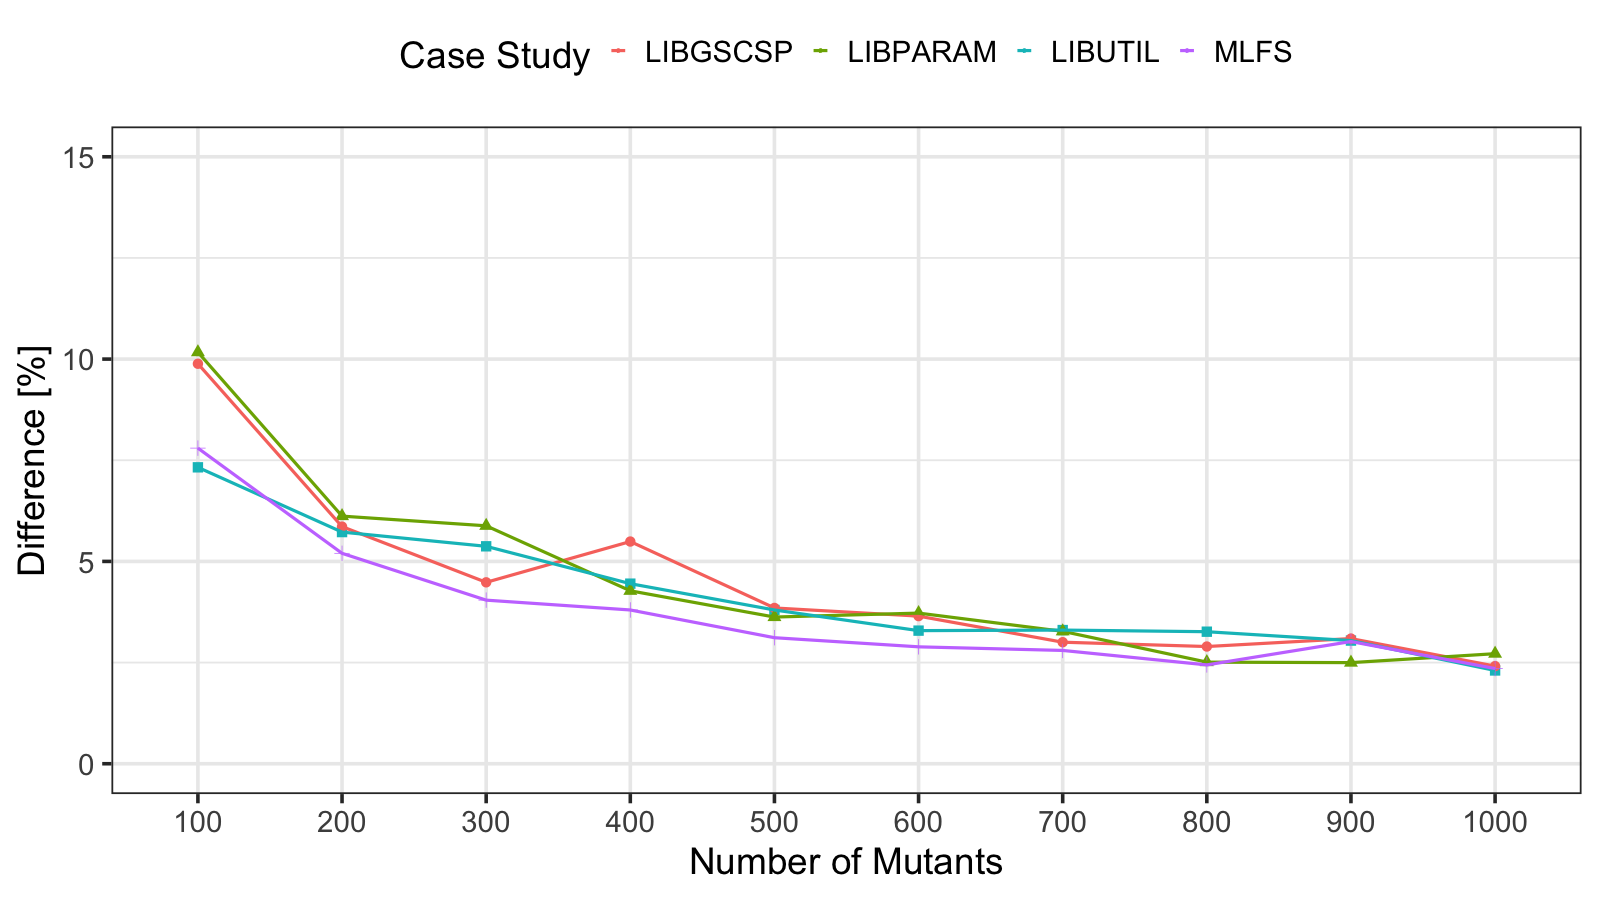
\includegraphics[width=6cm]{images/sampling_fixed}
%\caption{}
%\label{fig:results:fixedNumberOfMutants}
%\end{center}
%\end{figure}
% !TEX root =  ../Main.tex

\begin{table*}[htb]
\caption{RQ2. Accuracy with uniform fixed-size sampling and uniform FSCI sampling. }
\label{table:results:accuracy:FSCI:sampling} 
\scriptsize
\centering
\begin{tabular}{|
>{\raggedleft\arraybackslash}p{10mm}@{\hspace{1pt}}|
>{\raggedleft\arraybackslash}p{5mm}@{\hspace{1pt}}|
p{12mm}@{\hspace{1pt}}|
>{\raggedleft\arraybackslash}p{10mm}@{\hspace{1pt}}|
>{\raggedleft\arraybackslash}p{5mm}@{\hspace{1pt}}|
p{12mm}@{\hspace{1pt}}|
>{\raggedleft\arraybackslash}p{10mm}@{\hspace{1pt}}|
>{\raggedleft\arraybackslash}p{5mm}@{\hspace{1pt}}|
p{12mm}@{\hspace{1pt}}|
>{\raggedleft\arraybackslash}p{10mm}@{\hspace{1pt}}|
>{\raggedleft\arraybackslash}p{5mm}@{\hspace{1pt}}|
p{12mm}@{\hspace{1pt}}|
>{\raggedleft\arraybackslash}p{10mm}@{\hspace{1pt}}|
>{\raggedleft\arraybackslash}p{5mm}@{\hspace{1pt}}|
p{12mm}@{\hspace{1pt}}|
}
\hline
\multicolumn{3}{|c|}{\textbf{LIBGSCSP}}      & \multicolumn{3}{c|}{\textbf{LIBPARAM}}      & \multicolumn{3}{c|}{\textbf{LIBUTIL}}       & \multicolumn{3}{c|}{\textbf{MLFS}}          & \multicolumn{3}{c|}{\textbf{ESAIL}}       \\
\hline
\textbf{\#Mutants} & $\delta_{acc}$ & \textbf{Method}   & \textbf{\#Mutants} & $\delta_{acc}$ & \textbf{Method}   & \textbf{\#Mutants} & $\delta_{acc}$ & \textbf{Method}   & \textbf{\#Mutants} & $\delta_{acc}$ & \textbf{Method}   & \textbf{\#Mutants} & $\delta_{acc}$ & \textbf{Method} \\
\hline
100       & 9.88       & FIXED    & 100       & 10.17      & FIXED    & 100       & 7.32       & FIXED    & 100       & 7.80       & FIXED    &  100         &     8.89       &   FIXED     \\
200       & 5.86       & FIXED    & 200       & 6.12       & FIXED    & 200       & 5.73       & FIXED    & 200       & 5.20       & FIXED    &   200        &      6.14      &   FIXED     \\
300       & \textbf{4.48}       & FIXED    & 300       & 5.88       & FIXED    & 300       & 5.37       & FIXED    & 248       & \textbf{4.56}       & CI 0.1  &    300       &      5.53      &    FIXED    \\
364       & \textbf{4.42}       & FSCI 0.1  & 346       & \textbf{4.26}       & FSCI 0.1  & 333       & \textbf{4.73}       & FSCI 0.1  & 300       & \textbf{4.04}       & FIXED    &   366        &     \textbf{3.92}       &    FSCI 0.1    \\
400       & \textbf{5.49}       & FIXED    & 400       & \textbf{4.27}       & FIXED    & 400       & \textbf{4.45}       & FIXED    & 302       & \textbf{4.64}       & FSCI 0.09 &     400      &     \textbf{4.52}       &    FIXED    \\
447       & \textbf{3.70}       & FSCI 0.09 & 425       & \textbf{3.79}       & FSCI 0.09 & 409       & \textbf{4.08}       & FSCI 0.09 & 379       & \textbf{4.01}       & FSCI 0.08 &   449        &    \textbf{3.66}     &   FSCI 0.09    \\
500       & \textbf{3.85}       & FIXED    & 500       & \textbf{3.63}       & FIXED    & 500       & \textbf{3.80}       & FIXED    & 400       & \textbf{3.80}       & FIXED    &   500      &      \textbf{4.08}      &   FIXED     \\
564       & \textbf{3.53}       & FSCI 0.08 & 536       & \textbf{3.75}       & FSCI 0.08 & 514       & \textbf{3.94}       & FSCI 0.08 & 490       & \textbf{3.90}       & FSCI 0.07 &    567       &  \textbf{3.03}   &  FSCI 0.08      \\
600       & \textbf{3.65}       & FIXED    & 600       & \textbf{3.72}       & FIXED    & 600       & \textbf{3.29}       & FIXED    & 500       & \textbf{3.11}       & FIXED    &     600      &  \textbf{3.73}          &     FIXED   \\
700       & \textbf{3.00}       & FIXED    & 696       & \textbf{2.89}       & FSCI 0.07 & 668       & \textbf{3.99}       & FSCI 0.07 & 600       & \textbf{2.89}       & FIXED    &     700      &      \textbf{3.01}      &    FIXED    \\
734       & \textbf{3.62}       & FSCI 0.07 & 700       & \textbf{3.27}       & FIXED    & 700       & \textbf{3.30}       & FIXED    & 667       & \textbf{2.78}       & FSCI 0.06 &     738      &      \textbf{2.77}      &    FSCI 0.07    \\
800       & \textbf{2.90}       & FIXED    & 800       & \textbf{2.51}       & FIXED    & 800       & \textbf{3.26}       & FIXED    & 700       & \textbf{2.80}       & FIXED    &     800      &  \textbf{2.55}          &    FIXED    \\
900       & \textbf{3.09}       & FIXED    & 900       & \textbf{2.50}       & FIXED    & 900       & \textbf{3.04}       & FIXED    & 800       & \textbf{2.44}       & FIXED    &     900      &  \textbf{2.37}          &    FIXED    \\
994       & \textbf{3.00}       & FSCI 0.06 & 945       & \textbf{2.42}       & FSCI 0.06 & 906       & \textbf{3.28}       & FSCI 0.06 & 900       & \textbf{3.02}       & FIXED    &  998         &  \textbf{2.65}         &   FSCI 0.06     \\
1000      & \textbf{2.41}       & FIXED    & 1000      & \textbf{2.72}       & FIXED    & 1000      & \textbf{2.31}       & FIXED    & 960       & \textbf{2.31}       & FSCI 0.05 & 1000     &  \textbf{2.96}          &   FIXED     \\
1422      & \textbf{2.44}       & FSCI 0.05 & 1352      & \textbf{1.93}       & FSCI 0.05 & 1298      & \textbf{2.72}       & FSCI 0.05 & 1000      & \textbf{2.35}       & FIXED    &    1429     &    \textbf{1.70}        &  FSCI 0.05 \\
\hline
\end{tabular}

Accurate results (i.e., $\delta_{acc} \le 5\%$) are in bold.
\end{table*}

Table~\ref{table:results:accuracy:FSCI:sampling} shows the accuracy results for uniform fixed-size sampling and uniform FSCI sampling. For each subject, we sort results according to the number of mutants. For FSCI sampling, we report the confidence interval threshold $T_\mathit{CI}$. 

The best results (i.e., lowest number of mutants with $\delta_{acc} \le 5\%$) are obtained using  FSCI sampling with $T_\mathit{CI}=0.10$. Predictably, FSCI sampling with $T_\mathit{CI}=0.10$ guarantees $\delta_{acc} \le 5\%$ (half of $T_\mathit{CI}$); indeed, by construction, if our assumptions 
on the limited correlation between mutants and the mutation score following a  binomial distribution hold (see Section~1.2.1.4 from D2),
FSCI sampling with $T_\mathit{CI}=0.10$ is expected to guarantee $\delta_{acc} \le 5\%$ (see Appendix
B
%~\ref{appendix:correlation} 
for further details on the distribution of the mutation score across subjects).

In addition, our results suggest that a limited number of mutants (between 300 and 400) is required to achieve the desired $\delta_{acc}$. This sample size is much lower than the (worst case) sample size proposed by Gopinath et al., which is 1,000~\cite{gopinath2015hard}. Also, our sample size is smaller 
than the one estimated, for a mutation score between 60\% and 80\%, by 
approaches
%a priori approaches 
based on confidence-interval estimation, which is still around 1,000~\cite{Goncalves2012}. 
%that could be estimated a priori for a mutation score between 60\% and 80\%, which is around 1,000~\cite{Goncalves2012}. 
However, we confirm the finding of Gopinath et al., who demonstrated that the binomial distribution %provides a conservative estimation of the
accurately estimates the mutation score~\cite{gopinath2015hard}.

To summarize, this is the first study demonstrating that \textbf{FSCI sampling is the 
best approach for obtaining the smallest sample size
%optimal approach for determining sample size 
while providing guarantees on the accuracy of mutation score estimates.} 
We therefore propose a better solution than that of Gopinath et al., who provide an upper bound for the number of mutants to be considered in uniform fixed-size sampling, since we have evidence suggesting that FSCI sampling helps to select a significantly smaller sample size for a desired confidence interval.





\subsection{RQ3 - SDL accuracy}



\paragraph{Design and measurements}


RQ3 assesses if mutants generated using only deletion operators can accurately estimate the mutation score of the complete mutants set.

To this end, we study the difference between the mutation score obtained by executing the entire test suite on the mutants generated with all the operators (i.e., the actual mutation score) and the mutation score obtained with either (1) the mutants generated with the SDL operator only, or (2) the mutants generated with both the SDL and OODL operators.
As for RQ2, to be accurate, the mutation score obtained with a subset of operators should differ by at most 5\%.


\paragraph{Results}

% !TEX root =  ../Main.tex

\begin{table}[htb]
\caption{Comparison of mutation scores obtained with mutants generated using all operators, the SDL operator only, and the SDL + OODL operators.}
\label{table:results:score:sdl:oodl} 
\scriptsize
\centering
\begin{tabular}{|
@{\hspace{1pt}}p{15mm}|
 >{\raggedleft\arraybackslash}p{8mm}@{\hspace{1pt}}|
  >{\raggedleft\arraybackslash}p{13mm}@{\hspace{1pt}}|
 >{\raggedleft\arraybackslash}p{6mm}@{\hspace{1pt}}|
  >{\raggedleft\arraybackslash}p{15mm}@{\hspace{1pt}}|
   >{\raggedleft\arraybackslash}p{15mm}@{\hspace{1pt}}|
}
\hline
\textbf{Case Study}&\multicolumn{2}{c|}{\textbf{\# Mutants}}&\multicolumn{3}{c|}{\textbf{Mutation score}}\\ 
&SDL&SDL+OODL&ALL&SDL&SDL+OODL\\
\hline
$\mathit{ESAIL}_{S}$ &	701&	974& 65.36 & 61.91 (-3.45) & 63.45 (-1.91) \\
$\mathit{LIBGSCSP}$ & 912	&1546	&65.64 &70.72 (+5.08) &71.35 (+5.71)\\
$\mathit{LIBPARAM}$ & 731&1324	&69.12 &64.84 (-4.28) &66.39 (+2.73)\\
$\mathit{LIBUTIL}$ 	 &2341	&3811	&71.20 & 73.26 (+2.06) &72.63 (+1.43)\\
$\mathit{MLFS}$ &1729	&	5971	&81.80 &85.71 (3.91)& 88.03 (+6.23)\\
\hline
\end{tabular}

\end{table}

In Table~\ref{table:results:score:sdl:oodl}, column \emph{\# Mutants} shows, for each subject, the number of mutants generated with either the SDL operator or both the SDL and OODL operators. 
Column \emph{Mutation score} shows the mutation score obtained when using the entire test suite to exercise the mutants generated with either all the operators, the SDL operator only, or both the SDL and OODL operators. Between parentheses, we also report the difference between the mutation score obtained with all the operators and that obtained with a subset of operators. Results show that, for some of our subjects, the mutation score obtained with the SDL operator does not accurately estimate the mutation score obtained with a broader set of operators. Though these results do not invalidate related work~\cite{delamaro2014experimental}, whose focus is on the evaluation of the strength of SDL and OODL operators, it shows that \textbf{SDL and OODL operators should not be adopted to estimate the mutation score computed with a larger set of operators}. We leave the evaluation of the strength of SDL and OODL operators to future work.




%is always accurate; instead, the mutation score obtained with both the SDL and OODL operators is not accurate in the case of MLFS.}

%Tables~\ref{table:results:accuracy:regSamplingSDL} to~\ref{table:results:accuracy:funcSamplingSDLOODL} show the accuracy of proportional uniform and method-based sampling applied to select mutants generated either with the SDL operator only or with the SDL and OODL operators. 
%Tables~\ref{table:results:accuracy:sampling_sdl} and~\ref{table:results:accuracy:sampling_sdl_oodl} show the accuracy of uniform fixed-size sampling and uniform FSCI sampling applied to select mutants generated either with the SDL operator only or with both the SDL and OODL operators. In all the cases, it is not possible to identify any sampling rate that enable an accurate  (i.e., $\delta_{acc} \le 5\%$) estimation of the mutation score. \FIXME{This is mostly due which might be partially due to the overall number of mutants being generated being low.}
%
%
%\FIXME{We suggest to rely on SDL/SLD+OODL...}

%% !TEX root =  ../Main.tex
\begin{table}[htb]
\caption{RQ3. 
Accuracy of proportional uniform sampling applied to select SDL mutants only.}
\label{table:results:accuracy:regSamplingSDL} 
\scriptsize
\centering
\begin{tabular}{|
@{\hspace{1pt}}p{5mm}|
@{\hspace{1pt}}>{\raggedleft\arraybackslash}p{7mm}@{\hspace{1pt}}|
>{\raggedleft\arraybackslash}p{5mm}@{\hspace{1pt}}|
>{\raggedleft\arraybackslash}p{6mm}@{\hspace{1pt}}|
 >{\raggedleft\arraybackslash}p{5mm}@{\hspace{1pt}}|
  >{\raggedleft\arraybackslash}p{6mm}@{\hspace{1pt}}|
@{\hspace{1pt}}>{\raggedleft\arraybackslash}p{5mm}@{\hspace{1pt}}|
@{\hspace{1pt}}>{\raggedleft\arraybackslash}p{7mm}@{\hspace{1pt}}|
>{\raggedleft\arraybackslash}p{5mm}@{\hspace{1pt}}|
 >{\raggedleft\arraybackslash}p{8mm}@{\hspace{1pt}}|
  >{\raggedleft\arraybackslash}p{5mm}@{\hspace{1pt}}|
}
\hline
     & \multicolumn{2}{c|}{\textbf{LIBGSCSP}} & \multicolumn{2}{c|}{\textbf{LIBPARAM}} & \multicolumn{2}{c|}{\textbf{LIBUTIL}} & \multicolumn{2}{c|}{\textbf{MLFS}} & \multicolumn{2}{c|}{\textbf{ESAIL}} \\
\hline
\textbf{r=} & \textbf{\#M}&\textbf{$\delta_{acc}$}& \textbf{\#M}&\textbf{$\delta_{acc}$}& \textbf{\#M}&\textbf{$\delta_{acc}$}& \textbf{\#M}&\textbf{$\delta_{acc}$}& \textbf{\#M}&\textbf{$\delta_{acc}$}               \\
\hline           
0.01 & 10 & 34.36    & 8 & 38.18     & 24 & 16.30   & 18 & 20.69 &       \\
0.02 & 19 & 23.83    & 15 & 29.12    & 47 & 13.91   & 35 & 15.34 &       \\
0.03 & 28 & 20.07    & 22 & 23.67    & 71 & 14.72   & 52 & 12.43 &       \\
0.04 & 37 & 19.56    & 30 & 20.87    & 94 & 11.27   & 70 & 11.06 &       \\
0.05 & 46 & 18.11    & 37 & 17.77    & 118 & 9.31    & 87 & 10.15 &       \\
0.06 & 55 & 15.32    & 44 & 21.39    & 141 & 9.31    & 104 & 9.09  &       \\
0.07 & 64 & 15.61    & 52 & 16.28    & 164 & 9.64    & 122 & 9.18  &       \\
0.08 & 73 & 13.81    & 59 & 16.58    & 188 & 6.99    & 139 & 9.57  &       \\
0.09 & 83 & 11.53    & 66 & 16.16    & 211 & 8.20    & 156 & 8.28  &       \\
0.1  & 92 & 13.19    & 74 & 15.07    & 235 & 7.97    & 173 & 9.25  &       \\
0.2  & 183 & 10.32    & 147 & 9.94     & 469 & 5.25    & 346 & 6.64  &       \\
0.3  & 274 & 9.91     & 220 & 9.12     & 703 & \textbf{4.91}    & 519 & 7.13  &       \\
0.4  & 365 & 8.48     & 292 & 8.73     & 937 & \textbf{4.43}    & 692 & 6.06  &       \\
0.5  & 456 & 8.07     & 364 & 7.38     & 1171 & \textbf{3.61}    & 865 & 5.60  &       \\
0.6  & 548 & 7.17     & 438 & 7.28     & 1405 & \textbf{3.50}    & 1038 & 5.25  &       \\
0.7  & 639 & 6.90     & 510 & 5.86     & 1639 & \textbf{3.27}    & 1211 & \textbf{4.91}  &       \\
0.8  & 730 & 6.56     & 582 & 5.79     & 1873 & \textbf{2.80}    & 1384 & \textbf{4.87}  &       \\
0.9  & 821 & 5.86     & 655 & 5.22     & 2107 & \textbf{2.58}    & 1557 & \textbf{4.49}  &   \\
\hline   
\end{tabular}
Note: \#M, number of mutants. Accurate results (i.e., $\delta_{acc} \le 5\%$) are in bold.
\end{table}


\begin{table}[htb]
\caption{RQ3. 
Accuracy of proportional method-based sampling applied to select SDL mutants only.}
\label{table:results:accuracy:funcSamplingSDL} 
\scriptsize
\centering
\begin{tabular}{|
@{\hspace{1pt}}p{5mm}|
@{\hspace{1pt}}>{\raggedleft\arraybackslash}p{7mm}@{\hspace{1pt}}|
>{\raggedleft\arraybackslash}p{5mm}@{\hspace{1pt}}|
>{\raggedleft\arraybackslash}p{6mm}@{\hspace{1pt}}|
 >{\raggedleft\arraybackslash}p{5mm}@{\hspace{1pt}}|
  >{\raggedleft\arraybackslash}p{6mm}@{\hspace{1pt}}|
@{\hspace{1pt}}>{\raggedleft\arraybackslash}p{5mm}@{\hspace{1pt}}|
@{\hspace{1pt}}>{\raggedleft\arraybackslash}p{7mm}@{\hspace{1pt}}|
>{\raggedleft\arraybackslash}p{5mm}@{\hspace{1pt}}|
 >{\raggedleft\arraybackslash}p{8mm}@{\hspace{1pt}}|
  >{\raggedleft\arraybackslash}p{5mm}@{\hspace{1pt}}|
}
\hline
     & \multicolumn{2}{c|}{\textbf{LIBGSCSP}} & \multicolumn{2}{c|}{\textbf{LIBPARAM}} & \multicolumn{2}{c|}{\textbf{LIBUTIL}} & \multicolumn{2}{c|}{\textbf{MLFS}} & \multicolumn{2}{c|}{\textbf{ESAIL}} \\
\hline
\textbf{r=} & \textbf{\#M}&\textbf{$\delta_{acc}$}& \textbf{\#M}&\textbf{$\delta_{acc}$}& \textbf{\#M}&\textbf{$\delta_{acc}$}& \textbf{\#M}&\textbf{$\delta_{acc}$}& \textbf{\#M}&\textbf{$\delta_{acc}$}               \\
\hline
0.01 & NA       			& NA       		& 4 & 28.80   			& 4 & 31.80 &       \\
0.02 & NA       			& 2 & 69.12    & 15 & 28.80   			& 20 & 18.20 &       \\
0.03 & 2 & 34.36    		& 8 & 44.12    & 28 & 18.09   			& 35 & 15.34 &       \\
0.04 & 10 & 34.36    		& 9 & 35.79    & 44 & 15.16   			& 76 & 12.94 &       \\
0.05 & 12 & 26.03    		& 9 & 35.79    & 64 & 14.00   			& 88 & 11.98 &       \\
0.06 & 15 & 21.03    		& 19 & 24.51    & 88 & 10.62  			 & 109 & 9.94  &       \\
0.07 & 19 & 18.57    		& 25 & 21.12    & 108 & 10.33  			 & 132 & 8.35  &       \\
0.08 & 25 & 22.36    		& 42 & 19.12    & 135 & 6.97   			 & 146 & 8.61  &       \\
0.09 & 40 & 14.36   		 & 46 & 19.12    & 155 & 8.19   			 & 161 & 8.88  &       \\
0.1  & 56- 11.15     		& 57 & 15.67    & 174 & 8.41    			& 176 & 8.54  &       \\
0.2  & 169 & 7.45     		& 153 & 10.68    & 438 & 5.97    			& 348 & 7.43  &       \\
0.3  & 268 & 7.12     		& 238 & 9.46     & 706 & \textbf{3.17}    & 528 & 6.18  &       \\
0.4  & 370 & 7.60     		& 307 & 8.25     & 948 & \textbf{2.85}    & 703 & 5.40  &       \\
0.5  & 446 & 6.78     		& 377 & 8.01     & 1171 & \textbf{3.57}    & 872 & 5.53  &       \\
0.6  & 559 & 5.38     		& 460 & 6.76     & 1445 & \textbf{2.86}    & 1053 & 5.05  &       \\
0.7  & 653 & 5.26     		& 534 & 6.37     & 1686 & \textbf{2.67}    & 1225 & \textbf{4.45}  &       \\
0.8  & 726 & 5.43     		& 599 & 5.86     & 1899 & \textbf{2.08}    & 1396 & \textbf{4.30}  &       \\
0.9  & 808 & \textbf{4.47}     & 675 & 5.35     & 2120 & \textbf{2.03}    & 1567 & \textbf{4.07}  &   \\
\hline     
\end{tabular}
Note: \#M, number of mutants. Accurate results (i.e., $\delta_{acc} \le 5\%$) are in bold.
\end{table}


\begin{table}[htb]
\caption{RQ3. 
Accuracy of proportional uniform sampling applied to select SDL+OODL mutants only.}
\label{table:results:accuracy:regSamplingSDLOODL} 
\scriptsize
\centering
\begin{tabular}{|
@{\hspace{1pt}}p{5mm}|
@{\hspace{1pt}}>{\raggedleft\arraybackslash}p{7mm}@{\hspace{1pt}}|
>{\raggedleft\arraybackslash}p{5mm}@{\hspace{1pt}}|
>{\raggedleft\arraybackslash}p{6mm}@{\hspace{1pt}}|
 >{\raggedleft\arraybackslash}p{5mm}@{\hspace{1pt}}|
  >{\raggedleft\arraybackslash}p{6mm}@{\hspace{1pt}}|
@{\hspace{1pt}}>{\raggedleft\arraybackslash}p{5mm}@{\hspace{1pt}}|
@{\hspace{1pt}}>{\raggedleft\arraybackslash}p{7mm}@{\hspace{1pt}}|
>{\raggedleft\arraybackslash}p{5mm}@{\hspace{1pt}}|
 >{\raggedleft\arraybackslash}p{8mm}@{\hspace{1pt}}|
  >{\raggedleft\arraybackslash}p{5mm}@{\hspace{1pt}}|
}
\hline
     & \multicolumn{2}{c|}{\textbf{LIBGSCSP}} & \multicolumn{2}{c|}{\textbf{LIBPARAM}} & \multicolumn{2}{c|}{\textbf{LIBUTIL}} & \multicolumn{2}{c|}{\textbf{MLFS}} & \multicolumn{2}{c|}{\textbf{ESAIL}} \\
\hline
\textbf{r=} & \textbf{\#M}&\textbf{$\delta_{acc}$}& \textbf{\#M}&\textbf{$\delta_{acc}$}& \textbf{\#M}&\textbf{$\delta_{acc}$}& \textbf{\#M}&\textbf{$\delta_{acc}$}& \textbf{\#M}&\textbf{$\delta_{acc}$}               \\
\hline
0.01 & 16 & 28.11    & 14 & 26.26    & 39 & 12.23   & 60 & 12.41 &       \\
0.02 & 31 & 21.46    & 27 & 19.21    & 77 & 12.60   & 120 & 10.70 &       \\
0.03 & 47 & 16.33    & 40 & 16.62    & 115 & 10.54   & 180 & 10.42 &       \\
0.04 & 62 & 13.39    & 53 & 11.62    & 153 & 7.88    & 239 & 10.47 &       \\
0.05 & 78 & 14.52    & 67 & 12.40    & 191 & 6.81    & 299 & 9.34  &       \\
0.06 & 93 & 13.93    & 80 & 11.03    & 229 & 6.53    & 359 & 9.71  &       \\
0.07 & 109 & 13.26    & 92 & 9.98     & 267 & 5.97    & 418 & 9.00  &       \\
0.08 & 124 & 11.78    & 106 & 13.01    & 305 & 6.02    & 478 & 8.48  &       \\
0.09 & 140 & 13.68    & 120 & 8.29     & 343 & 5.78    & 538 & 9.00  &       \\
0.1  & 155 & 11.13    & 133 & 9.72     & 382 & 5.38    & 598 & 8.67  &       \\
0.2  & 310 & 10.34    & 265 & 7.99     & 763 & \textbf{3.58}    & 1195 & 7.99  &       \\
0.3  & 464 & 9.04     & 398 & 6.31     & 1144 & \textbf{3.59}    & 1792 & 7.52  &       \\
0.4  & 619 & 8.03     & 529 & 5.54     & 1525 & \textbf{3.26}    & 2389 & 7.03  &       \\
0.5  & 773 & 7.65     & 659 & 5.45     & 1906 & \textbf{2.97}    & 2986 & 7.11  &       \\
0.6  & 928 & 7.48     & 795 & \textbf{4.53}     & 2287 & \textbf{2.41}    & 3583 & 6.90  &       \\
0.7  & 1083 & 7.08     & 926 & \textbf{4.24}     & 2668 & \textbf{2.31}    & 4180 & 6.76  &       \\
0.8  & 1237 & 6.79     & 1058 & \textbf{3.75}     & 3049 & \textbf{2.10}    & 4777 & 6.70  &       \\
0.9  & 1392 & 6.38     & 1189 & \textbf{3.56}     & 3430 & \textbf{1.97}    & 5374 & 6.50  &      \\
\hline 
\end{tabular}
Note: \#M, number of mutants. Accurate results (i.e., $\delta_{acc} \le 5\%$) are in bold.
\end{table}


\begin{table}[htb]
\caption{RQ3. 
Accuracy of proportional method-based sampling applied to select SDL+OODL mutants.}
\label{table:results:accuracy:funcSamplingSDLOODL} 
\scriptsize
\centering
\begin{tabular}{|
@{\hspace{1pt}}p{5mm}|
@{\hspace{1pt}}>{\raggedleft\arraybackslash}p{7mm}@{\hspace{1pt}}|
>{\raggedleft\arraybackslash}p{5mm}@{\hspace{1pt}}|
>{\raggedleft\arraybackslash}p{6mm}@{\hspace{1pt}}|
 >{\raggedleft\arraybackslash}p{5mm}@{\hspace{1pt}}|
  >{\raggedleft\arraybackslash}p{6mm}@{\hspace{1pt}}|
@{\hspace{1pt}}>{\raggedleft\arraybackslash}p{5mm}@{\hspace{1pt}}|
@{\hspace{1pt}}>{\raggedleft\arraybackslash}p{7mm}@{\hspace{1pt}}|
>{\raggedleft\arraybackslash}p{5mm}@{\hspace{1pt}}|
 >{\raggedleft\arraybackslash}p{8mm}@{\hspace{1pt}}|
  >{\raggedleft\arraybackslash}p{5mm}@{\hspace{1pt}}|
}
\hline
     & \multicolumn{2}{c|}{\textbf{LIBGSCSP}} & \multicolumn{2}{c|}{\textbf{LIBPARAM}} & \multicolumn{2}{c|}{\textbf{LIBUTIL}} & \multicolumn{2}{c|}{\textbf{MLFS}} & \multicolumn{2}{c|}{\textbf{ESAIL}} \\
\hline
\textbf{r=} & \textbf{\#M}&\textbf{$\delta_{acc}$}& \textbf{\#M}&\textbf{$\delta_{acc}$}& \textbf{\#M}&\textbf{$\delta_{acc}$}& \textbf{\#M}&\textbf{$\delta_{acc}$}& \textbf{\#M}&\textbf{$\delta_{acc}$}               \\
\hline
0.01 & NA 	   	    & NA       & 9 & 28.80   & 59 & 14.81 &       \\
0.02 & 2 & 65.64    & 7 & 40.55    & 34 & 19.98   & 122 & 11.64 &       \\
0.03 & 18 & 17.69    & 14 & 26.26    & 67 & 10.89   & 195 & 11.02 &       \\
0.04 & 23 & 17.81    & 39 & 14.05    & 97 & 9.21    & 249 & 10.00 &       \\
0.05 & 45 & 16.58    & 55 & 11.84    & 132 & 7.59    & 308 & 9.28  &       \\
0.06 & 66 & 12.43    & 77 & 11.36    & 176 & 6.37    & 379 & 8.84  &       \\
0.07 & 86 & 13.49    & 89 & 10.69    & 230 & 7.93    & 436 & 8.69  &       \\
0.08 & 104 & 11.28    & 102 & 10.30    & 272 & 7.86    & 498 & 8.87  &       \\
0.09 & 120 & 10.19    & 120 & 9.95     & 310 & 6.22    & 552 & 8.70  &       \\
0.1  & 138 & 11.21    & 134 & 9.06     & 354 & 6.21    & 609 & 8.10  &       \\
0.2  & 312 & 7.76     & 283 & 7.11     & 776 & \textbf{3.35}    & 1212 & 8.05  &       \\
0.3  & 471 & 6.56     & 416 & 6.57     & 1166 & \textbf{2.95}    & 1812 & 7.44  &       \\
0.4  & 627 & 7.33     & 548 & 5.90     & 1563 & \textbf{2.47}    & 2411 & 6.88  &       \\
0.5  & 771 & 7.25     & 675 & 5.22     & 1935 & \textbf{2.24}    & 2993 & 6.93  &       \\
0.6  & 943 & 6.63     & 826 & \textbf{4.63}     & 2353 & \textbf{2.03}    & 3598 & 6.73  &       \\
0.7  & 1101 & 6.20     & 958 & \textbf{4.11}     & 2753 & \textbf{1.91}    & 4197 & 6.61  &       \\
0.8  & 1238 & 6.01     & 1082 & \textbf{3.92}     & 3098 & \textbf{1.56}    & 4793 & 6.56  &       \\
0.9  & 1389 & 5.67     & 1217 & \textbf{3.64}     & 3481 & \textbf{1.44}    & 5391 & 6.42  &      \\
\hline 
\end{tabular}
\end{table}




\begin{table*}[htb]
\caption{RQ3. Accuracy with uniform fixed-size sampling and uniform FSCI sampling applied to select SDL mutants. }
\label{table:results:accuracy:sampling_sdl} 
\scriptsize
\centering
\begin{tabular}{|
>{\raggedleft\arraybackslash}p{10mm}@{\hspace{1pt}}|
>{\raggedleft\arraybackslash}p{5mm}@{\hspace{1pt}}|
p{12mm}@{\hspace{1pt}}|
>{\raggedleft\arraybackslash}p{10mm}@{\hspace{1pt}}|
>{\raggedleft\arraybackslash}p{5mm}@{\hspace{1pt}}|
p{12mm}@{\hspace{1pt}}|
>{\raggedleft\arraybackslash}p{10mm}@{\hspace{1pt}}|
>{\raggedleft\arraybackslash}p{5mm}@{\hspace{1pt}}|
p{12mm}@{\hspace{1pt}}|
>{\raggedleft\arraybackslash}p{10mm}@{\hspace{1pt}}|
>{\raggedleft\arraybackslash}p{5mm}@{\hspace{1pt}}|
p{12mm}@{\hspace{1pt}}|
>{\raggedleft\arraybackslash}p{10mm}@{\hspace{1pt}}|
>{\raggedleft\arraybackslash}p{5mm}@{\hspace{1pt}}|
p{12mm}@{\hspace{1pt}}|
}
\hline
\multicolumn{3}{|c|}{\textbf{LIBGSCSP}}      & \multicolumn{3}{c|}{\textbf{LIBPARAM}}      & \multicolumn{3}{c|}{\textbf{LIBUTIL}}       & \multicolumn{3}{c|}{\textbf{MLFS}}          & \multicolumn{3}{c|}{\textbf{ESAIL}}       \\
\hline
\textbf{\#Mutants} & $\delta_{acc}$ & \textbf{Method}   & \textbf{\#Mutants} & $\delta_{acc}$ & \textbf{Method}   & \textbf{\#Mutants} & $\delta_{acc}$ & \textbf{Method}   & \textbf{\#Mutants} & $\delta_{acc}$ & \textbf{Method}   & \textbf{\#Mutants} & $\delta_{acc}$ & \textbf{Method} \\
\hline
100       & 12.36      & FIXED    & 100       & 12.65      & FIXED    & 100       & 9.32       & FIXED    & 100       & 9.20       & FIXED    &           &            &        \\
200       & 9.36       & FIXED    & 200       & 9.65       & FIXED    & 200       & 7.80       & FIXED    & 199       & 11.44      & CI 0.1  &           &            &        \\
300       & 9.53       & FIXED    & 300       & 7.63       & FIXED    & 300       & 6.97       & FIXED    & 200       & 8.46       & FIXED    &           &            &        \\
335       & 8.88       & CI 0.1  & 367       & 7.15       & CI 0.1  & 317       & 6.81       & CI 0.1  & 244       & 9.38       & CI 0.09 &           &            &        \\
400       & 7.36       & FIXED    & 400       & 7.25       & FIXED    & 390       & 5.91       & CI 0.09 & 300       & 7.04       & FIXED    &           &            &        \\
412       & 8.33       & CI 0.09 & 452       & 6.48       & CI 0.09 & 400       & 5.55       & FIXED    & 310       & 8.82       & CI 0.08 &           &            &        \\
500       & 7.57       & FIXED    & 500       & 6.43       & FIXED    & 492       & 5.05       & CI 0.08 & 400       & 6.20       & FIXED    &           &            &        \\
520       & 7.50       & CI 0.08 & 569       & 5.51       & CI 0.08 & 500       & 5.50       & FIXED    & 405       & 8.04       & CI 0.07 &           &            &        \\
600       & 7.53       & FIXED    & 600       & 5.87       & FIXED    & 600       & 5.47       & FIXED    & 500       & 6.41       & FIXED    &           &            &        \\
676       & 7.09       & CI 0.07 & 700       & \textbf{4.98}       & FIXED    & 639       & \textbf{4.42}       & CI 0.07 & 551       & 6.74       & CI 0.06 &           &            &        \\
700       & 6.79       & FIXED    & NA        & NA         & CI 0.07 & 700       & \textbf{4.73}       & FIXED    & 600       & 5.70       & FIXED    &           &            &        \\
800       & 6.11       & FIXED    & NA        & NA         & CI 0.06 & 800       & \textbf{4.42}       & FIXED    & 700       & 6.06       & FIXED    &           &            &        \\
900       & 5.42       & FIXED    & NA        & NA         & CI 0.05 & 865       & \textbf{4.32}       & CI 0.06 & 791       & 5.78       & CI 0.05 &           &            &        \\
NA        & NA         & CI 0.06 &           &            &          & 900       & \textbf{4.25}       & FIXED    & 800       & 5.70       & FIXED    &           &            &        \\
NA        & NA         & CI 0.05 &           &            &          & 1000      & \textbf{4.65}       & FIXED    & 900       & 5.59       & FIXED    &           &            &        \\
          &            &          &           &            &          & 1242      & \textbf{3.73}       & CI 0.05 & 1000      & \textbf{4.80}       & FIXED    &           &            & \\
\hline       
\end{tabular}
\end{table*}



\begin{table*}[htb]
\caption{RQ4. Accuracy with uniform fixed-size / FSCI sampling applied to select SDL+OODL mutants.}
\label{table:results:accuracy:sampling_sdl_oodl} 
\scriptsize
\centering
\begin{tabular}{|
>{\raggedleft\arraybackslash}p{10mm}@{\hspace{1pt}}|
>{\raggedleft\arraybackslash}p{5mm}@{\hspace{1pt}}|
p{12mm}@{\hspace{1pt}}|
>{\raggedleft\arraybackslash}p{10mm}@{\hspace{1pt}}|
>{\raggedleft\arraybackslash}p{5mm}@{\hspace{1pt}}|
p{12mm}@{\hspace{1pt}}|
>{\raggedleft\arraybackslash}p{10mm}@{\hspace{1pt}}|
>{\raggedleft\arraybackslash}p{5mm}@{\hspace{1pt}}|
p{12mm}@{\hspace{1pt}}|
>{\raggedleft\arraybackslash}p{10mm}@{\hspace{1pt}}|
>{\raggedleft\arraybackslash}p{5mm}@{\hspace{1pt}}|
p{12mm}@{\hspace{1pt}}|
>{\raggedleft\arraybackslash}p{10mm}@{\hspace{1pt}}|
>{\raggedleft\arraybackslash}p{5mm}@{\hspace{1pt}}|
p{12mm}@{\hspace{1pt}}|
}
\hline
\multicolumn{3}{|c|}{\textbf{LIBGSCSP}}      & \multicolumn{3}{c|}{\textbf{LIBPARAM}}      & \multicolumn{3}{c|}{\textbf{LIBUTIL}}       & \multicolumn{3}{c|}{\textbf{MLFS}}          & \multicolumn{3}{c|}{\textbf{ESAIL}}       \\
\hline
\textbf{\#Mutants} & $\delta_{acc}$ & \textbf{Method}   & \textbf{\#Mutants} & $\delta_{acc}$ & \textbf{Method}   & \textbf{\#Mutants} & $\delta_{acc}$ & \textbf{Method}   & \textbf{\#Mutants} & $\delta_{acc}$ & \textbf{Method}   & \textbf{\#Mutants} & $\delta_{acc}$ & \textbf{Method} \\
\hline
100       & 14.89      & FIXED    & 100       & 12.22      & FIXED    & 100       & 9.80       & FIXED    & 100       & 12.20      & FIXED    &           &            &        \\
200       & 12.39      & FIXED    & 200       & 8.15       & FIXED    & 200       & 5.56       & FIXED    & 173       & 16.35      & CI 0.1  &           &            &        \\
300       & 9.53       & FIXED    & 300       & 6.80       & FIXED    & 300       & 5.64       & FIXED    & 200       & 10.20      & FIXED    &           &            &        \\
330       & 9.75       & CI 0.1  & 361       & 7.36       & CI 0.1  & 323       & 6.20       & CI 0.1  & 213       & 16.53      & CI 0.09 &           &            &        \\
400       & 9.13       & FIXED    & 400       & 6.87       & FIXED    & 397       & 6.42       & CI 0.09 & 267       & 12.27      & CI 0.08 &           &            &        \\
406       & 9.36       & CI 0.09 & 443       & 6.03       & CI 0.09 & 400       & 6.05       & FIXED    & 300       & 9.37       & FIXED    &           &            &        \\
500       & 8.67       & FIXED    & 500       & 5.92       & FIXED    & 500       & 5.11       & FIXED    & 343       & 11.41      & CI 0.07 &           &            &        \\
512       & 8.77       & CI 0.08 & 558       & 5.62       & CI 0.08 & 502       & \textbf{4.97}       & CI 0.08 & 400       & 9.09       & FIXED    &           &            &        \\
600       & 8.95       & FIXED    & 600       & 4.96       & FIXED    & 600       & \textbf{4.63}       & FIXED    & 477       & 9.22       & CI 0.06 &           &            &        \\
664       & 8.45       & CI 0.07 & 700       & 5.35       & FIXED    & 651       & 5.09       & CI 0.07 & 500       & 8.91       & FIXED    &           &            &        \\
700       & 8.43       & FIXED    & 725       & 5.11       & CI 0.07 & 700       & \textbf{4.02}       & FIXED    & 600       & 8.45       & FIXED    &           &            &        \\
800       & 7.36       & FIXED    & 800       & \textbf{4.74}       & FIXED    & 800       & \textbf{3.42}       & FIXED    & 680       & 8.90       & CI 0.05 &           &            &        \\
900       & 7.48       & FIXED    & 900       & \textbf{4.12}       & FIXED    & 879       & \textbf{4.33}       & CI 0.06 & 700       & 8.20       & FIXED    &           &            &        \\
900       & 7.76       & CI 0.06 & 983       & \textbf{4.17}       & CI 0.06 & 900       & \textbf{3.80}       & FIXED    & 800       & 7.95       & FIXED    &           &            &        \\
1000      & 7.27       & FIXED    & 1000      & \textbf{4.13}       & FIXED    & 1000      & \textbf{3.70}       & FIXED    & 900       & 8.04       & FIXED    &           &            &        \\
1295      & 6.71       & CI 0.05 & NA        & NA         & CI 0.05 & 1261      & \textbf{3.84}       & CI 0.05 & 1000      & 8.11       & FIXED    &           &            &       \\
\hline       
\end{tabular}
\end{table*}




%\begin{figure*}[ht]
%\begin{subfigure}{.33\textwidth}
%  \centering
%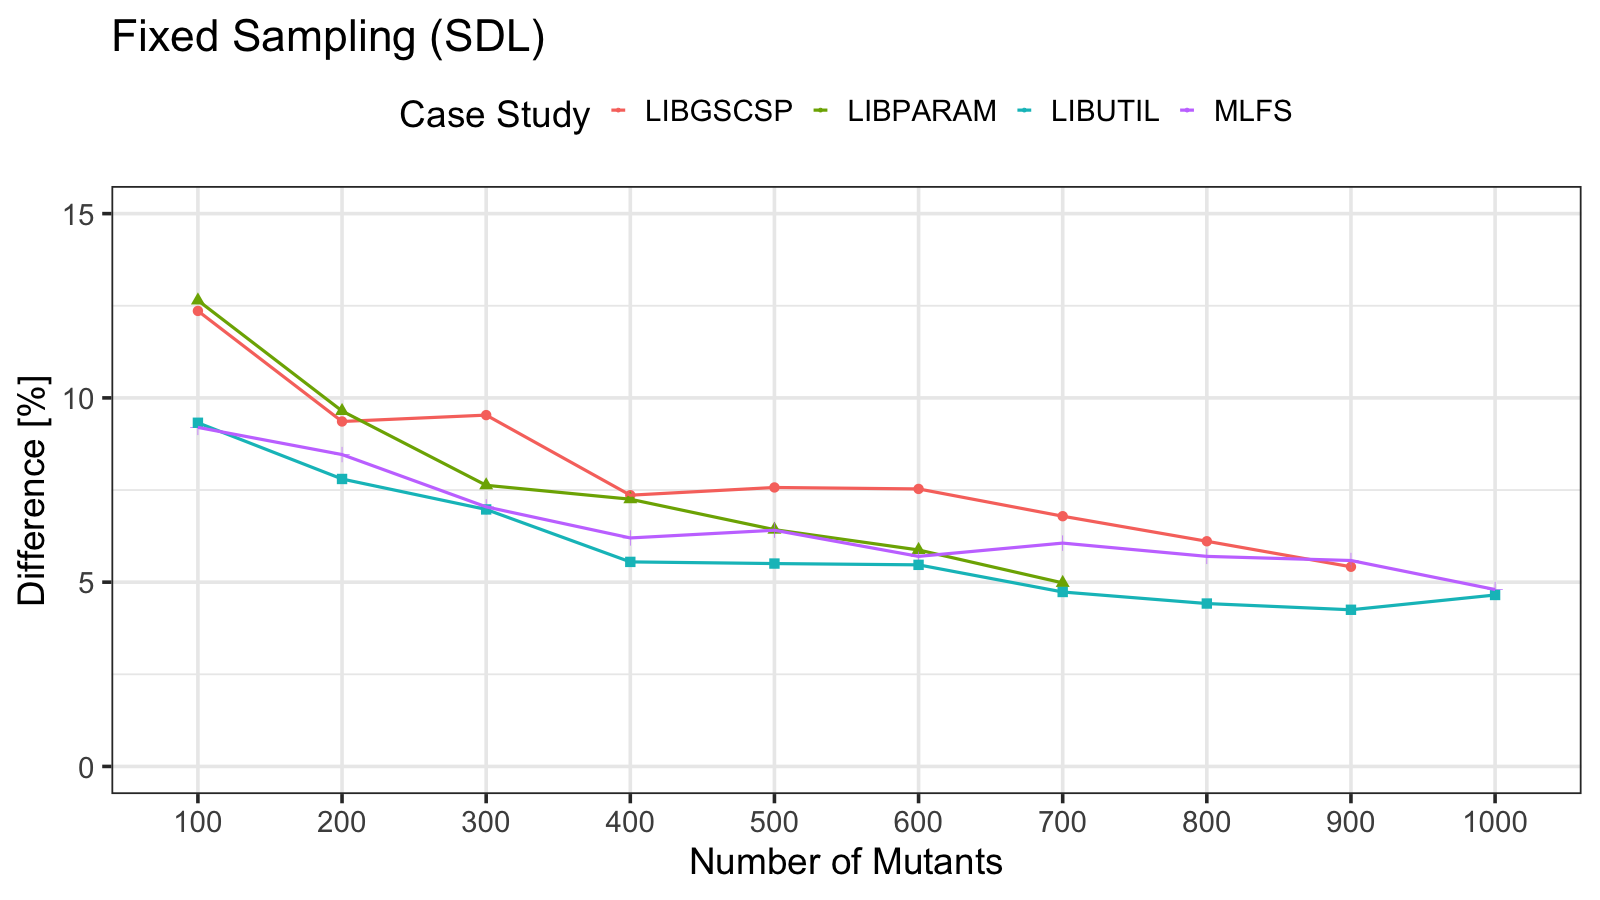
\includegraphics[width=6cm]{images/sampling_fixed_sdl}
%\caption{}
%\label{fig:results:fixedNumberOfMutantsSDL}
%\end{subfigure}
%\begin{subfigure}{.33\textwidth}
%  \centering
%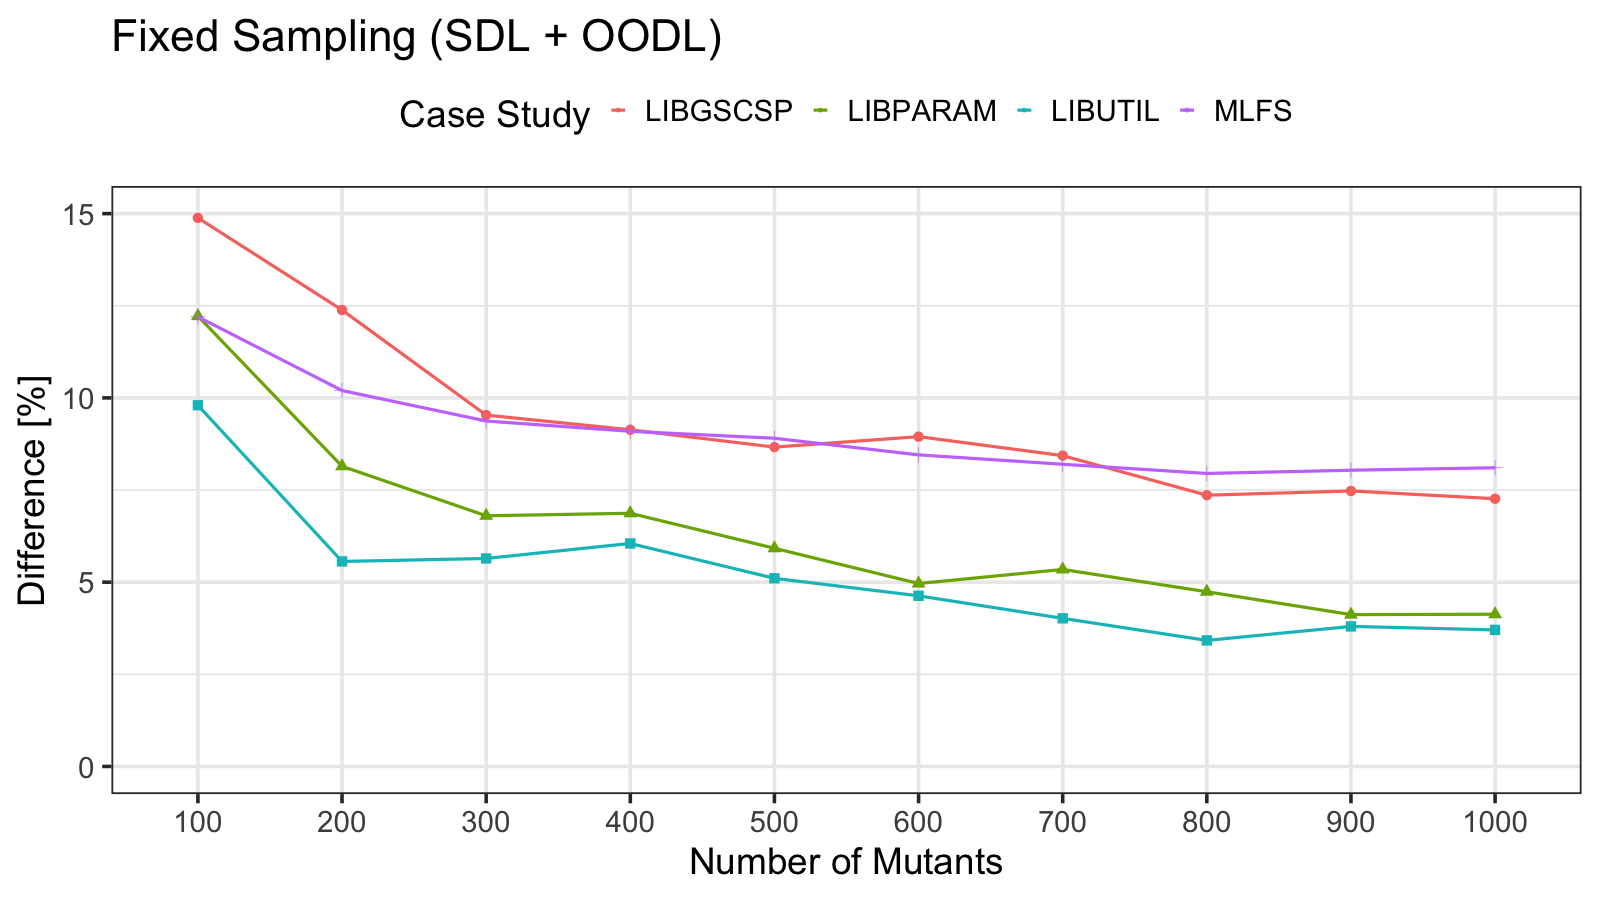
\includegraphics[width=6cm]{images/sampling_fixed_sdl_oodl}
%\caption{}
%\label{fig:results:fixedNumberOfMutantsSDLOODL}
%\end{subfigure}
%\begin{subfigure}{.33\textwidth}
%  \centering
%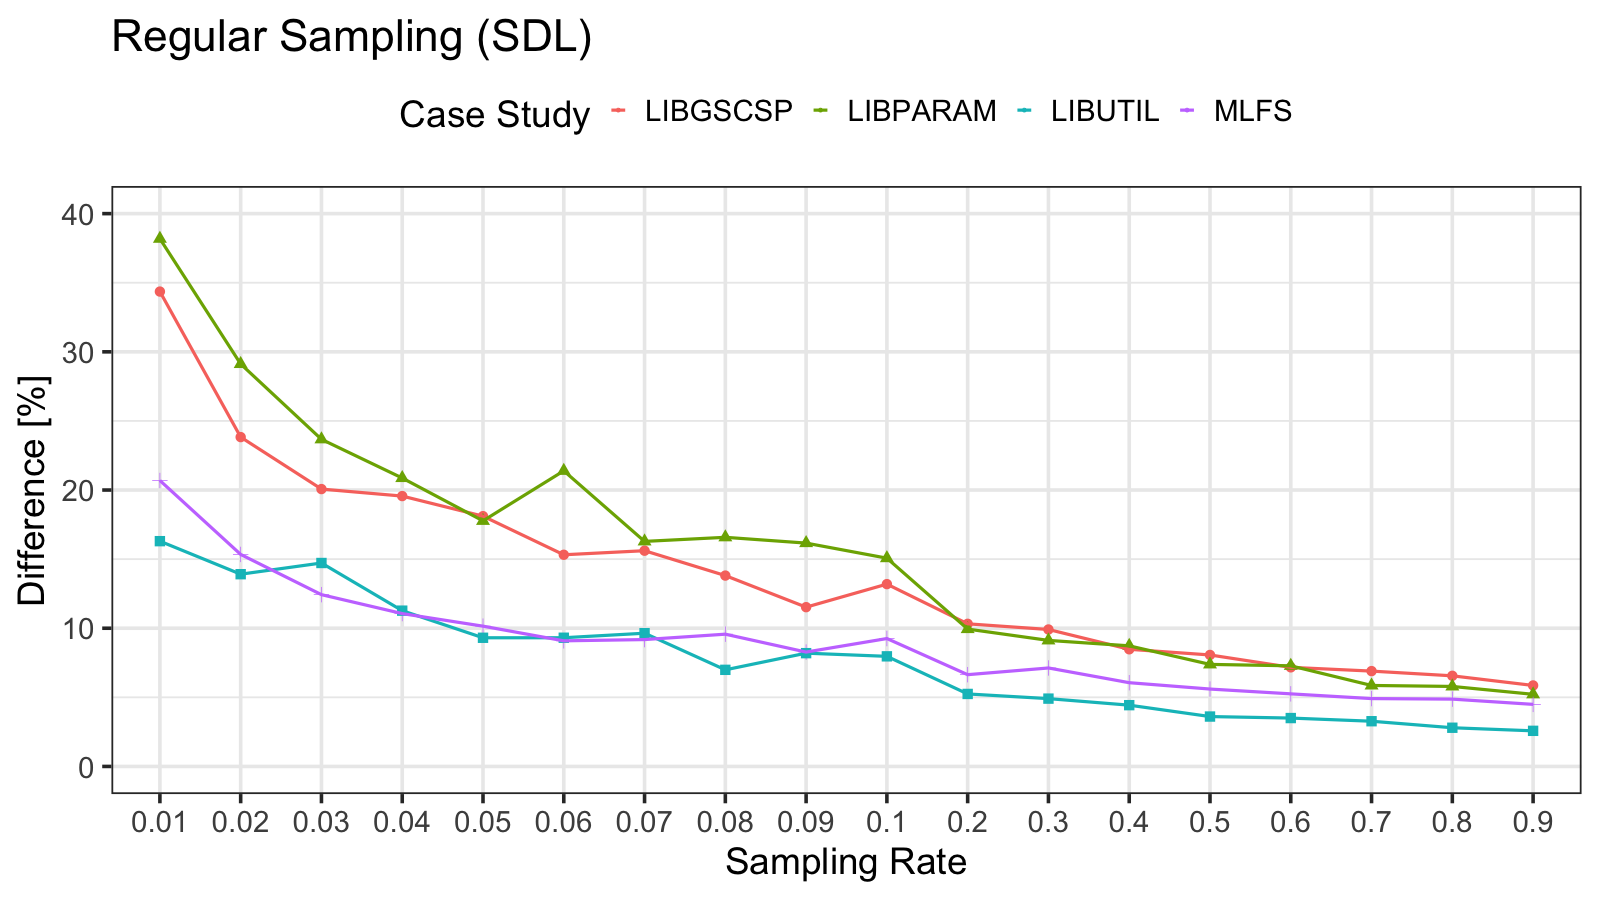
\includegraphics[width=6cm]{images/sampling_reg_sdl}
%\caption{}
%\label{fig:results:regNumberOfMutantsSDL}
%\end{subfigure}
%\begin{subfigure}{.33\textwidth}
%  \centering
%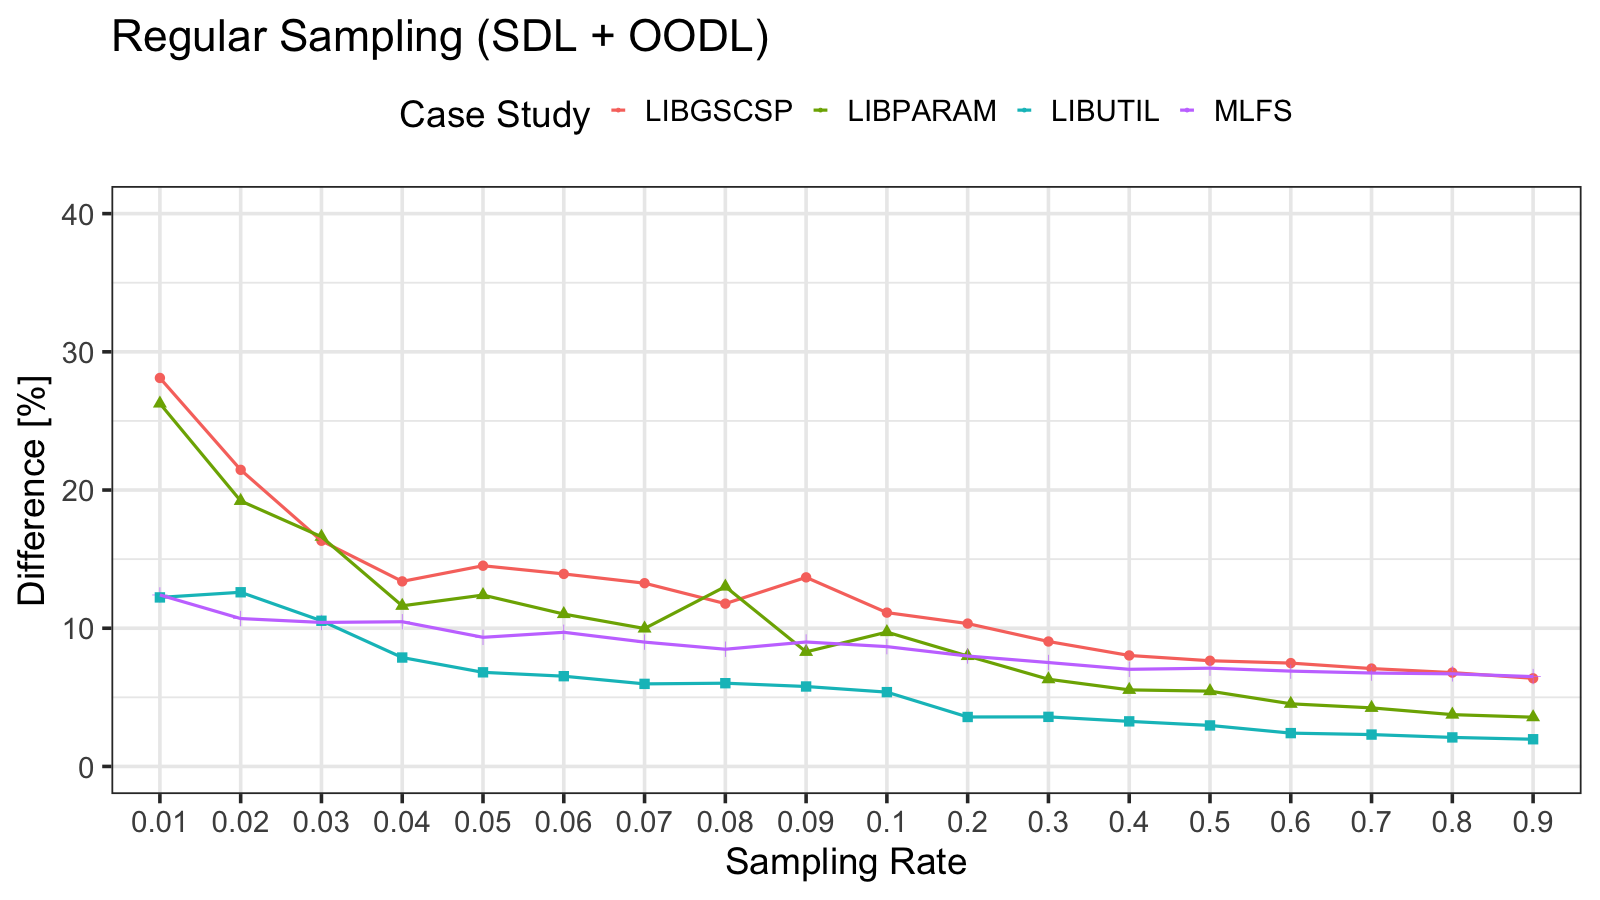
\includegraphics[width=6cm]{images/sampling_reg_sdl_oodl}
%\caption{}
%\label{fig:results:regNumberOfMutantsSDLOODL}
%
%\end{subfigure}
%\begin{subfigure}{.33\textwidth}
%  \centering
%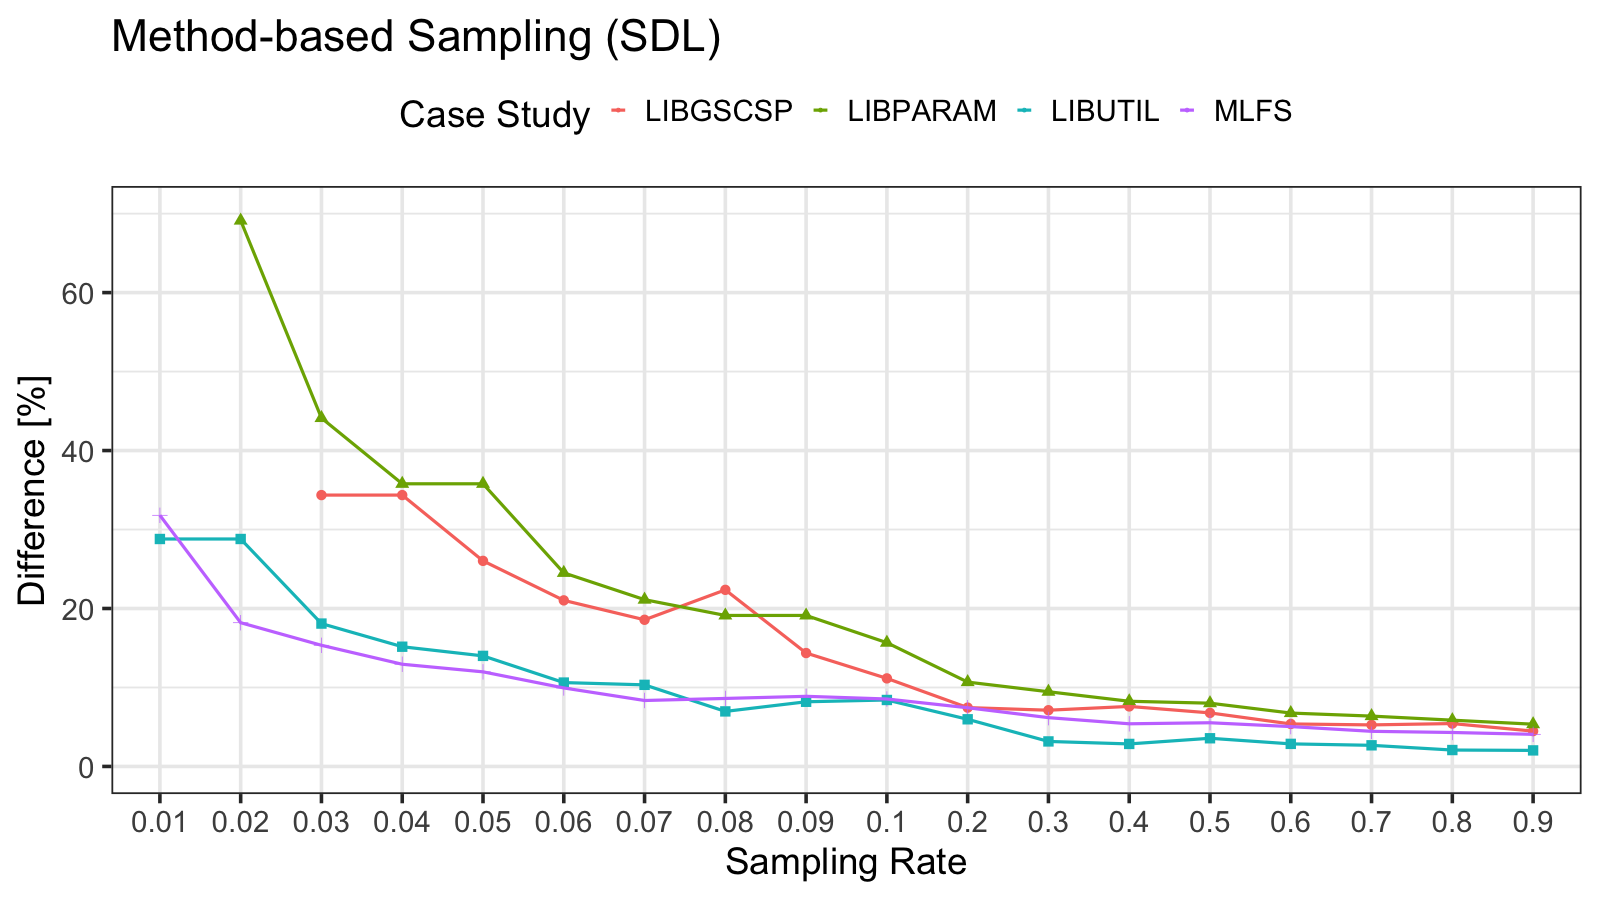
\includegraphics[width=6cm]{images/sampling_func_sdl}
%\caption{}
%\label{fig:results:funcNumberOfMutantsSDL}
%
%\end{subfigure}
%\begin{subfigure}{.33\textwidth}
%  \centering
%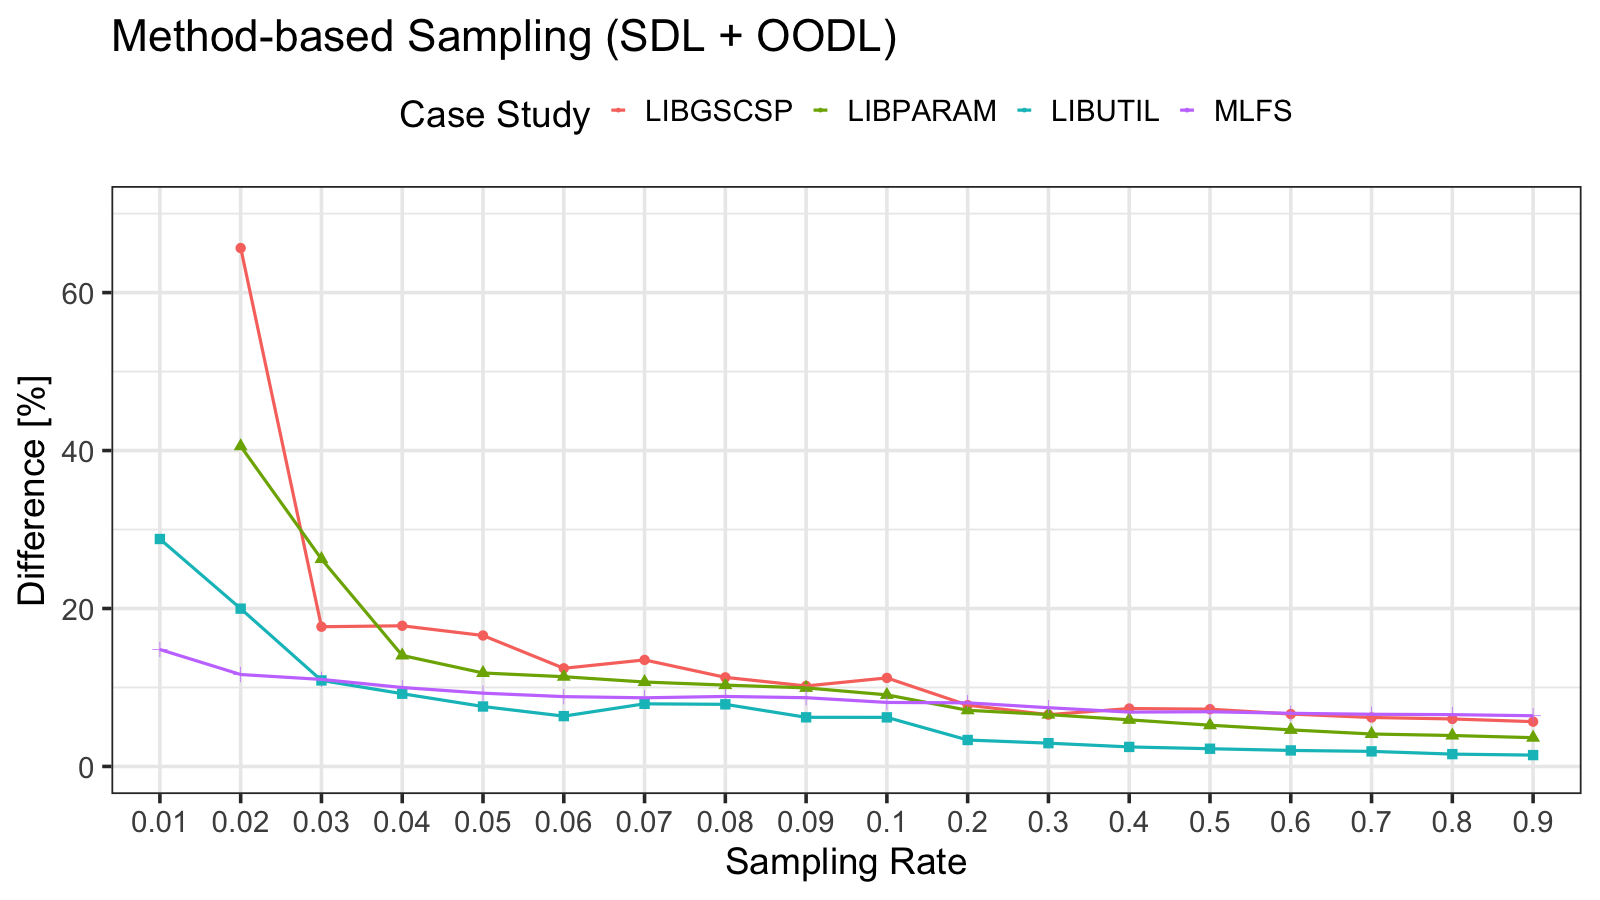
\includegraphics[width=6cm]{images/sampling_func_sdl_oodl}
%\caption{}
%\label{fig:results:funcNumberOfMutantsSDLOODL}
%
%\end{subfigure}
%\caption{}
%\label{fig:}
%\end{figure*}


\subsection{RQ4 - Mutation Score Accuracy with PrioritizeAndReduce}
\label{exp:accuracy:prioritize}

\paragraph{Design and measurements}

RQ4 assesses whether the mutation score obtained with the reduced and prioritized test suite generated by \APPR (hereafter, the \MPTS) accurately estimates the actual mutation  score.
%speeds up the mutation testing process.
To this end, we compare the accuracy obtained with the four distance metrics (i.e., $D_J$, $D_O$, $D_E$, and $D_C$) used by the proposed \INDEX{PrioritizeAndReduce} algorithm (Figure 1.6 from D2). In addition, to determine to what extent our prioritization strategy based on code coverage contributes to the selection of test cases that kill mutants, we also compare the results obtained with a simple baseline that, for each mutant, randomly selects one test case among the ones that cover the mutant. 


For all subjects, we consider (a) the complete set of mutants, (b) the reduced subset of mutants providing accurate results (i.e., the one obtained with FSCI sampling with $T_{\mathit{CI}}=0.10$). 
Based on RQ3 results, we exclude mutants generated with the SDL and SDL+OODL operators only. 
%Since, based on related work, engineers may still be interested in evaluating the mutation score obtained with SDL operators only, we study to what extent the test suite derived by the \emph{PrioritizeAndReduce} algorithm enable us to estimate the mutation score computed with the SDL operator.
For FSCI sampling, since we evaluate the accuracy of a reduced test suite, we derive the confidence interval using Equation 1.5 from D2. 
%Details about the estimated accuracy and number of mutants \ref{appendix:FSCI:reduced}.

%To the end of this research question, we study if the proposed reduction/prioritization strategies can produce a mutation score that is \textit{representative} with respect to the true mutation score obtained with no test suite reduction/prioritization strategies.

%We consider the same set of mutants as for RQ2.
For each subject and each distance metric, and for each of the two sets of mutants considered, we generated ten different \MPTSs. In the case of FSCI, since it randomly selects mutants, we considered ten different sets of mutants derived with distinct executions of the FSCI algorithm. For each \MPTS, we computed the mutation score obtained. 
Then, to determine if the mutation score of the \MPTS is accurate, we follow the same procedure adopted for RQ2, i.e., we rely on the 2.5/97.5 percentile distance from the actual mutation score. 
%In the case of the SDL set, we rely on the 2.5/97.5 percentile distance from the mutation score obtained with all the SDL mutants.



\paragraph{Results}

% !TEX root =  ../Main.tex

\begin{table}[]
\centering
\scriptsize
\caption{RQ4. Mutation score accuracy for the different strategies implemented by \emph{PrioritizeAndReduce}}
\label{table:results:PriritizeAndReduce} 
\begin{tabular}{|
p{15mm}@{\hspace{1pt}}|
p{15mm}@{\hspace{1pt}}|
>{\raggedleft\arraybackslash}p{15mm}@{\hspace{1pt}}|
>{\raggedleft\arraybackslash}p{15mm}@{\hspace{1pt}}|
>{\raggedleft\arraybackslash}p{15mm}@{\hspace{1pt}}|
}
\hline
           &          &\multicolumn{3}{c}{\textbf{$\delta_{acc}$}}\\
\hline
\textbf{Case Study} & \textbf{Strategy} & \textbf{ALL} & \textbf{FSCI (C=10)} & \textbf{SDL}  \\
\hline
\multirow{5}{*}{LIBUTIL}    
    & Random & 3.1400 & 5.87 & 3.5500  \\
           & $D_J$                    & 0.0300  & 2.54 & 0.0900  \\
           & $D_O$                    & 0.0300  & 2.54 & 0.0900  \\
           & $D_E$                    & 0.0199  & 2.51 & 0.0900  \\
           & $D_C$                    & 0.0199  & 2.57 & 0.0900 \\
\hline
\multirow{5}{*}{LIBGSCSP}   & Random & 7.2055 &  $>$5\% & 8.0605   \\
           & $D_J$                    & 1.3455  & 3.55 &1.5300 \\
           & $D_O$                    & 1.3100  & 3.55  &1.4200 \\
           & $D_E$                    & 0.7300  & 3.75  &0.6500 \\
           & $D_C$                    & 0.7300  & 3.75 &0.6500  \\
\hline
\multirow{5}{*}{LIBPARAM}   & Random & 7.7927 & $>$5\%  & 6.0892  \\
           & $D_J$                    & 0     &3.62& 0  \\
           & $D_O$                    & 0     &3.62& 0    \\
           & $D_E$                    & 0     &3.62& 0     \\
           & $D_C$                    & 0     &3.62& 0     \\
\hline
\multirow{5}{*}{MLFS}       & Random &  6.721  & $>$5\%   &    7.3999 \\
           & $D_J$                      &   0.3299   & 4.07&    0.2299    \\
           & $D_O$                      &   0.3299   & 4.07&     0.2299   \\
           & $D_E$                      &   0.0199   & 4.33&     0  \\
           & $D_C$                      &    0.0300  & 4.27&     0   \\
\hline
\multirow{5}{*}{ESAIL}      & Random & 38.8885      &   $>$5\%    &   39.1765\\
                                                & $D_J$      & 24.1688      &   $>$5\%     &  21.6800\\
                                                & $D_O$     & 24.3650      &  $>$5\%     &   21.7570\\
                                                & $D_E$     &  4.0800     &  4.7794     &   4.1400\\
                                                & $D_C$     &  3.9833    &   4.8825    &  4.5600\\
\hline
\end{tabular}
\end{table}


% \begin{table}[h]
% \centering
% \tiny
% \caption{RQ6. MS Comparison with respect to Random approach.}
% \label{table:results:msReducedRandomPVals} 
% \begin{tabular}{|llll|}
% \hline
% \textbf{Case Study}                & \textbf{\begin{tabular}[c]{@{}l@{}}MS Comparison\\w.r.t. Random\end{tabular}} & \textbf{ALL P-value} & \textbf{SDL P-value} \\
% \hline
% \multirow{4}{*}{LIBGSCSP} & $D_J$    & 1.47E-04     & 1.37E-04 \\
%                           & $D_O$    & 1.40E-04     & 1.19E-04  \\
%                           & $D_E$    & 5.18E-05     & 5.30E-05  \\
%                           & $D_C$    & 1.17E-04     & 1.08E-04  \\
% \hline
% \multirow{4}{*}{LIBUTIL}  & $D_J$    & 1.27E-04      & 1.23E-04 \\
%                           & $D_O$    & 1.20E-04      & 1.15E-04 \\
%                           & $D_E$    & 1.20E-04      & 1.15E-04  \\
%                           & $D_C$    & 1.31E-04      & 1.26E-04 \\
% \hline
% \multirow{4}{*}{LIBPARAM} & $D_J$    & 5.38E-05      & 4.96E-05 \\
%                           & $D_O$    & 5.38E-05      & 4.96E-05 \\
%                           & $D_E$    & 5.38E-05      & 4.96E-05 \\
%                           & $D_C$    & 5.38E-05      & 4.96E-05 \\
% \hline
% \multirow{4}{*}{MLFS}     & $D_J$    &  1.40E-04    &  5.30E-05\\
%                           & $D_O$    &  1.40E-04      & 5.30E-05 \\
%                           & $D_E$    &  1.36E-04      &5.30E-05 \\
%                           & $D_C$    &  1.48E-04      & 5.30E-05 \\
% \hline
% \multirow{4}{*}{ESAIL}    & $D_J$    &                \\
%                           & $D_O$    &                \\
%                           & $D_E$    &                \\
%                           & $D_C$    &               \\
% \hline
% \end{tabular}
% \end{table}



%\begin{table*}
%\tiny
%\centering
%\caption{RQ6. P-value comparison between test suite reduction approaches.}
%\label{table:results:pValComparisonTSredPrior} 
%\begin{tabular}{|l|l|lllll|l|lllll|}
%\hline
%           &          & ALL      &                       &                       &          &      &          & SDL      &                       &                       &                       &       \\
%\hline           
%Case Study &          & Random & $D_J$                  & $D_O$                  & $D_E$     & $D_C$ &          & Random & $D_J$                  & $D_O$                  & $D_E$                  & $D_C$  \\
%\hline
%LIBGSCSP   & Random &          &                       &                       &          &      & Random &          &                       &                       &                       &       \\
%           & $D_J$     & 1.47E-04 &                       &                       &          &      & $D_J$     & 1.37E-04 &                       &                       &                       &       \\
%           & $D_O$     & 1.40E-04 & 2.50E-01              &                       &          &      & $D_O$     & 1.18E-04 & 7.88E-02              &                       &                       &       \\
%           & $D_E$     & 5.18E-05 & 5.15E-05              & 4.81E-05              &          &      & $D_E$     & 5.30E-04 & 4.56E-04              & 3.80E-05              &                       &       \\
%           & $D_C$     & 1.17E-04 & 1.16E-04              & 1.10E-04              & 2.93E-02 &      & $D_C$     & 1.08E-04 & 9.55E-05              & 8.21E-05              & 6.71E-02              &       \\
%\hline
%LIBUTIL    & Random &          &                       &                       &          &      & Random &          &                       &                       &                       &       \\
%           & $D_J$     & 1.27E-04 &                       &                       &          &      & $D_J$     & 1.23E-04 &                       &                       &                       &       \\
%           & $D_O$     & 1.20E-04 & 8.31E-01              &                       &          &      & $D_O$     & 1.15E-04 & 8.31E-01              &                       &                       &       \\
%           & $D_E$     & 1.20E-04 & 8.38E-03              & 2.05E-03              &          &      & $D_E$     & 1.15E-04 & 8.31E-01              & \multicolumn{1}{r}{1} &                       &       \\
%           & $D_C$     & 1.31E-04 & 6.40E-03              & 2.20E-03              & 5.34E-01 &      & $D_C$     & 1.26E-04 & 6.80E-01              & 5.34E-01              & 5.34E-01              &       \\
%\hline
%LIBPARAM   & Random &          &                       &                       &          &      & Random &          &                       &                       &                       &       \\
%           & $D_J$     & 5.38E-05 &                       &                       &          &      & $D_J$     & 4.96E-05 &                       &                       &                       &       \\
%           & $D_O$     & 5.38E-05 & \multicolumn{1}{r}{1} &                       &          &      & $D_O$     & 4.96E-05 & \multicolumn{1}{r}{1} &                       &                       &       \\
%           & $D_E$     & 5.38E-05 & \multicolumn{1}{r}{1} & \multicolumn{1}{r}{1} &          &      & $D_E$     & 4.96E-05 & \multicolumn{1}{r}{1} & \multicolumn{1}{r}{1} &                       &       \\
%           & $D_C$     & 5.38E-05 & \multicolumn{1}{r}{1} & \multicolumn{1}{r}{1} &    \multicolumn{1}{r}{1}   &      & $D_C$     & 4.96E-05 & \multicolumn{1}{r}{1} & \multicolumn{1}{r}{1} & \multicolumn{1}{r}{1} &       \\
%\hline
%MLFS       & Random &          &                       &                       &          &      & Random &          &                       &                       &                       &       \\
%           & $D_J$     & 1.40E-04 &                       &                       &          &      & $D_J$     & 5.30E-05 &                       &                       &                       &       \\
%           & $D_O$     & 1.40E-04 & \multicolumn{1}{r}{1} &                       &          &      & $D_O$     & 5.30E-05 & \multicolumn{1}{r}{1} &                       &                       &       \\
%           & $D_E$     & 1.36E-04 & 1.20E-04              & 1.20E-04              &          &      & $D_E$     & 5.30E-05 & 1.31E-05              & 1.31E-05              &                       &       \\
%           & $D_C$     & 1.48E-04 & 1.31E-04              & 1.31E-04              & 1.61E-02 &      & $D_C$     & 5.30E-05 & 1.31E-05              & 1.31E-05              & \multicolumn{1}{r}{1} &       \\
%\hline
%ESAIL      & Random &          &                       &                       &          &      & Random &          &                       &                       &                       &       \\
%           & $D_J$     &          &                       &                       &          &      & $D_J$     &          &                       &                       &                       &       \\
%           & $D_O$     &          &                       &                       &          &      & $D_O$     &          &                       &                       &                       &       \\
%           & $D_E$     &          &                       &                       &          &      & $D_E$     &          &                       &                       &                       &       \\
%           & $D_C$     &          &                       &                       &          &      & $D_C$     &          &                       &                       &                       &      \\
%\hline           
%\end{tabular}
%\end{table*}




Table~\ref{table:results:PriritizeAndReduce} provides the values of $\delta_{acc}$ obtained for the different subjects and distance metrics (i.e., the random baseline and the four distance metrics supported by \APPR). Rows named \emph{ALL} report the results obtained when executing the entire set of mutants, rows named \emph{FSCI}  report the results obtained  with the FSCI strategy. 
%column \emph{SDL} reports the results for the mutants generated with the SDL operator only.



\NEWFSCI{Unsurprisingly, for all the subjects except \SAIL{}$_S$, the mutation score computed with the entire set of mutants tested with the \MPTS (i.e., row ALL) is more accurate than the mutation score computed with a subset of the mutants tested with the same test suite (i.e., row FSCI). 
%However, the distance metrics $D_E$ and $D_C$ enable the accurate estimation (i.e, $\delta_{acc}  < 5$) of the actual mutation score with FSCI.
However, the mutation score estimated with FSCI is always accurate (i.e, $\delta_{acc}  < 5$).
In the case of \SAIL{}$_S$, where each statement is covered by a large number of test cases (see Section~\ref{sec:empirical:subjects}),
%\footnote{\UPDATE{In $ESAIL_S$, each statement is covered on average by 61 test cases. In the other cases, each statement is covered by 2 test cases, on average (see Section~\ref{sec:empirical:subjects}).}}, 
test suite reduction has a higher probability of retaining a test case that does not kill a mutant.
For this reason, executing a reduced test suite with a subset of mutants selected with FSCI, which estimates the error due to test suite reduction, 
leads to a more accurate mutation score than executing a reduced test suite with the entire set of mutants without estimating such error (i.e., row ALL).
%For this reason, FSCI, which estimates the error due to test suite reduction, 
%performs better.
% than the execution of the entire set of mutants without estimating such error (i.e., row ALL).
%FSCI enables a more accurate computation of the mutation score for the \MPTS. 
%\FIXME{It happens because estimation errors due to test suite reduction are minimal
%\footnote{Figure~\ref{} shows that the number of test cases executed by FSCI with the whole test suite is similar to the one with the reduced test suite}, consequently 
%enforcing $|\mathit{CI}_E| \le T_{\mathit{CE}}$ simply augment the sample size thus improving the accuracy of the estimation.}
}

%enforcing PKErr, which is used to compute a corrected confidence interval and consequently the mutation score. The corrected confidence interval, which takes into account PKErr enable us to obtain a more accurate mutation score than the one computed with the whole test suite. Which is an additional reason for adopting FSCI.}}
 

%% Comment 25/02/2021:
%% In the case of ESAIL, the higher delta is likely due to the large number of test cases covering each mutant, which increases the likelihood of removing  test cases that kill the mutant. Consequently, the mutation score may be affected. In the case of FSCI, such error in the computation score is estimated with the initial tuning to estimate PKErr, which is used to compute a corrected confidence interval and consequently the mutation score. The corrected confidence interval, which takes into account PKErr enable us to obtain a more accurate mutation score than the one computed with the whole test suite. Which is an additional reason for adopting FSCI.
%% For reviewer: we realized with additional experiments, that the updated procedure lead to a mutation score that is more accurate than the mutation score computed with the whole set of mutants.


The only distance metric that consistently leads to inaccurate estimates of the mutation score (i.e., $\delta_{acc}  > 5$) across subjects is the random baseline.
Based on a non-parametric Mann Whitney test, the difference between the random baseline (i.e., Random) and the four distance metrics implemented by \APPR (i.e., $D_*$) is always significant with a \textit{p}-value $< 0.05$. This indicates that \textbf{the \APPR distance metrics are necessary to accurately estimate the mutation score while reducing the number of test cases to  execute}.

Among the proposed distance metrics, 
$D_J$ and $D_O$ provide inaccurate results with \SAIL{}$_S$.
%and less accurate results for other subjects than alternatives. 
We conjecture the main reason is their inability to account for the number of times a statement is exercised by a test case. 
We believe this is an important factor as system test cases that repeatedly exercise mutated statements, with different variable values, are more likely to kill mutants than test cases exercising such statements only once (e.g., because of the uncertainty regarding the 
\JMR{3.16}{incorrect intermediate state
%infected program state
propagating to the state variables verified by test oracles, see Section~1.2.1.1 from D2}). On the other hand, unit and integration test cases, which exercise much simpler scenarios in other subjects, are more likely to kill a mutant when the mutated statement is executed only once (e.g., because the oracle is closer to the mutated statement). This is why $D_J$ and $D_O$ fare similarly to the other distance metrics for these subjects. 
%Almost every system test case exercises certain components (e.g., the handler of telecommands, which is the main entry point of the system) but only the ones executing such components repeatedly (e.g., to verify multiple combination of input values for a same telecommand) carefully exercise mutated statements. Regarding the other subjects, each unit and integration test case rather tends to focus on simple test scenarios that exercise mutated statements once or a few times.
In contrast, $D_C$ and $D_E$ are distance metrics ensuring an accurate estimate of the mutation score and providing the lowest $\delta_{acc}$. The differences between $D_E$ and $D_C$ are always statistically significant, \UPDATE{except for \MLFS{}{}}. However, there are no practically significant differences between them. 
Since $D_C$ provides a normalized score, which is required by Step 8, we select $D_C$ as the preferred metric to be used in \APPR.
%the Based on $\delta_{acc}$, the metric that perform slightly better is $D_E$ (the sum of the $\delta_{acc}$ across all the case studies for all the configurations is lower than for $D_E$. \textbf{We thus select $D_E$ as the best metric to be used with \APPR}.


\subsection{RQ5 - Time Savings with PrioritizeAndReduce}

\paragraph{Design and measurements}

RQ5 assesses to what extent  the \MPTS speeds up the mutation analysis process.


For each subject considered for RQ4, we measure the execution time taken by the \MPTS to execute on the mutants.
We compute time saving as the ratio of the difference in execution time from the original test suite over the time it requires to execute, for the set of mutants selected.
In particular, as in RQ4, we consider three scenarios (1) all the mutants are selected, (2) mutants are selected with FSCI sampling, (3) mutants are selected with FSCI sampling but we execute the entire test suite, as opposed to the \MPTS. By considering scenario (3), we can estimate both the time saved thanks to mutant sampling and the additional time saved when combining it with the \MPTS.
For the original test suite, to emulate a realistic mutation analysis process according to state-of-the-art solutions, we measure the time required to execute test cases until the mutant is killed (for live mutants it means that we execute the entire test suite). Also, we set a test case timeout equal to three times the duration of the original test case.

Since the execution time of test cases depends on multiple factors such as the underlying test harness, the development practices in place (e.g., verifying multiple scenarios in a single test case), and the type of testing conducted (e.g., unit, integration, system), we also compute 
the ratio of the number of test cases not executed by the \MPTS over the total number of test cases.

\paragraph{Results}

Table~\ref{table:time:original} reports, for every subject, the time required to test all the mutants with the entire test suite, in seconds. It also reports  the total number of test cases executed. 
We observe that mutation analysis requires a large amount of time. It takes between 13 and 73 hours for subjects tested with unit and integration test suites (which are faster to execute). When a system test suite needs to be executed (i.e., $\mathit{\SAIL{}_S}$), traditional mutation analysis becomes infeasible as shown by the 11,000 hours required to perform mutation analysis with $\mathit{\SAIL{}_S}$.

Figures~\ref{fig:results:time:saving} and~\ref{fig:results:test:saving} provide boxplots depicting 
the saving achieved when the \MPTS is executed with all the mutants and with the FSCI-selected mutants, in terms of execution time and test cases, respectively. Each observation corresponds to the saving obtained with one of the ten executions performed on each subject, for a specific configuration (i.e., distance $D_*$ and strategy adopted for selecting mutants). In Figures~\ref{fig:results:time:saving} and~\ref{fig:results:test:saving}, horizontal dashed lines show the average across all subjects, whiskers are used to identify outliers (i.e., they are placed below/above 1.5*Inter Quartile Range of the upper quartile/lower quartile). A detailed table including min, max, mean, and median values for each subject is provided in Appendix C.
%~\ref{appendix:details:rq5}.

%Table~\ref{table:results:reduction:prioritize} reports the saving achieved when the \APPR test suite is executed with all the mutants, with the FSCI selected mutants, with the SDL mutants. For both time savings and test savings, we report the min, max, median, and mean values. Values are reported for all the case studies, for all the distance metrics, and for the three strategies considered to select mutants (i.e., selecting all the available mutants, selecting all the mutants generated with the SDL operator, and selecting mutants with the FSCI strategy).

Unsurprisingly, the smallest reduction in execution time and number of executed test cases is achieved when executing the \MPTS with all the mutants. 
Measuring such time reduction allows us to evaluate the benefits of test suite prioritization and selection when it is not combined with mutant selection.
Excluding outliers, execution time reduction goes from  \UPDATE{-0.52\%} % -0.11\% was the 1st quantile not the whisker
to 16.82\% and appears to be correlated with the reduction in number of test cases to execute, which varies from 4.80\% to 33.17\%.
The largest reductions are obtained with $D_J$ and $D_O$ (the median is 13.36 and 13.40, respectively), which do not consider differences in coverage frequency, thus removing the largest number of test cases; however, $D_J$ and $D_O$ also lead to the worst accuracy results according to RQ4. Metrics $D_C$ and $D_E$, instead, lead to limited benefits in terms of time reduction.

A negative reduction indicates that the reduced and prioritized test suite increases the execution time of the mutation analysis process. This happens when (1) test cases are sorted in such a way that test cases that kill the mutants are executed later with respect to the original test suite, (2) test cases that kill the mutants but have long execution times (e.g., because they trigger a timeout) are executed before test cases with shorter execution times that kill the mutants. Negative reduction, however, affects only a few executions, thus showing that a reduced and prioritized test suite tends overall to be beneficial to the mutation analysis process.



%With our subject artifacts, in terms of execution time, test suite prioritization is thus not always beneficial; however, it always lead to a reduction the number of test cases between 4.82 and 33.15. The distance metrics leading to the highest reduction in the number of test cases are $D_J$ and $D_O$, i.e., the ones with the lowest accuracy computed for RQ 4.

Mutant sampling alone contributes to a high reduction in execution time; indeed, in Figure~\ref{fig:results:time:saving}, the boxplot \emph{FSCI 0.1-Full TS}, depicting the time saving for FSCI mutants tested with the entire test suite, shows minimum, median, and maximum values of 65.76\%, 75.10\%, and 84.72\%. Indeed, by reducing the number of mutants to execute, FSCI sampling significantly reduced the total number of test cases to execute within a [\JMRCHANGE{49.98\%} - 80.54\%] range (as shown by the boxplot in Figure~\ref{fig:results:test:saving}).

The highest reduction in execution time is achieved when combining the \MPTS with FSCI sampling. It ranges from 72.09\% to 90.83\%. $D_C$ and $D_E$, which are the approaches that guarantee accurate results, lead to an execution time reduction in the ranges \JMRCHANGE{[75.25\% - 90.83\%]} and \JMRCHANGE{[73.53\% - 90.83\%]}, respectively, an impressive achievement. 
Test case savings, 
%show similar ranges, 
\JMRCHANGE{as well, are above 65\%, [68.28\% - 83.45\%]} and \JMRCHANGE{[68.08\% - 82.70\%]} for $D_C$ and $D_E$, respectively. Based on savings results, there is no practical difference between $D_C$ and $D_E$.

%The number of test cases being executed is reduced by 84.50\% for $D_J$ and $D_O$ and by 84.08\% for $D_E$ and $D_C$. When combined with FSCI sampling the differences between the different distance metrics are thus not practically significant (27 minutes, in total, across all the case studies), the selection of the coverage distance metric $D_*$ can thus rely on RQ4 results.

To conclude, \textbf{we suggest to combine FSCI sampling with the \MPTS to minimize the time required by mutation analysis}. 
For $\mathit{\SAIL{}}_S$, 
\NEWFSCI{on average, when combining the \MPTS with FSCI sampling, mutation analysis time goes from 11,000 hours to 1,531 hours, which makes mutation analysis feasible in one week with 10 computing nodes.} Note that for safety or mission critical systems, such as satellites software, the cost of using computing nodes is minimal compared to the development cost of the entire system. Indeed, to test such systems, even paying for the computational power of 100 HPC nodes to make mutation analysis feasible in half a day, is economically justifiable. \JMR{2.2}{Otherwise, without \APPR, mutation analysis leads to 11,000 hours of test cases execution, thus being practically infeasible since it would require more than 100 days to be completed, even with 100 HPC nodes.}

Our results also show that when it is not feasible to collect coverage data for the mutants under test (a requirement to generate the \MPTS), \textbf{FSCI sampling alone, without a reduced test suite, may still provide a high reduction in execution time}. In the case of $\mathit{\SAIL{}}_S$, this leads to 2,920 mutation analysis hours, which require less than two days with 100 HPC nodes.

% !TEX root =  ../Main.tex

\begin{table}[tb]
\caption{Execution time and number of test cases executed when mutation testing is based on the original test suite.}
\label{table:time:original} 
\scriptsize
\begin{tabular}{|
p{12mm}@{\hspace{2pt}}|
>{\raggedleft\arraybackslash}p{44mm}@{\hspace{1pt}}|
>{\raggedleft\arraybackslash}p{12mm}@{\hspace{1pt}}|
}
\hline
\textbf{Component}&\multicolumn{1}{c|}{\textbf{Execution time}}&\multicolumn{1}{c|}{\textbf{\# Test cases}}\\
\hline
\multirow{1}{*}{ESAIL$_S$}& 39\,604\,457 seconds (~ 11\,000 hours) & 155\,751 \\
%& SDL& & \\
\hline
\multirow{1}{*}{LIBGSCSP}&  252776 seconds (~70 hours)& 10250\\
%& SDL& 53074& 2103\\
\hline
\multirow{1}{*}{LIBPARAM}&  47949 seconds (~13 hours)& 6629\\
%& SDL& 7321& 1269\\
\hline
\multirow{1}{*}{LIBUTIL}&  214016 seconds (~59 hours)& 17672\\
%& SDL& 37603& 3030\\
\hline
\multirow{1}{*}{MLFS}&  171790 seconds (~48 hours)& 28159\\
%& SDL& 13492& 2220\\
%MLFS$_V$& 31526 &T &28069&89.03\% &X\\
\hline
\textbf{Total}&   & \\ 
\hline
\end{tabular}
\end{table}

\begin{figure}[tb]
\begin{center}
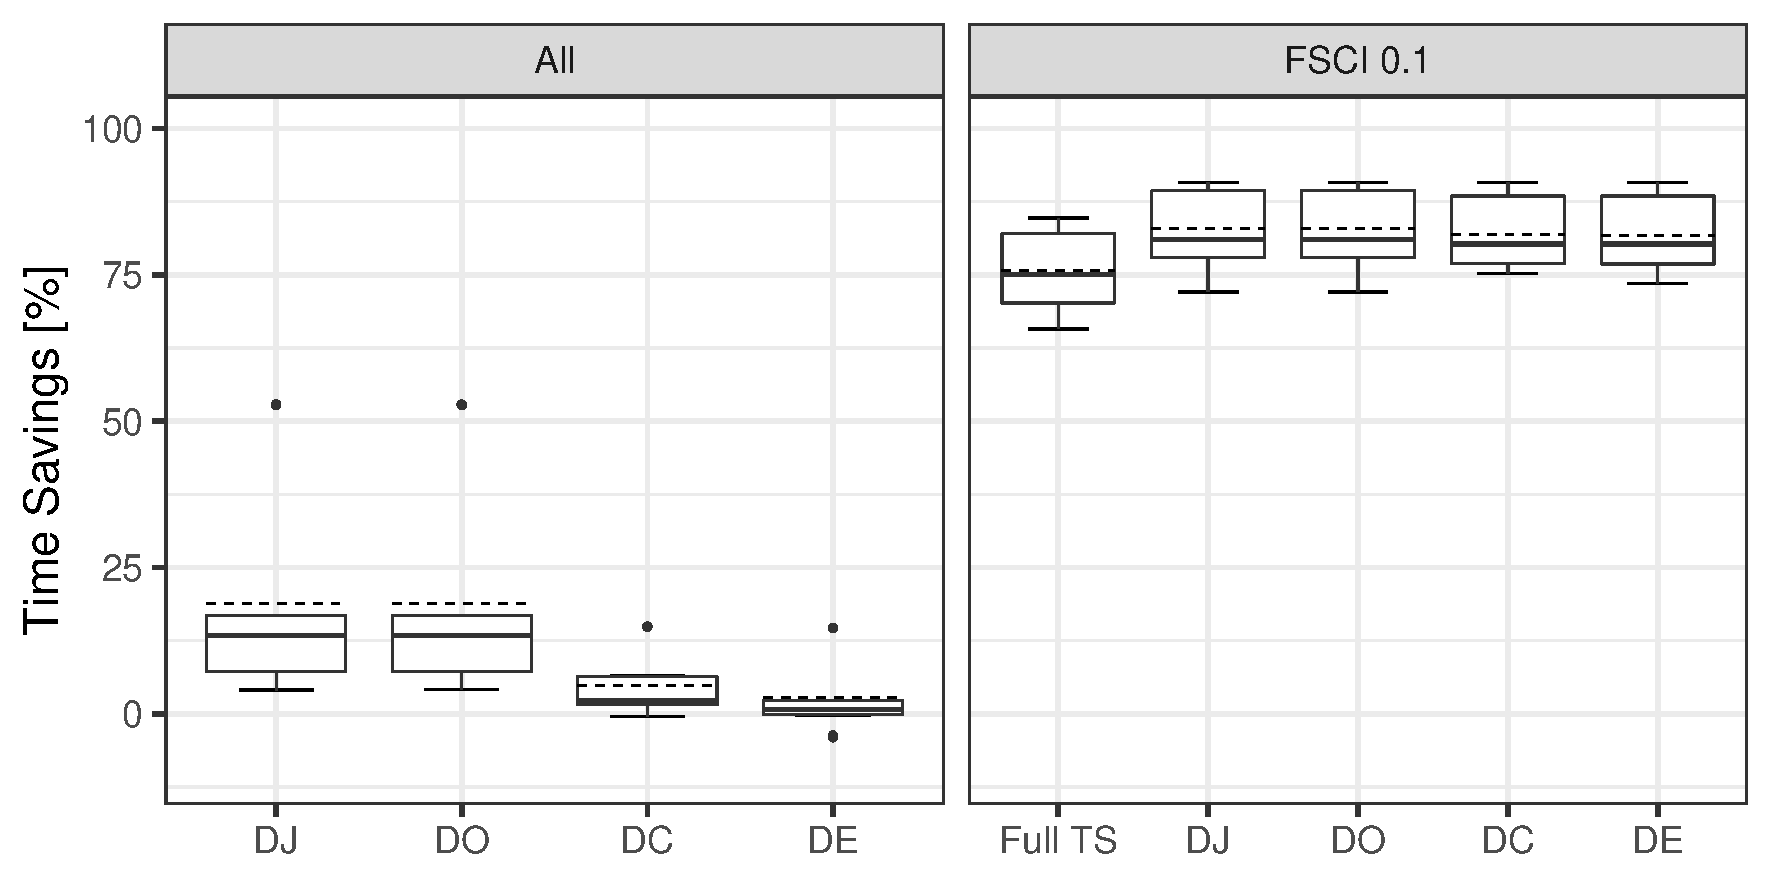
\includegraphics[width=0.8\columnwidth]{images/times.pdf}
\caption{Time savings for different sets of mutants, with the \MPTS being generated based on different distance measures.}
\label{fig:results:time:saving}
\end{center}
\end{figure}

\begin{figure}[tb]
\begin{center}
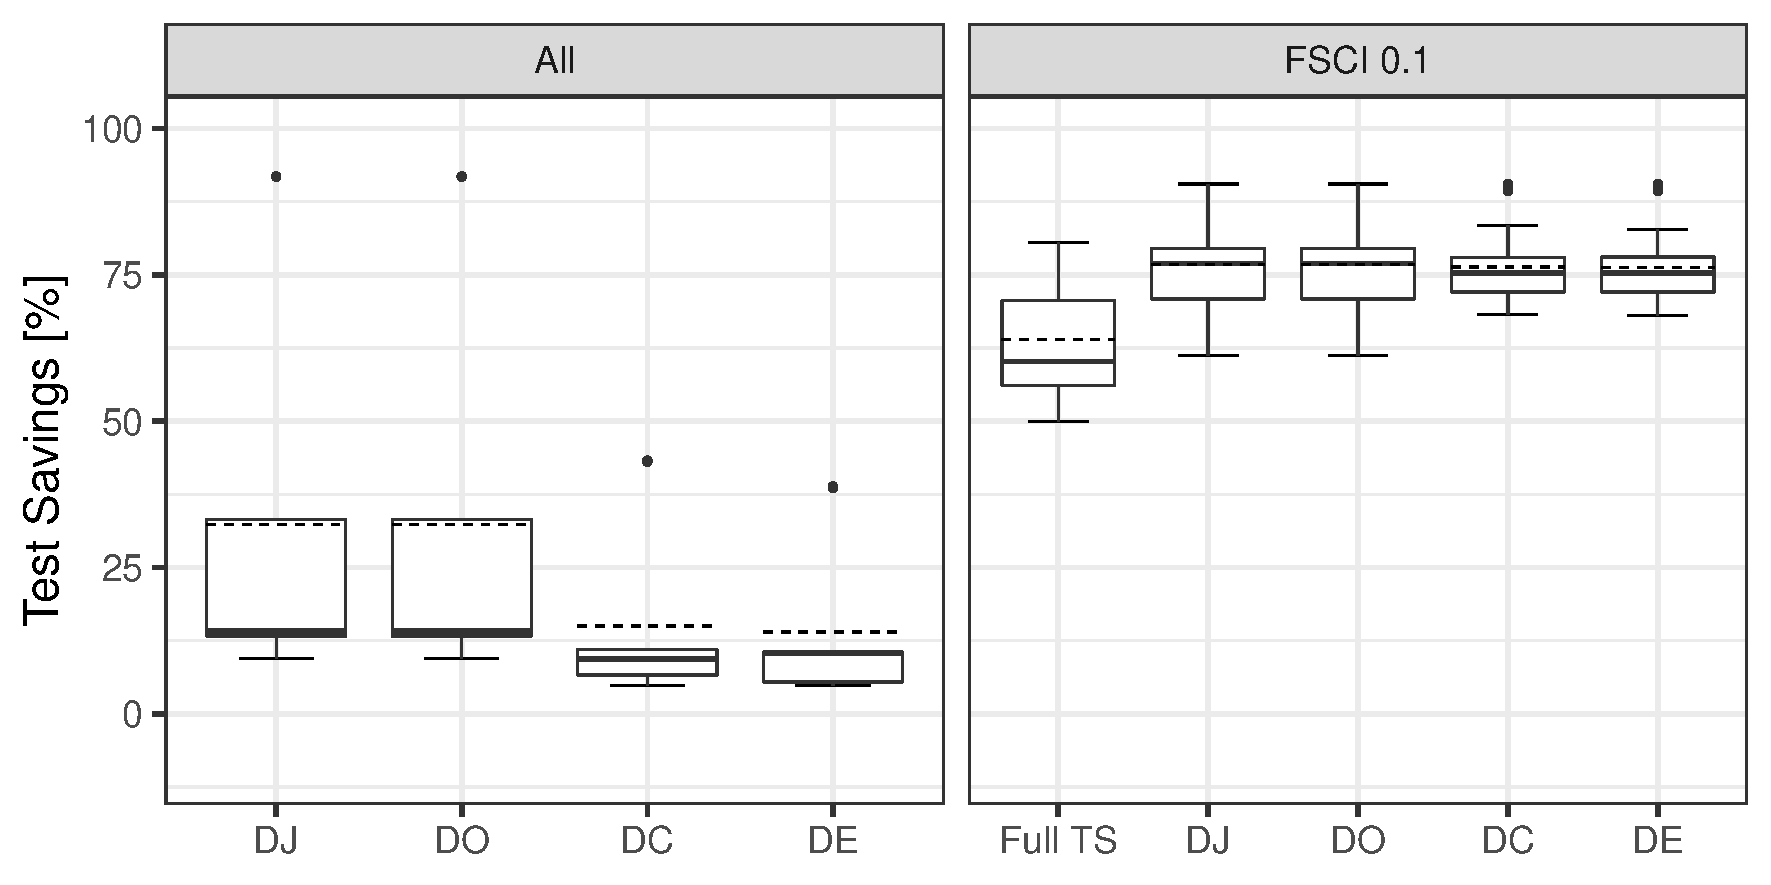
\includegraphics[width=0.8\columnwidth]{images/tests.pdf}
\caption{Test case savings for different sets of mutants, with the \MPTS being generated based on different distance measures.}
\label{fig:results:test:saving}
\end{center}
\end{figure}




\subsection{RQ6 - Precise Detection of Equivalent and Duplicate Mutants}
\label{sec:empirical:thrshold}
\paragraph{Design and measurements}
RQ6 investigates if it is possible to identify thresholds that enable the accurate identification of mutants that are nonequivalent ($T_E$) and nonduplicate ($T_D$), following the procedure described in Section 1.2.3.7 from D2.

To determine $T_E$ and $T_D$, 
we rely on the optimal distance metric identified in RQ4 ($D_C$).
%for each normalized distance metric ($D_J$, $D_O$, $D_E$, $D_C$), 
We analyze  precision and recall of the results obtained for  different values of $T_E$ and $T_D$.
%being equal to $0.0$, between $0.0$ and $0.4$,  between $0.4$ and $0.8$, between $0.8$ and $1$.
%\CHANGED{We do not discuss recall (i.e., the percentage of equivalent mutants detected by our approach) since it is not feasible to compute the overall number of equivalent, live mutants. Indeed, it would imply manually inspecting all the live mutants, 12,330 in total, across all subjects (see Table~\ref{table:results:accuracy:full}).}
%being equal to $0.0$, $0.4$, and $0.8$.
To determine $T_E$, we measure
precision as the percentage of mutants with a distance above $T_E$ that are nonequivalent, recall as the percentage of nonequivalent mutants with a distance above $T_E$.
To determine $T_D$, we measure
precision as the percentage of mutant pairs with a distance above $T_D$ that are duplicate, recall as the percentage of duplicate mutant pairs that have a distance above $T_D$.
%\CHANGED{We do not discuss recall (i.e., the percentage of equivalent mutants detected by our approach) since it is not feasible to compute the overall number of equivalent, live mutants. Indeed, it would imply manually inspecting all the live mutants, 12,330 in total, across all subjects (see Table~\ref{table:results:accuracy:full}).}

Since the quality of results might be affected by both test suite reduction (i.e., less coverage data may be available) and mutants sampling (e.g., less mutants might be sampled), consistent with the finding of previous RQs, we consider the following two configurations: 
\begin{itemize}
\item Execution of the original test suite with all the generated mutants (ALL)
%\item Execution of the original test suite against a random selection of x\% mutants
%\item Execution of the original test suite against a random selection of x\% SDL mutants
%the following might become model-based
%\item Execution of the \APPR test suite with a random selection of x\% mutants
\item Execution of the \MPTS with FSCI sampling (\APPR)
\end{itemize}

\begin{figure}[tb]
\begin{center}
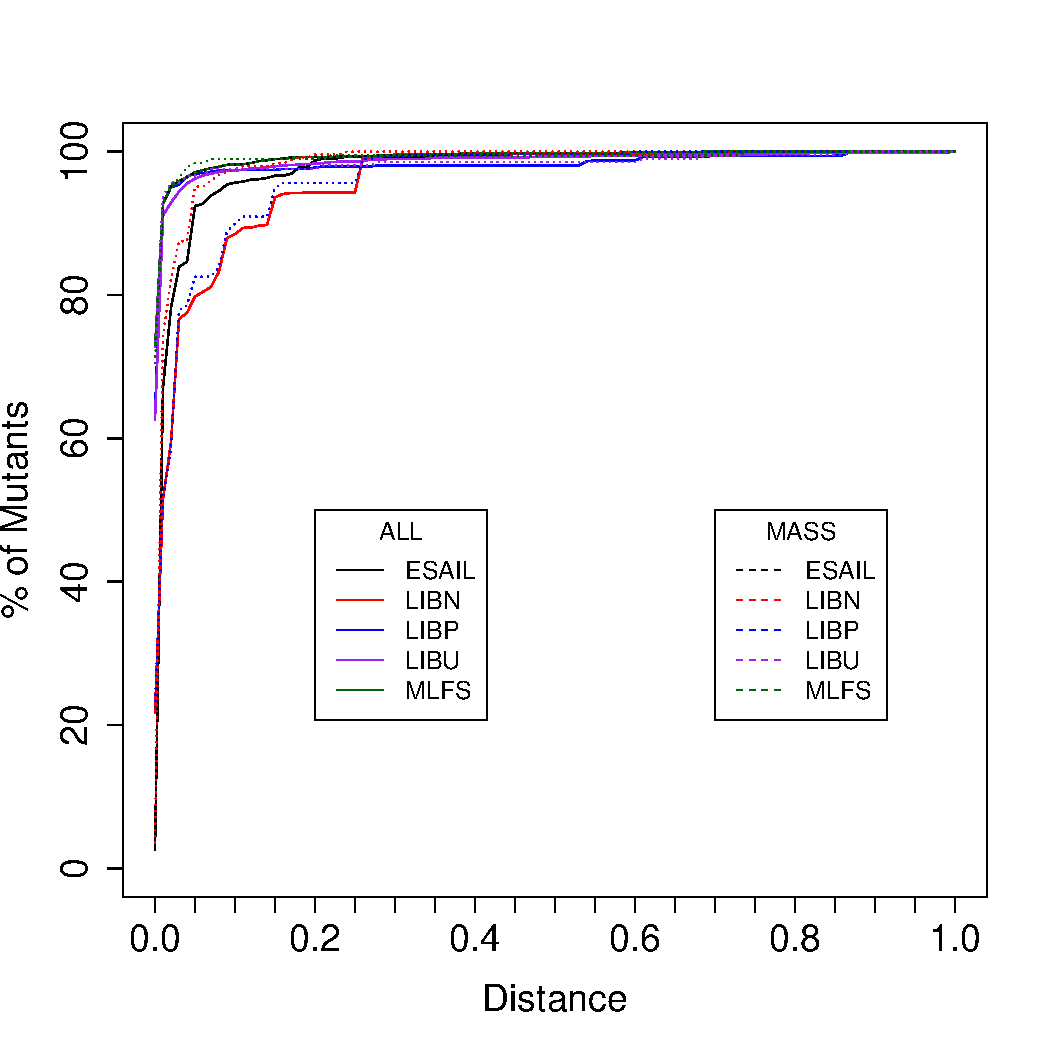
\includegraphics[width=0.6\columnwidth]{data/distanceFequency_Equivalent.pdf}
\caption{Cumulative distribution of mutants over distance values computed to determine equivalent mutants.}
\label{fig:results:test:dde}
\end{center}
\end{figure}

\begin{figure}[tb]
\begin{center}
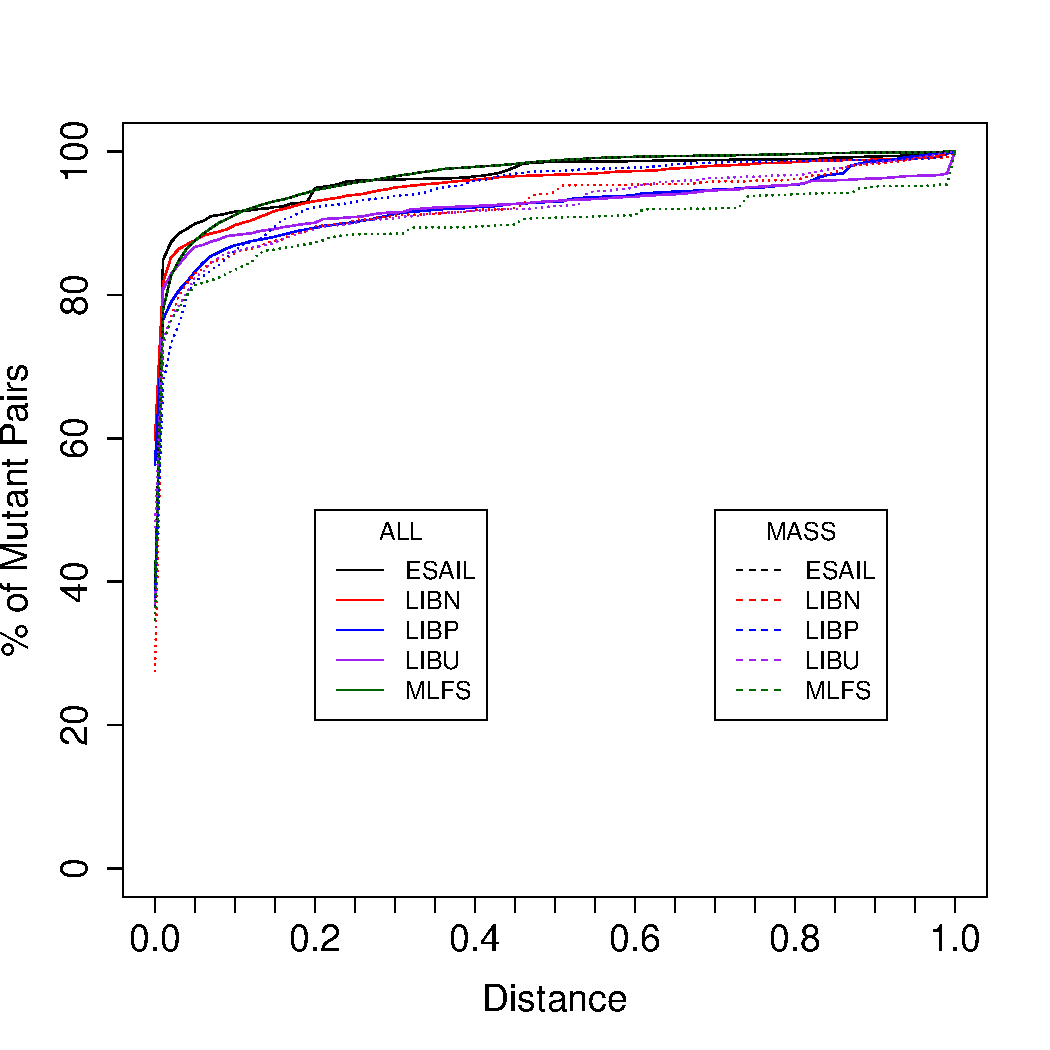
\includegraphics[width=0.6\columnwidth]{data/distanceFequency_Redundant.pdf}
\caption{Cumulative distribution of mutant pairs over distance values computed to determine duplicate mutants.}
\label{fig:results:test:ddd}
\end{center}
\end{figure}



We determine the values of $T_E$ and $T_D$ based on the analysis of the 
cumulative distribution of the distance values computed to determine equivalent and duplicate mutants, for the two configurations listed above.
Figures~\ref{fig:results:test:dde} and
~\ref{fig:results:test:ddd}
show the cumulative distribution --- the Y-axis shows the percentage of mutants and mutant pairs with a distance lower or equal to the value in the X-axis.
For both Figures~\ref{fig:results:test:dde} and
~\ref{fig:results:test:ddd} we can observe that the distribution of mutants is not uniform in the range 0-1 (otherwise we would have straight lines with 45 degree angle) but we observe a large proportion of mutants (Figures~\ref{fig:results:test:dde}) and mutant pairs (Figures~\ref{fig:results:test:ddd}) having small distances. For example,
Figure~\ref{fig:results:test:dde} shows that, across all subjects, more than 60\% of the mutants have a distance below 0.05 (i.e., with $x$ equal to $0.05$, the value of $y$ is above $60$). 
%Also, for \PARAM{}, \UTIL{}, and \MLFS{}{} more than half of the mutants have a distance equal to zero (i.e., all the test cases show the same coverage of the original program). 
%This observation, i.e., a large percentage of mutants with a small distance from the original program, should be expected since mutation operators introduce small changes into the source code which unlikely lead to big changes to the program behaviour.
%Figure~\ref{fig:results:test:ddd} shows a similar distribution for the distances computed for duplicate mutants.

To evaluate precision and recall, we thus select values for $T_D$ and $T_E$ that 
either largely differ (i.e., $0.0$, $0.4$, and $0.8$) or delimit ranges including a large proportion of the mutants (i.e., $0$, $0.01$, and $0.05$). Table~\ref{table:results:proportion:mutants} reports the percentage of mutants and mutant pairs belonging to the ranges delimited by the selected values, for the two configurations considered in our study; the distribution of mutants in Table~\ref{table:results:proportion:mutants} is consistent with Figures~\ref{fig:results:test:dde} and
~\ref{fig:results:test:ddd}.

% !TEX root =  ../Main.tex

% \begin{table}[h]
% \caption{RQ7. Precision of Coverage-Based Detection of Equivalent Mutants.}
% \label{table:results:precision:equivalent} 
% \tiny
% \begin{tabular}{|
% p{10mm}|p{10mm}|p{10mm}|
% p{3mm}|p{3mm}|p{3mm}|p{3mm}|p{3mm}|p{3mm}|p{3mm}|p{3mm}|p{3mm}|p{3mm}|
% p{3mm}|p{3mm}|p{3mm}|p{3mm}|p{3mm}|p{3mm}|p{3mm}|p{3mm}|p{3mm}|p{3mm}|
% |}
% \hline
% \textbf{Case Study}&\textbf{Operators}&\textbf{Sampling}&\multicolumn{9}{c|}{\textbf{Precision of equivalent mutants detection when distance $< T_E$.}}&\multicolumn{9}{c|}{\textbf{Precision of redundant mutants detection when distance $< T_R$.}}\\ 
% &&
% &\textbf{0.0}&\textbf{0.0}&\textbf{0.30}&\textbf{0.40}&\textbf{0.50}&\textbf{0.60}&\textbf{0.70}&\textbf{0.80}&\textbf{0.90}
% &\textbf{0.10}&\textbf{020}&\textbf{0.30}&\textbf{0.40}&\textbf{0.50}&\textbf{0.60}&\textbf{0.70}&\textbf{0.80}&\textbf{0.90}\\
% \hline
% \\
% $\mathit{\SAIL{}}_{S}$
% &All
% &None
% &0.01
% \\
% ..
% \\
% $\mathit{\SAIL{}}_{S}$
% &All
% &\FIXME{Random 1\%}
% &0.01
% \\
% ..
% \\
% $\mathit{\SAIL{}}_{S}$
% &SDL
% &\FIXME{Random 1\%}
% &0.01
% \\
% ..
% \\

% \end{tabular}

% \end{table}
% $(0-0.40]$,  $(0.40-0.80]$, and $(0.80-1.0]$



\begin{table}[h]
\caption{Distribution (\%) of mutants in distance ranges.}
\label{table:results:proportion:mutants} 
\scriptsize
\centering
\begin{tabular}{|
@{\hspace{1pt}}p{14mm}@{\hspace{1pt}}|
@{\hspace{1pt}}p{5mm}@{\hspace{1pt}}|
@{\hspace{1pt}}>{\raggedleft\arraybackslash}p{5mm}@{\hspace{1pt}}|
@{\hspace{1pt}}>{\raggedleft\arraybackslash}p{5mm}@{\hspace{1pt}}|
@{\hspace{1pt}}>{\raggedleft\arraybackslash}p{5mm}@{\hspace{1pt}}|
@{\hspace{1pt}}>{\raggedleft\arraybackslash}p{5mm}@{\hspace{1pt}}|
@{\hspace{1pt}}>{\raggedleft\arraybackslash}p{5mm}@{\hspace{1pt}}|
>{\raggedleft\arraybackslash}p{5mm}@{\hspace{1pt}}|
@{\hspace{1pt}}>{\raggedleft\arraybackslash}p{5mm}@{\hspace{1pt}}|
@{\hspace{1pt}}>{\raggedleft\arraybackslash}p{5mm}@{\hspace{1pt}}|
@{\hspace{1pt}}>{\raggedleft\arraybackslash}p{5mm}@{\hspace{1pt}}|
@{\hspace{1pt}}>{\raggedleft\arraybackslash}p{5mm}@{\hspace{1pt}}|
@{\hspace{1pt}}>{\raggedleft\arraybackslash}p{5mm}@{\hspace{1pt}}|
}
\hline
& \multicolumn{6}{c|}{\textbf{Distance for nonequivalent}}  & \multicolumn{6}{c|}{\textbf{Distance for nonduplicate}}  \\
\cline{2-13}
\textbf{}& (0.00 & (0.00 & (0.01& (0.05 & (0.4 & (0.8
& (0.00 & (0.00 & (0.01& (0.05 & (0.4 & (0.8\\
\textbf{Config.}& 0.00] & 0.01] & 0.05]& 0.40] & 0.8] & 1.0] 
& 0.00] & 0.01] & 0.05]& 0.40] & 0.8] & 1.0] \\
\hline
ALL   
& 53.9  & 29.8  & 10.1 & 5.5  & 0.5  & 0.2  
& 39.2  & 40.5  & 7.3 & 7.6  & 2.6  & 2.8  
\\
\APPR  
% & 25.3  & 47.7  &18.0  & 8.4 & 0.6  & 0.0 
% & 36.9  & 40.2  & 7.4 & 9.5  & 3.5  & 2.5 
& 39.7  & 36.7  & 16.4  & 6.6 & 0.4  & 0.1 
& 33.7  & 37.9  & 10.5 & 10.5  & 3.8  & 3.3 
\\
\hline
\end{tabular}
\end{table}




%\begin{table}[h]
%\caption{RQ7. Precision of Coverage-Based Detection of Nonequivalent/Nonduplicate Mutants (all mutants tested with the whole test suite).}
%\label{table:results:precision:equivalent} 
%\scriptsize
%\centering
%\begin{tabular}{|
%@{\hspace{1pt}}p{12mm}@{\hspace{1pt}}|
%@{\hspace{1pt}}p{5mm}@{\hspace{1pt}}|
%@{\hspace{1pt}}>{\raggedleft\arraybackslash}p{9mm}@{\hspace{1pt}}|
%@{\hspace{1pt}}>{\raggedleft\arraybackslash}p{9mm}@{\hspace{1pt}}|
%@{\hspace{1pt}}>{\raggedleft\arraybackslash}p{10mm}@{\hspace{1pt}}|
%>{\raggedleft\arraybackslash}p{5mm}@{\hspace{1pt}}|
%@{\hspace{1pt}}>{\raggedleft\arraybackslash}p{10mm}@{\hspace{1pt}}|
%@{\hspace{1pt}}>{\raggedleft\arraybackslash}p{10mm}@{\hspace{1pt}}|
%@{\hspace{1pt}}>{\raggedleft\arraybackslash}p{10mm}@{\hspace{1pt}}|
%}
%\hline
%& \multicolumn{4}{c|}{\textbf{Nonequivalent mutants ratio}}  & \multicolumn{4}{c|}{\textbf{Nonduplicate mutants ratio}}  \\
%\textbf{Distance} & 0.0 & 0-0.4 & 0.4-0.8 & 0.8-1.0 & 0.0 & 0-0.4 & 0.4-0.8 & 0.8-1.0 \\
%  \cline{0-0}
%  \textbf{Subject} &&&&&&&&\\
%\hline
%\PARAM{}   & 0.75 & 1& 1 & 1& 0.75& 1 & 1 & 1\\
%\GCSP{}   & 0.25 & 1& 1 & 1& 1   & 1& 1 & 1\\
%\UTIL{}    & 0.25 & 1& 1 & 1& 1   & 1& 1 & 1\\
%\MLFS{}{}	   & 0.25 & 1& 1 & -& 1   & 1& 1 & 1\\
%\SAIL{}$_S$  & 0.5  & 1& 1 & -& 1   & 1& 1 & 1\\
%\hline
%\textbf{Overall}      & 0.4 & 1& 1 & 1& 0.95& 1& 1 & 1 \\
%\hline
%\end{tabular}
%\end{table}
%
%\begin{table}[h]
%\caption{RQ7. RQ7. Precision of Coverage-Based Detection of Nonequivalent/Nonduplicate Mutants (mutants sampled with FSCI, tested with \APPR test suite).}
%\label{table:results:precision:equivalent:reduced} 
%\scriptsize
%\centering
%\begin{tabular}{|
%@{\hspace{1pt}}p{12mm}@{\hspace{1pt}}|
%@{\hspace{1pt}}p{5mm}@{\hspace{1pt}}|
%@{\hspace{1pt}}>{\raggedleft\arraybackslash}p{9mm}@{\hspace{1pt}}|
%@{\hspace{1pt}}>{\raggedleft\arraybackslash}p{9mm}@{\hspace{1pt}}|
%@{\hspace{1pt}}>{\raggedleft\arraybackslash}p{10mm}@{\hspace{1pt}}|
%>{\raggedleft\arraybackslash}p{5mm}@{\hspace{1pt}}|
%@{\hspace{1pt}}>{\raggedleft\arraybackslash}p{10mm}@{\hspace{1pt}}|
%@{\hspace{1pt}}>{\raggedleft\arraybackslash}p{10mm}@{\hspace{1pt}}|
%@{\hspace{1pt}}>{\raggedleft\arraybackslash}p{10mm}@{\hspace{1pt}}|
%}
%\hline
%& \multicolumn{4}{c|}{\textbf{Nonequivalent mutants ratio}}  & \multicolumn{4}{c|}{\textbf{Nonduplicate mutants ratio}}  \\
%\textbf{Distance} & 0.0 & 0-0.4 & 0.4-0.8 & 0.8-1.0 & 0.0 & 0-0.4 & 0.4-0.8 & 0.8-1.0 \\
%  \cline{0-0}
%  \textbf{Subject} &&&&&&&&\\
%\hline
%\PARAM{}   & 0.5  & 1   & 1 & -& 1   & 1 & 1 & 1\\
%\GCSP{}   & 0.0  & 0.75& - & -& 1   & 1& 1 & 1\\
%\UTIL{}    & 0.5   & 1   & 1 & -& 1   & 1& 1 & 1\\
%\MLFS{}{}	   & 0.0   & 1   & - & -& 1   & 1& 1 & -\\
%\SAIL{}$_S$  & 0.75     & 1   & 1 & -& 1   & 1& 1 & 1\\
%\hline
%Total      & 0.35   & 0.95& 1 & -& 1   & 1& 1 & 1 \\
%\hline
%\end{tabular}
%\end{table}
%



%, $0.4$,  and $0.8$.

%Indeed, in case the distance for mutants and mutant pairs is not uniformly distributed in the range [0;1], we would like to study values for $T_E$ and $T_D$ ha.





%To determine $T_E$, for each configuration listed above (i.e., ALL and FSCI/SMTS), we manually inspect a randomly selected subset of the mutants. However, 
To compute precision and recall for different values of $T_E$, since the distribution of mutants is not uniform, we rely on stratified sampling, as follows. 
%More precisely, we estimate precision and recall based on the number of nonequivalent mutants estimated for sets of mutants selected based on their distance, 
We divide all the live mutants into six buckets, based on their distance from the original program, according to the ranges reported in Table~\ref{table:results:proportion:mutants}. 
%More precisely, we considered mutants with a distance of 0 (i.e., having the same coverage as the original program), and within the ranges $(0-0.01]$, $(0.01-0.05]$, $(0.05-0.40]$,  $(0.40-0.80]$, and $(0.80-1.0]$.  
We determine the ratio ($r_R$) of nonequivalent mutants in a specific range $R$ by randomly selecting 20 mutants (four for each subject) and inspecting them with the help of the engineers who developed the software. 
We rely on $r_R$ to estimate $e_{R}$, that is, the number of nonequivalent mutants in the entire set of mutants with a distance within the specific  range $R$
$$e_R = r_R * n_R$$
with $n_R$ being the number of mutants observed in the range $R$ for all the subjects\footnote{$n_R$ can be derived from Table~\ref{table:results:proportion:mutants}}.
Based on $e_R$, we estimate the number of nonequivalent mutants above a threshold and, consequently, compute precision and recall. We perform the analysis for both selected configurations,  ALL and \APPR.

%Our aim is to identify a threshold value above which  we observe a high precision and recall; 
Our aim is to identify a threshold value above which  we
maximize the number of nonequivalent mutants being selected (high recall) and maximize the number of equivalent mutants being discarded (high precision); since both precision and recall are equally important, we look for a threshold value that maximizes the harmonic mean of precision and recall (F-value).
%90\% of the mutants are nonequivalent. 
%Note: In case a mutant is shared by multiple configurations we may assume it is resampled
%In total, we therefore manually inspected 240 mutants (20 mutants x 6 buckets x 2 configurations)
%In total, we manually inspected 240 mutants (20 mutants x 6 buckets x 2 configurations), a larger number than that considered in related studies~\cite{schuler2013covering}.

To determine $T_D$, we repeated the same procedure as for $T_E$, except that we considered both killed and live mutants according to the procedure indicated in Section 1.2.3.7 from D2.

In total, we manually inspected 410 mutants (186 mutants to detect equivalent mutants and 224 mutant pairs to detect duplicate ones), a larger number than that considered in related studies~\cite{schuler2013covering}. The number of inspected mutants is lower than the maximum of 480 (\{20 mutants + 20 mutant pairs\} x 6 buckets x 2 configurations) because the mutant distribution across ranges is not perfectly uniform (see Table~\ref{table:results:ratio:equivalent} for the number of observations per bucket).

%duplicate
%               [,1]         [,2]        [,3]        [,4]         [,5]
%  [1,] 36.496664796 59.844728918 56.30110509 36.88708075 39.133748088
%  [2,] 48.377106531 21.876953376 20.26347083 43.87784519 38.779706252
%  [3,]  2.501076925  3.528421173  2.43483919  2.17803086  4.725099324
%  [4,]  1.225083870  1.195644418  1.67758329  1.33416054  2.223305809
%  [5,]  0.633101414  0.625080276  1.17171310  1.34543443  1.680639400
%  [6,]  0.719581761  0.551726106  1.43394443  1.09352273  1.063168534
%  [7,]  0.351142846  0.663327197  1.18294605  0.27075425  0.919557014
%  [8,]  0.687600350  0.300837722  0.96874528  0.45398330  0.804628685
%  [9,]  0.164802172  0.250317535  0.53298421  0.32920228  0.754954614
% [10,]  0.229417677  0.338228368  0.54654122  0.44697948  0.515221811
% [11,]  0.244103019  0.576558063  0.41716860  0.13338894  0.572327436
% [12,]  0.136736852  0.341368041  0.26184399  0.14314911  0.591786373
% [13,]  0.065268187  0.291704129  0.31917078  0.10236878  0.317405579
% [14,]  0.175897764  0.475232264  0.19560830  0.30028327  0.397164406
% [15,]  0.069836960  0.413865936  0.18747410  0.18478797  0.326955778
% [16,]  0.201026016  0.470665468  0.24635026  0.12335766  0.303226957
% [17,]  0.058741368  0.241754792  0.28857066  0.26521897  0.214504633
% [18,]  0.425548579  0.292274978  0.25603384  0.14945255  0.295567241
% [19,]  0.093333507  0.331378174  0.29438081  0.19095585  0.383865836
% [20,]  0.067878914  0.269726420  0.17159303  0.15175703  0.260071793
% [21,]  2.014828932  0.206362118  0.24635026  0.11615050  0.404661149
% [22,]  0.143916352  0.168971472  0.22814513  0.52813345  0.149217780
% [23,]  0.158928035  0.178105065  0.12549919  0.05575947  0.245925765
% [24,]  0.258788361  0.167829773  0.12782325  0.05381647  0.188168249
% [25,]  0.357669665  0.251744659  0.15881070  0.10058394  0.228357310
% [26,]  0.077016461  0.122447232  0.14254229  0.07618352  0.212027449
% [27,]  0.017948751  0.129297427  0.20994000  0.08169621  0.125684526
% [28,]  0.049277481  0.256026031  0.13518277  0.23986965  0.164602400
% [29,]  0.062983800  0.228339827  0.29089472  0.16522245  0.212842312
% [30,]  0.025780934  0.158981604  0.19870705  0.10410844  0.170143471
% [31,]  0.037855548  0.251744659  0.30522642  0.04862009  0.187353386
% [32,]  0.015011683  0.112171940  0.15106384  0.04416927  0.194393805
% [33,]  0.035571162  0.145281215  0.12743590  0.39867569  0.135886615
% [34,]  0.031655071  0.093619329  0.07669395  0.02835419  0.202900979
% [35,]  0.010116569  0.129868276  0.11039280  0.11461418  0.141688443
% [36,]  0.019580456  0.071927045  0.10148391  0.08296142  0.148565889
% [37,]  0.035571162  0.111315666  0.08366613  0.04832638  0.203944004
% [38,]  0.017622410  0.125016055  0.04260775  0.04502781  0.098402900
% [39,]  0.060373073  0.106748869  0.03795963  0.03056830  0.048239911
% [40,]  0.029697025  0.090765081  0.08792690  0.04053180  0.069426359
% [41,]  0.187972379  0.103894621  0.09180033  0.04166145  0.088005244
% [42,]  0.077669143  0.109888542  0.06778506  0.07550573  0.069002630
% [43,]  0.183403605  0.107034294  0.06197491  0.03515467  0.077509804
% [44,]  0.206573812  0.142997817  0.06158756  0.07997914  0.064080855
% [45,]  0.351142846  0.070499922  0.22465904  0.02227668  0.112222983
% [46,]  0.440560262  0.055372408  0.05384070  0.09934132  0.078259478
% [47,]  0.497343585  0.041386594  0.07436989  0.06583594  0.119328592
% [48,]  0.080606211  0.047095089  0.04803055  0.08921967  0.130117383
% [49,]  0.081585234  0.031682151  0.07746863  0.11944907  0.075325970
% [50,]  0.058741368  0.036248947  0.06584834  0.05115050  0.076206022
% [51,]  0.014032660  0.045097116  0.05035461  0.05853841  0.102477217
% [52,]  0.011095592  0.044526266  0.03912166  0.09742092  0.073924405
% [53,]  0.021212161  0.035392673  0.35945447  0.05318387  0.051140825
% [54,]  0.006526819  0.033680124  0.05267867  0.06974452  0.038722307
% [55,]  0.010769251  0.017696337  0.15571196  0.02263816  0.110691040
% [56,]  0.002937068  0.062222603  0.02478996  0.04080292  0.046870941
% [57,]  0.014032660  0.064220576  0.05848882  0.06649113  0.047588021
% [58,]  0.025780934  0.125301480  0.03602292  0.10182655  0.030312917
% [59,]  0.002284387  0.060510054  0.06623568  0.06933785  0.034485018
% [60,]  0.002937068  0.026829930  0.03757229  0.04762600  0.022620607
% [61,]  0.037202867  0.044811691  0.10303328  0.03016163  0.050195584
% [62,]  0.011421933  0.027971629  0.24983635  0.14312652  0.015482404
% [63,]  0.017622410  0.039959470  0.04415712  0.03562913  0.015938727
% [64,]  0.009790228  0.056514107  0.07591926  0.07878171  0.027868327
% [65,]  0.003916091  0.167829773  0.05771413  0.05311609  0.019719694
% [66,]  0.025780934  0.082773187  0.04957993  0.03840806  0.019687099
% [67,]  0.003263409  0.035392673  0.05112930  0.09484532  0.019882666
% [68,]  0.008158523  0.105607170  0.04183306  0.10715849  0.009908739
% [69,]  0.041118958  0.067645674  0.07398255  0.12918665  0.015677971
% [70,]  0.011421933  0.093619329  0.05384070  0.19563260  0.006518907
% [71,]  0.003916091  0.063078877  0.05151664  0.02977755  0.007985661
% [72,]  0.012074615  0.040244894  0.05887616  0.04405631  0.029139514
% [73,]  0.026107275  0.039103195  0.03447354  0.05291275  0.009126470
% [74,]  0.004568773  0.059939205  0.06274959  0.03400243  0.019100397
% [75,]  0.005221455  0.031111301  0.12162576  0.28677267  0.018024778
% [76,]  0.020559479  0.136147622  0.02517731  0.06179179  0.016003917
% [77,]  0.002610727  0.063649727  0.01200764  0.03264685  0.035560637
% [78,]  0.014032660  0.017410912  0.11813967  0.11585679  0.019263370
% [79,]  0.006853160  0.027115354  0.11116749  0.05621133  0.012842247
% [80,]  0.017622410  0.029398753  0.06429897  0.01509211  0.028878758
% [81,]  0.016317047  0.081631488  0.08250410  0.11739311  0.047653210
% [82,]  0.007179501  0.090765081  0.12975996  0.14073166  0.008441984
% [83,]  0.022191184  0.023404832  0.42723952  0.31569168  0.031290753
% [84,]  0.012074615  0.070785346  0.48185491  0.06590372  0.041949166
% [85,]  0.115198350  0.030825877  0.29360613  0.04071255  0.019132992
% [86,]  0.041771640  0.013414965  0.11504092  0.01671880  0.019230775
% [87,]  0.028065320  0.018838036  0.13402074  0.05124087  0.017112131
% [88,]  0.029044343  0.009704443  1.06325701  0.03063608  0.018872236
% [89,]  0.051561868  0.025973655  0.29980362  0.08592110  0.024022172
% [90,]  0.029370684  0.021121434  0.21303875  0.05467501  0.014048244
% [91,]  0.023496547  0.011987841  0.10729406  0.03404762  0.004791397
% [92,]  0.044382367  0.016554637  0.12007638  0.03904067  0.003715777
% [93,]  0.029697025  0.021121434  0.04493181  0.09552311  0.014700135
% [94,]  0.027086298  0.007135620  0.21497546  0.09762426  0.002542374
% [95,]  0.020559479  0.025973655  0.22349701  0.09613312  0.003846155
% [96,]  0.055151618  0.118736710  0.09373705  0.02125999  0.002086050
% [97,]  0.031002389  0.067360249  0.13944354  0.06610705  0.004041722
% [98,]  0.228112313  0.072783320  0.12704856  0.02128259  0.045730132
% [99,]  0.066573551  0.140714418  0.16036007  0.02659194  0.013103003
%[100,]  0.014359001  0.373906466  0.03950900  0.21958115  0.013363759
%[101,]  0.162191445  0.280001713  0.17972723  3.05574546  0.009289442


%
% precision repeat the experiment 10 times for a total of 1000 mutants inspected. Finally we compute the percentage of equivalent mutants among the selected live mutants with difference above T\%, for values of T that var between 10\% and 90\%.
%
%We repeat the experiments considering two set of mutants, the complete set, and the set derived with SDL.

%schuler2013covering says: Coverage impact—the number of methods that have at least one statement that is executed at a different frequency in the mutated run than in the normal run—while leaving out the method that contains the mutation

% Oscar: We might study T as an element of experimentation, see how different thresholds impact on the correct classification of non-equivalent mutants.

%To answer this research question, for all live mutants we estimate the code coverage difference T\% with respect to the original version, those mutants with code coverage difference lower than T\% are then classified as equivalent mutants and get discarded.

%Then, for the X\% of the mutants with code coverage difference higher than T\% we try to generate inputs using the constraint solving tool KLEE. For each of these mutants, for which we are able to generate inputs, we classify them as a \textit{correct} non-equivalent, otherwise is classified as an \textit{incorrect} non-equivalent.

%To measure the \textit{effectiveness} of our approach, we estimate the precision and recall of our technique. The \textit{precision} is the percentage of mutants that are correctly classified as non-equivalent, that is, the mutant has a code coverage difference higher than T\% and is non-equivalent. The \textit{recall} is the percentage of non-equivalent mutations that are correctly classified as such.

\paragraph{Results}


The ratio ($r_R$) of nonequivalent mutants, for the distance ranges reported in Table~\ref{table:results:ratio:equivalent}, shows
similar results for both configurations (ALL and \APPR). 
The differences in distribution between mutants (Table~\ref{table:results:proportion:mutants}) and equivalent mutants  (Table~\ref{table:results:ratio:equivalent}), for both  configurations, is indeed not statistically significant and effect size is negligible.
%The differences between the two configurations is not statistically significant and effect size is negligible.
Such similarity suggests that nonequivalent and nonduplicate mutants follow the same distribution for both configurations. This can be explained since 
FSCI sampling uniformly selects 
%the mutants selected for \APPR using FSCI sampling are 
a subset of the mutants considered by the ALL configuration, which includes all mutants. 



The 14 nonequivalent mutants leading to $d=0$ across the two configurations (seven for ALL, seven for \APPR) have the following characteristics.
Four mutants (29\%) invalidate data buffers' preconditions (e.g., an array size is indicated as larger than it should be). Since such faults are typically detected through profiling (e.g., by using Valgrind~\cite{Valgrind}), not detecting such mutants cannot be considered a major weakness of the approach. Seven mutants (50\%) affect variables that are not used in the mutated source file (i.e., the one for which we collect code coverage). 
%Lightweight static analysis (e.g., searching for a keyword within the source code) should enable the identification of these mutants as nonequivalent. 
Static analysis should, in principle, enable the identification of these mutants as nonequivalent. 
Three mutants (21\%) concern the deletion of clauses that are not tested by our test suites; these cases might be detected by our approach after combining statement coverage with additional coverage measures (e.g., clause coverage) to compute distances, but this is left to future work. Based on the above, the percentage of nonequivalent mutants that
may potentially indicate limitations of the test suite, cannot easily be detected by other means, 
and are ignored with $T_E$, when set to zero, is very low 
 (i.e., three out of 160, or 1.88\%). For this reason, \textbf{we consider the proposed $T_E$ threshold precise enough to be used for test suite evaluation in a safety context}.
 
Table~\ref{table:results:precision:equivalent} provides precision and recall obtained for different $T_E$ values; more precisely, we report the results obtained when all mutants are considered nonequivalent (i.e., $d\ge0$), along with the results obtained for $T_E$ being set to $0$, $0.01$, $0.05$, $0.4$, and $0.8$. 

% !TEX root =  ../Main.tex

% \begin{table}[h]
% \caption{RQ7. Precision of Coverage-Based Detection of Equivalent Mutants.}
% \label{table:results:precision:equivalent} 
% \tiny
% \begin{tabular}{|
% p{10mm}|p{10mm}|p{10mm}|
% p{3mm}|p{3mm}|p{3mm}|p{3mm}|p{3mm}|p{3mm}|p{3mm}|p{3mm}|p{3mm}|p{3mm}|
% p{3mm}|p{3mm}|p{3mm}|p{3mm}|p{3mm}|p{3mm}|p{3mm}|p{3mm}|p{3mm}|p{3mm}|
% |}
% \hline
% \textbf{Case Study}&\textbf{Operators}&\textbf{Sampling}&\multicolumn{9}{c|}{\textbf{Precision of equivalent mutants detection when distance $< T_E$.}}&\multicolumn{9}{c|}{\textbf{Precision of redundant mutants detection when distance $< T_R$.}}\\ 
% &&
% &\textbf{0.0}&\textbf{0.0}&\textbf{0.30}&\textbf{0.40}&\textbf{0.50}&\textbf{0.60}&\textbf{0.70}&\textbf{0.80}&\textbf{0.90}
% &\textbf{0.10}&\textbf{020}&\textbf{0.30}&\textbf{0.40}&\textbf{0.50}&\textbf{0.60}&\textbf{0.70}&\textbf{0.80}&\textbf{0.90}\\
% \hline
% \\
% $\mathit{\SAIL{}}_{S}$
% &All
% &None
% &0.01
% \\
% ..
% \\
% $\mathit{\SAIL{}}_{S}$
% &All
% &\FIXME{Random 1\%}
% &0.01
% \\
% ..
% \\
% $\mathit{\SAIL{}}_{S}$
% &SDL
% &\FIXME{Random 1\%}
% &0.01
% \\
% ..
% \\

% \end{tabular}

% \end{table}
% $(0-0.40]$,  $(0.40-0.80]$, and $(0.80-1.0]$

\begin{table}[tb]
\caption{RQ6. Ratio ($r_R$) of Nonequivalent/Nonduplicate Mutants per Distance Range.}
\label{table:results:ratio:equivalent} 
\scriptsize
\centering
\begin{tabular}{|
@{\hspace{1pt}}p{10mm}@{\hspace{1pt}}|
@{\hspace{1pt}}p{5mm}@{\hspace{1pt}}|
@{\hspace{1pt}}>{\raggedleft\arraybackslash}p{5mm}@{\hspace{1pt}}|
@{\hspace{1pt}}>{\raggedleft\arraybackslash}p{5mm}@{\hspace{1pt}}|
@{\hspace{1pt}}>{\raggedleft\arraybackslash}p{5mm}@{\hspace{1pt}}|
@{\hspace{1pt}}>{\raggedleft\arraybackslash}p{5mm}@{\hspace{1pt}}|
@{\hspace{1pt}}>{\raggedleft\arraybackslash}p{5mm}@{\hspace{1pt}}|
>{\raggedleft\arraybackslash}p{5mm}@{\hspace{1pt}}|
@{\hspace{1pt}}>{\raggedleft\arraybackslash}p{5mm}@{\hspace{1pt}}|
@{\hspace{1pt}}>{\raggedleft\arraybackslash}p{5mm}@{\hspace{1pt}}|
@{\hspace{1pt}}>{\raggedleft\arraybackslash}p{5mm}@{\hspace{1pt}}|
@{\hspace{1pt}}>{\raggedleft\arraybackslash}p{5mm}@{\hspace{1pt}}|
@{\hspace{1pt}}>{\raggedleft\arraybackslash}p{4mm}@{\hspace{1pt}}|
}
\hline
& \multicolumn{6}{c|}{\textbf{Distance range (nonequivalent)}}  & \multicolumn{6}{c|}{\textbf{Distance range (nonduplicate)}}  \\
\textbf{}& (0.00 & (0.00 & (0.01& (0.05 & (0.4 & (0.8
& (0.00 & (0.00 & (0.01& (0.05 & (0.4 & (0.8\\
\textbf{Config.}& 0.00] & 0.01] & 0.05]& 0.40] & 0.8] & 1.0] 
& 0.00] & 0.01] & 0.05]& 0.40] & 0.8] & 1.0] \\
\hline
ALL   
& 0.35  & 0.85  & 1.00 & 1.00  & 1.00  & 1.00  
& 0.95  & 1.00  & 1.00 & 1.00  & 1.00  & 1.00  
\\
& (20)  & (20)  & (20) & (20)  & (18)  & (12)  
& (20)  & (20)  & (20) & (20)  & (20)  & (20)  
\\
\APPR  
& 0.35  & 0.95  & 1.00  & 1.00 & 1.00  & N/A
& 1.00  & 1.00 & 1.00 & 1.00  & 1.00  & 1.00
\\
& (20)  & (20)  & (20) & (10)  & (6)  & (0)  
& (20)  & (20)  & (20) & (20)  & (18)  & (16)  
\\
\hline
\end{tabular}

\textbf{Note}: We report the number of observations in parenthesis.
\end{table}


\begin{table}[tb]
\caption{RQ6. Precision (P), Recall (R), and their harmonic mean (F) obtained for the Coverage-Based Detection of Nonequivalent/Nonduplicate Mutants.}
\label{table:results:precision:equivalent} 
\scriptsize
\centering
\begin{tabular}{|
@{\hspace{1pt}}p{6mm}@{\hspace{1pt}}|
@{\hspace{1pt}}p{2mm}@{\hspace{1pt}}|
@{\hspace{1pt}}p{5mm}@{\hspace{1pt}}|
@{\hspace{1pt}}>{\raggedleft\arraybackslash}p{5mm}@{\hspace{1pt}}|
@{\hspace{1pt}}>{\raggedleft\arraybackslash}p{6mm}@{\hspace{1pt}}|
@{\hspace{1pt}}>{\raggedleft\arraybackslash}p{6mm}@{\hspace{1pt}}|
@{\hspace{1pt}}>{\raggedleft\arraybackslash}p{6mm}@{\hspace{1pt}}|
@{\hspace{1pt}}>{\raggedleft\arraybackslash}p{6mm}@{\hspace{1pt}}|
>{\raggedleft\arraybackslash}p{5mm}@{\hspace{1pt}}|
@{\hspace{1pt}}>{\raggedleft\arraybackslash}p{5mm}@{\hspace{1pt}}|
@{\hspace{1pt}}>{\raggedleft\arraybackslash}p{6mm}@{\hspace{1pt}}|
@{\hspace{1pt}}>{\raggedleft\arraybackslash}p{6mm}@{\hspace{1pt}}|
@{\hspace{1pt}}>{\raggedleft\arraybackslash}p{6mm}@{\hspace{1pt}}|
@{\hspace{1pt}}>{\raggedleft\arraybackslash}p{6mm}@{\hspace{1pt}}|
}
\hline
&& \multicolumn{6}{c|}{\textbf{Threshold (nonequivalent)}}  & 
\multicolumn{6}{c|}{\textbf{Threshold (nonduplicate)}}  \\
\cline{3-14}
\textbf{Conf.}&&\tiny{d $\ge$ 0}& \tiny{d\textgreater0} &\tiny{d\textgreater0.01}& \tiny{d\textgreater0.05}& \tiny{d\textgreater0.4} & \tiny{d\textgreater0.8}
&\tiny{d $\ge$ 0}& \tiny{d\textgreater0} &\tiny{d\textgreater0.01}& \tiny{d\textgreater0.05}& \tiny{d\textgreater0.4} & \tiny{d\textgreater0.8}
\\

\hline
\multirow{2}{*}{ALL}&P   
& 0.62  & 0.90  & 1.00 & 1.00  & 1.00  & 1.00  
& 0.98  & 1.00  & 1.00 & 1.00  & 1.00  & 1.00  \\
&R   
& 1.00  & 0.71  & 0.28 & 0.10  & 0.01  & 0.01
& 1.00  & 0.62  & 0.21 & 0.13  & 0.05  & 0.03  
\\
&F   
& 0.77  & \underline{0.80}  & 0.44 & 0.19  & 0.03  & 0.01
& \underline{0.99}  & 0.77  & 0.34 & 0.23  & 0.10  & 0.05  
\\
\hline
\multirow{1}{*}{\emph{MA}}&P 
& 0.81  & 0.97  & 1.00  & 1.00 & 1.00 & N/A 
& 1.00  & 1.00 & 1.00 & 1.00  & 1.00  & 1.00
\\
\multirow{1}{*}{\emph{SS}}&R
& 1.00  & 0.89  & 0.33  & 0.11 & 0.01  & N/A
& 1.00  & 0.63 & 0.22 & 0.16  & 0.06  & 0.02
\\
&F   
& 0.90  & \underline{0.93}  & 0.50 & 0.20  & 0.02  & N/A
& \underline{1.00}  & 0.77  & 0.37 & 0.27  & 0.11  & 0.05  
\\
\hline
\end{tabular}
\end{table}



%
%
%
%
%
%
%\begin{table}[h]
%\caption{RQ6. Precision (P) and Recall (R) of Coverage-Based Detection of Nonequivalent/Nonduplicate Mutants.}
%\label{table:results:precision:equivalent} 
%\scriptsize
%\centering
%\begin{tabular}{|
%@{\hspace{1pt}}p{5mm}@{\hspace{1pt}}|
%@{\hspace{1pt}}p{10mm}@{\hspace{1pt}}|
%@{\hspace{1pt}}p{5mm}@{\hspace{1pt}}|
%@{\hspace{1pt}}>{\raggedleft\arraybackslash}p{5mm}@{\hspace{1pt}}|
%@{\hspace{1pt}}>{\raggedleft\arraybackslash}p{5mm}@{\hspace{1pt}}|
%@{\hspace{1pt}}>{\raggedleft\arraybackslash}p{5mm}@{\hspace{1pt}}|
%@{\hspace{1pt}}>{\raggedleft\arraybackslash}p{5mm}@{\hspace{1pt}}|
%@{\hspace{1pt}}>{\raggedleft\arraybackslash}p{5mm}@{\hspace{1pt}}|
%>{\raggedleft\arraybackslash}p{5mm}@{\hspace{1pt}}|
%@{\hspace{1pt}}>{\raggedleft\arraybackslash}p{5mm}@{\hspace{1pt}}|
%@{\hspace{1pt}}>{\raggedleft\arraybackslash}p{5mm}@{\hspace{1pt}}|
%@{\hspace{1pt}}>{\raggedleft\arraybackslash}p{5mm}@{\hspace{1pt}}|
%@{\hspace{1pt}}>{\raggedleft\arraybackslash}p{5mm}@{\hspace{1pt}}|
%@{\hspace{1pt}}>{\raggedleft\arraybackslash}p{5mm}@{\hspace{1pt}}|
%}
%\hline
%&& \multicolumn{6}{c|}{\textbf{Nonequivalent mutants ratio}}  & \multicolumn{6}{c|}{\textbf{Nonduplicate mutants ratio}}  \\
%\cline{2-14}
%&\textbf{Distance}& 0.00 & 0.00 & 0.01& 0.05 & 0.4 & 0.8
%& 0.00 & 0.00 & 0.01& 0.05 & 0.4 & 0.8\\
%&\textbf{range}& 0.00 & 0.01 & 0.05& 0.40 & 0.8 & 1.0 
%& 0.00 & 0.01 & 0.05& 0.40 & 0.8 & 1.0 \\
%\hline
%\multirow{2}{*}{$r_R$}&ALL   
%& 0.35  & ?  & ? & 1  & 1  & 1  
%& 0.95  & ?  & ? & 1  & 1  & 1  
%\\
%&SMTS  
%& 0.35  & ?  & ?  & 0.95 & 1  & 1
%& 0.35  & ? & ? & 1  & 1  & 1
%\\
%\hline
%\multirow{2}{*}{P}&ALL   
%& 0.35  & ?  & ? & 1  & 1  & 1  
%& 0.95  & ?  & ? & 1  & 1  & 1  
%\\
%&SMTS  
%& 0.35  & ?  & ?  & 0.95 & 1  & 1
%& 0.35  & ? & ? & 1  & 1  & 1
%\\
%\hline
%\multirow{2}{*}{R}&ALL   
%& 0.35  & ?  & ? & 1  & 1  & 1  
%& 0.95  & ?  & ? & 1  & 1  & 1  
%\\
%&SMTS  
%& 0.35  & ?  & ?  & 0.95 & 1  & 1
%& 0.35  & ? & ? & 1  & 1  & 1
%\\
%\hline
%\end{tabular}
%\end{table}



%\begin{table}[h]
%\caption{RQ7. Precision of Coverage-Based Detection of Nonequivalent/Nonduplicate Mutants (all mutants tested with the whole test suite).}
%\label{table:results:precision:equivalent} 
%\scriptsize
%\centering
%\begin{tabular}{|
%@{\hspace{1pt}}p{12mm}@{\hspace{1pt}}|
%@{\hspace{1pt}}p{5mm}@{\hspace{1pt}}|
%@{\hspace{1pt}}>{\raggedleft\arraybackslash}p{9mm}@{\hspace{1pt}}|
%@{\hspace{1pt}}>{\raggedleft\arraybackslash}p{9mm}@{\hspace{1pt}}|
%@{\hspace{1pt}}>{\raggedleft\arraybackslash}p{10mm}@{\hspace{1pt}}|
%>{\raggedleft\arraybackslash}p{5mm}@{\hspace{1pt}}|
%@{\hspace{1pt}}>{\raggedleft\arraybackslash}p{10mm}@{\hspace{1pt}}|
%@{\hspace{1pt}}>{\raggedleft\arraybackslash}p{10mm}@{\hspace{1pt}}|
%@{\hspace{1pt}}>{\raggedleft\arraybackslash}p{10mm}@{\hspace{1pt}}|
%}
%\hline
%& \multicolumn{4}{c|}{\textbf{Nonequivalent mutants ratio}}  & \multicolumn{4}{c|}{\textbf{Nonduplicate mutants ratio}}  \\
%\textbf{Distance} & 0.0 & 0-0.4 & 0.4-0.8 & 0.8-1.0 & 0.0 & 0-0.4 & 0.4-0.8 & 0.8-1.0 \\
%  \cline{0-0}
%  \textbf{Subject} &&&&&&&&\\
%\hline
%\PARAM{}   & 0.75 & 1& 1 & 1& 0.75& 1 & 1 & 1\\
%\GCSP{}   & 0.25 & 1& 1 & 1& 1   & 1& 1 & 1\\
%\UTIL{}    & 0.25 & 1& 1 & 1& 1   & 1& 1 & 1\\
%\MLFS{}{}	   & 0.25 & 1& 1 & -& 1   & 1& 1 & 1\\
%\SAIL{}$_S$  & 0.5  & 1& 1 & -& 1   & 1& 1 & 1\\
%\hline
%\textbf{Overall}      & 0.4 & 1& 1 & 1& 0.95& 1& 1 & 1 \\
%\hline
%\end{tabular}
%\end{table}
%
%\begin{table}[h]
%\caption{RQ7. RQ7. Precision of Coverage-Based Detection of Nonequivalent/Nonduplicate Mutants (mutants sampled with FSCI, tested with \APPR test suite).}
%\label{table:results:precision:equivalent:reduced} 
%\scriptsize
%\centering
%\begin{tabular}{|
%@{\hspace{1pt}}p{12mm}@{\hspace{1pt}}|
%@{\hspace{1pt}}p{5mm}@{\hspace{1pt}}|
%@{\hspace{1pt}}>{\raggedleft\arraybackslash}p{9mm}@{\hspace{1pt}}|
%@{\hspace{1pt}}>{\raggedleft\arraybackslash}p{9mm}@{\hspace{1pt}}|
%@{\hspace{1pt}}>{\raggedleft\arraybackslash}p{10mm}@{\hspace{1pt}}|
%>{\raggedleft\arraybackslash}p{5mm}@{\hspace{1pt}}|
%@{\hspace{1pt}}>{\raggedleft\arraybackslash}p{10mm}@{\hspace{1pt}}|
%@{\hspace{1pt}}>{\raggedleft\arraybackslash}p{10mm}@{\hspace{1pt}}|
%@{\hspace{1pt}}>{\raggedleft\arraybackslash}p{10mm}@{\hspace{1pt}}|
%}
%\hline
%& \multicolumn{4}{c|}{\textbf{Nonequivalent mutants ratio}}  & \multicolumn{4}{c|}{\textbf{Nonduplicate mutants ratio}}  \\
%\textbf{Distance} & 0.0 & 0-0.4 & 0.4-0.8 & 0.8-1.0 & 0.0 & 0-0.4 & 0.4-0.8 & 0.8-1.0 \\
%  \cline{0-0}
%  \textbf{Subject} &&&&&&&&\\
%\hline
%\PARAM{}   & 0.5  & 1   & 1 & -& 1   & 1 & 1 & 1\\
%\GCSP{}   & 0.0  & 0.75& - & -& 1   & 1& 1 & 1\\
%\UTIL{}    & 0.5   & 1   & 1 & -& 1   & 1& 1 & 1\\
%\MLFS{}{}	   & 0.0   & 1   & - & -& 1   & 1& 1 & -\\
%\SAIL{}$_S$  & 0.75     & 1   & 1 & -& 1   & 1& 1 & 1\\
%\hline
%Total      & 0.35   & 0.95& 1 & -& 1   & 1& 1 & 1 \\
%\hline
%\end{tabular}
%\end{table}
%



 We can observe that \textbf{$T_E$ set to zero enables the accurate detection of nonequivalent mutants}. Indeed, 
for $d>0$, we achieve the highest F-value, and the highest precision and recall, given that a value of $1.00$ cannot be achieved simultaneously for precision and recall.
These results are in line with related work~\cite{zhang2013faster} reporting that a difference in the frequency of execution of a single line of code (i.e., $d>0$) is indicative of a mutant not being equivalent to the original software.
Moreover, these results also indicate that \textbf{FSCI mutants sampling and \MPTS selection enable the accurate identification of nonequivalent mutants based on $T_E$}.



As for duplicate mutants, based on Table~\ref{table:results:precision:equivalent}, 
mutants are highly likely to be nonduplicate and thus \textbf{it is not possible to determine a threshold to identify duplicate mutants}. Indeed, among all the considered threshold values, the highest F-value is obtained when all the mutants are considered nonduplicate (i.e., $d\ge0$). These results are in line with related work~\cite{shin2017theoretical} showing that test suites are unlikely to distinguish nonredundant mutants (i.e., many nonduplicate and nonsubsumed mutants yield the same test results). 
%SHin et al show that 60,043 out of 242,437 mutants are detected as nonredundant.
With test suites that do not distinguish nonredundant mutants, it is very likely that nonduplicate mutants show the same coverage in addition to showing the same results. This is the reason why in Table~\ref{table:results:ratio:equivalent}, we observe a large percentage of nonduplicate mutants having the same coverage (i.e., $d=0$). For this reason, when no methods are available to automatically generate test cases that distinguish subsumed mutants (see Section~1.2.2 from D2), we suggest that all mutants should be considered as nonduplicate when computing the mutation score:

\begin{equation}
\label{equation:ms:exp}
\mathit{MS} = \frac{\mathit{KND}}{\mathit{LNE}+\mathit{KND}}
\end{equation}

where $\mathit{LNE}$ is the number of live, nonequivalent mutants.







\subsection{RQ7 - \APPR Mutation Score}

\paragraph{Design and measurements}

% Describe what it the purpose of the RQ
\JMR{3.16}{RQ7 investigates the extent to which  the mutation score estimated by MASS with Equation~\ref{equation:ms:exp}},
%RQ7 investigates the extent to which \APPR's mutation score estimate (i.e., the mutation score computed with Equation~\ref{equation:ms:exp}), 
%when relying on FSCI and a reduced and prioritized test suite, 
can accurately predict
the actual mutation score of the system.

% an over- or under- approximation of the mutation score computed with a  non-optimized mutation testing process (i.e., no mutants sampling and no test suite reduction/prioritization). 

To this end, we apply \APPR to the five subjects  described in Section~\ref{sec:empirical:subjects} and compute the mutation score according to equation~\ref{equation:ms:exp}.
\REVOCT{C-P-11}{We compare the resulting mutation scores with those obtained with a traditional, non-optimized mutation analysis process that tests all the mutants with the entire test suite and do not discard likely equivalent mutants. Being the non-optimized mutation analysis process our base truth.}
Since we have already demonstrated that FSCI, applied to a reduced and prioritized test suite, accurately estimates the mutation score (see RQ4), 
we discuss the percentage of live mutants that are discarded by means of $T_E$ and the effect it has on the mutation score.
%If the percentage of equivalent mutant discarded matches the one observed for RQ6 (i.e., 65\%), whose correctness was manually verified, we can conclude that \APPR enables the accurate estimation of the mutation score.



% Describe what we measure (ideally the same measurement of the referred papers)

\paragraph{Results}
From Table~\ref{table:results:mutationScore}, one can see that, on average, the percentage of live mutants that are discarded because considered equivalent is 42.28\%, which is in line with related work (i.e., 45\%~\cite{zhang2013faster}). Across our subjects, such percentage varies from 2.61\% (\SAIL{}$_S$) to 69.37\% (\MLFS{}{}), because of nondeterminism.
%based on the nondeterministic nature of the system. 
Indeed, complex embedded software, even when generating consistent functional results across multiple runs, may show nondeterminism 
in their nonfunctional properties (e.g., number of tasks started) 
%when the test environment is not well isolated (e.g., multiple test suites are run in parallel thus affecting performance).
when it is not possible to control the resources provisioned by the test environment.
For example, in our environment, \SAIL{}$_S$, which is a system including real-time tasks, show different code coverage for multiple executions of a same test case. The same happens for \GCSP{}, a network library, which may execute 
a different set of instructions
%different number of functions 
based on the current network usage (e.g., ports available on the host OS). 
%For such systems, the removal of equivalent mutants based on code coverage appears to be less effective. 
Unsurprisingly, in our experiments, the subject having the largest number of predicted equivalent mutants removed is the mathematical library \MLFS{}{}, which should not be affected by nondeterministic behaviour due to real-time constraints or networking. 

To maximize the number of equivalent mutants detected by \APPR, it is therefore advisable to minimize the sources of nondeterminism. It can be achieved, for example, by executing test cases in a dedicated testing environment, which is standard practice for space software. However, since our analysis concerned the execution of a large, entire set of mutants, not only a sampled subset, we relied on a shared HPC environment. This may have introduced unexpected delays in the execution of the simulator and altered the number of available ports, thus exacerbating nondeterminism.

As expected, the removal of equivalent mutants results in the \APPR mutation score being higher than that computed with a traditional approach. On average, the score increased by 10.52 percentage points (i.e., from $70.62\%$ to $81.14\%$). 

To provide some additional insights about the software features that, according to \APPR mutation analysis results, 
warrant to be verified with additional test cases, we report on the characteristics of
manually inspected mutants having $d > 0$ in Table~\ref{table:results:ratio:equivalent}.
%56 in total, I do want explain why, thus I do not put the number
According to our analysis, live mutants concern (1) logging functions (11\%),  (2) code developed by third parties (5\%), (3) time operations (e.g., timeouts, 4\%), (4) thread synchronisations (e.g., mutex locks, 5\%), (5) memory operations (e.g., malloc and free operations, 20\%), and (6) the application logic (55\%). Most of these categories either do not need to be tested (cases 1 and 2), or concern operations that are difficult to test (cases 3, 4, and 5) and often verified by other means, e.g., test suites including hardware in the loop or through manual inspection. However, most of the live mutants concerning the application logic have enabled engineers to identify weaknesses  in test suites
(e.g., corner cases not being tested, scenarios testable with simulators but verified only by test suites with hardware in the loop), 
which further stresses the importance of mutation analysis in this context.
Furthermore, the manual inspection of these live mutants led to the identification of 
one previously undetected bug
\JMR{3.15} {since the test suite was not covering a specific combination of boolean clauses in a function, a problem that may occur even when MC/DC adequacy is achieved by test suites~\cite{Gay2016}.}


% enable us to characterize the type of functions presenting live, nonequivalent mutants.
%based on the characteristics of the mutated source code: 
%(1) code that is executed with nondeterministic frequency (e.g., port opening closing), \FIXME{(2) functionalities writing to standard output,
%The main reasons for these mutants to not be killed are the following: 
%(1) the mutants are covered by other test suites (e.g., Unit test suite for $\SAIL{}\emph{-CSW}$ or hardware in the loop test suite for ONE case studies), 
%(2) \FIXME{return values of functions not propagated through the code, 
%(3) missing verification of corner cases and specific inputs, 
%(4) missing verification of final variables and final array’s values, 
%(5) missing verification of the negated condition on if and while closures, 
%(6) missing verification of variable values after iteration loops, and 
%(7) missing verification of time deltas between specific instructions}.
%
%These results indicate that, to be used as an acceptance criterion the mutation score should be computed by relying on all the software test suites.
 
% !TEX root =  ../Main.tex

\begin{table}[htb]
\caption{RQ7. \APPR Mutation Score.}
\label{table:results:mutationScore} 
\small
\centering
\begin{tabular}{|
>{\raggedleft\arraybackslash}p{24mm}@{\hspace{1pt}}|
>{\raggedleft\arraybackslash}p{46mm}@{\hspace{1pt}}|
>{\raggedleft\arraybackslash}p{25mm}@{\hspace{1pt}}|
>{\raggedleft\arraybackslash}p{25mm}@{\hspace{1pt}}|
}
\hline
\textbf{Subject}&\textbf{Predicted Equivalent}&\multicolumn{2}{c|}{\textbf{Mutation Score (\%)}}\\
&\textbf{Mutants Removed (\%)}&\textbf{Traditional}&\textbf{\APPR}\\ 
\hline
% 1225-32=1193; 2311/(2311+1193)
\SAIL{}$_{S}$&2.61&65.36&65.95\\
%$\mathit{\SAIL{}}$&&\\
% 4198-2281=1917; 10376/(10376+1917)


% 1214-770=444; 2717/(2717+444)

% 1712-371=1341; 3270/(3270+1341)
\GCSP{}&21.67&65.64&70.92\\
\PARAM{}&63.43&69.12&85.95\\
% 3981-2699=1282; 17484/(17484+1282)
\UTIL{}&54.34&71.20&84.41\\
\MLFS{}{}&69.37&81.80&93.49\\
\hline
$\textbf{Average}$&42.28&70.62&81.14\\
\hline
\end{tabular}

\end{table}

%2021-06-14
%Average MS with reduced test suite, above is with the whole TS
% 
%CSP 70.92
%LIBUTIL 84.41
%PARAM 85.95
%MLFS 93.49
%ESAIL 65.95





\clearpage
\subsection{RQ8 - Threshold for the mutation score}
\label{sec:exp:thr}
\paragraph{Design and measurements}


RQ8 aims to determine if it is possible to identify a threshold for the mutation score that ensures that the fault revealing power of a test suite is greater than the one of a test suite that simply achieves statement coverage adequacy (i.e., all the statements are covered).


We may perform an experiment in line with the one performed in reference [78]. The objective of the experiment would be to identify a mutation score that ensures that the fault revealing power of a test suite is greater than the one of a test suite that simply achieves statement coverage adequacy (i.e., all the statements are covered). 

Related work~\cite{CChekam:17} identify a threshold for the mutation score that ensures that a test suite with a mutation score above the given threshold detects all the mutants detected by a test suite that achieves statements coverage adequacy. 
We may perform an experiment in line with the one performed in reference~\cite{CChekam:17}.
To replicate such study, for every case study system, we may consider the original test suite, $\mathit{TS}_o$, which achieves 100\% coverage of non dead code, and an extended test suite, $\mathit{TS}_e$, that consists of the same test cases of $\mathit{TS}_o$ plus a set of test cases automatically generated to kill the mutants. The extended test suite achieves a mutation score $ms_e$ that is greater than the mutation score $\mathit{ms}_o$ of the original test suite. For example, we may have $\mathit{ms}_o=0.7$ and $\mathit{ms}_e=0.9$.

The experiment can be conducted by dividing the interval between $m_o$ and $m_i$ into $n$ ranges (e.g., 4 ranges), such that we can define $\delta = (\mathit{ms}_e - \mathit{ms}_o)/n$ and have each of the $n$ ranges defined as the interval between $\mathit{ms}_o+(n-1)*\delta$ and $\mathit{ms}_o+n*\delta$.
For every case study, for each of the $n$ ranges, we can generate $M$ test suites  (e.g., 10) by randomly selecting test cases belonging to $\mathit{TS}_i$ till we achieve a mutation score in the given range.
For each i-th test suite belonging to the range $n$ (i.e., $\mathit{TS}_{n,i}$), we compute the mutation score (i.e., $ms_{n,i}$).
Also, we compute the \INDEX{mutation score delta} as $msd_{n,i}=ms_{n,i}-ms_o$. Each test suite in the range $n$ enable us to study the fault revealing power of a test suite with a mutation score above the threshold $T=(n-1)*\delta$.

For each range $n$ we can perform a one sample t-test to reject the null hypothesis $msd_{n} = 0$ in favor of the alternate hypothesis $msd_{n} > 0$, at a 5\% alpha level.
If the null hypothesis is rejected in favor of the alternate hypothesis then the threshold $T=(n-1)*\delta$ ensures to achieve better fault detection than statement coverage adequacy.
Alternatively, we may perform a one sample wilcoxon-signed-rank test, which evaluates whether the median of the sample is greater than zero.

\REVNOV{PTCR-7}{Unfortunately, contrary to what we wrote in the previous version of report D2, such experiment would be of little value in our context because \APPR require the test suite to achieve a maximal statements coverage. Consequently, any test suite $\mathit{TS}_e$ would have a better mutation score than $\mathit{TS}_o$. Also, based on our assumption, it makes no sense to select a test suite $\mathit{TS}_e$ that does not achieve the same statement coverage of $\mathit{TS}_o$.}

\REVNOV{PTCR-7}{For this reason, the experiment should be performed with a set of real faults affecting the case study system not mutants. 
More precisely, for each i-th test suite belonging to the range $n$ (i.e., $\mathit{TS}_{n,i}$), we should compute the fault detection rate (i.e., $fdr_{n,i}$) as the proportion of real faults detected by the test suite. Similarly to what indicated above, we may compute the \INDEX{fault detection rate delta} as $fdrd_{n,i}=fdr_{n,i}-fdr_o$. Each test suite in the range $n$ enable us to study the fault revealing power of a test suite with a mutation score above the threshold $T=(n-1)*\delta$.}

\REVNOV{PTCR-7}{For each range $n$ we can perform a one sample t-test to reject the null hypothesis $fdr_{n} = 0$ in favor of the alternate hypothesis $fdr_{n} > 0$, at a 5\% alpha level.
If the null hypothesis is rejected in favor of the alternate hypothesis then the threshold $T=(n-1)*\delta$ ensures to achieve better fault detection than statement coverage adequacy.
Alternatively, we may perform a one sample wilcoxon-signed-rank test, which evaluates whether the median of the sample is greater than zero.}

\REVNOV{PTCR-7}{Despite such experiment would be of great value, the required information is not currently available and thus it is not possible at this stage of the project to commit for addressing this research question.}
\REVOCT{C-P-12}{Such problematics will be assessed on the FAQAS follow-on activity.}

\clearpage
\subsection{RQ9 - Combined mutation analysis results}
\label{sec:exp:thr}

\STARTCHANGEDWPT
\paragraph{Design and measurements}


RQ9 aims to determine whether is possible to combine results of mutation analysis for different test suites targeting the same system.

In CPSs, it is a common practice to verify and validate a system with different types of test suites. For example, it might be common to have a unit test suite verifying isolated components of a system, and then having a system test suite verifying complex use case scenarios of certain functionalities.

To answer this research question, we verify whether the mutation analysis results of an additional test suite can further improve the existing mutation score. We say that if the additional test suite is able to kill additional mutants, with respect to the existing test suite, then we conclude that mutation results from two test suites can be actually be combined.

In our experiments, in addition to the assessment of the ESAIL$_s$ system test suite, we also analyzed the ESAIL$_s$ unit test suite with the 3\,536 mutants previously generated.

\paragraph{Results}

The mutation score of the unit test suite is 26.78\%; there are 947 killed mutants, and 2\,589 live mutants. 

In addition to the set of 2\,311 mutants killed by the system test suite, we observe that the unit test suite kills 184 additional mutants. 
The result of mutation analysis combined for both test suites produce a mutation score of 70.56\% (an improvement of +4,8\%), which indicates that mutation analysis results can effectively be combined for different test suites (e.g., system and units).

\ENDCHANGEDWPT

\subsection{Discussion}
\label{sec:emp:discussion}

\JMR{2.3}{Our results show that the \APPR pipeline helps to overcome mutation analysis limitations caused by common  characteristics of embedded software, present in space systems and, more generally, in similar CPS (e.g., avionics, automotive, and industry 4.0).}

\JMRCHANGE{Although the need for dedicated hardware and simulators prevent the applicability of optimizations that make use of multi-threading or other OS functions to minimize mutants compilation time~\cite{untch1993mutation}, we have shown that our selective compilation strategy (see Section~1.2.7 from D2) is sufficient to achieve an efficient mutant compilation process (see Section~\ref{experimnt:setup}).}

\REVNOV{PTCR-PABG-27}{Trivial compiler optimization approaches are useful to eliminate a large proportion of mutants that are equivalent or duplicate. Based on our results, the presence of functions to deal with signals and data transformation does not limit the effectiveness of trivial compiler optimization approaches, which, across our subjects, enable the removal of 33,38\% of the mutants (62,351 out of 184,503). Our results are in line with empirical studies in the literature~\cite{papadakis2015trivial}. However, we show that for pure mathematical software (i.e., \MLFS{}{}), their effectiveness is significantly lower (i.e., 21\%, 6,717 out of 31,526).}

\REVNOV{PTCR-PABG-27}{The FSCI sampling approach with a confidence interval of 10\% is the most accurate approach for the estimation of the mutation score.} 
\REVNOV{PTCR-PABG-26}{We rely on a confidence interval of 10\% because it ensures that the deviation between the estimated and the actual mutation score is within +/- 5\%, in line with the choice made in related work (i.e., +/- 7\%~\cite{gopinath2015hard}). Comparison with other work is complicated by the use of a different evaluation strategy and statistics (for each case study, they consider subset of mutation adequate test suites, which is not feasible in our context)~\cite{zhang2013operator}.}
\REVNOV{PTCR-PABG-27}{Also, combined with test suite reduction and prioritization it saves, on average more than 80\% of the execution time; in other words, the mutation testing process takes only 20\% of the time required if all the mutants are executed with all the test cases that cover them. Similarly, the number of test cases being executed is reduced by more than 80\%.}

\REVNOV{PTCR-PABG-27}{The proposed approach for test suite reduction and prioritization reduces the time required for executing a test suite (e.g., when all the mutants are tested, in our case studies it reduce execution time up to 16.81\%). However, it contributes to a minimal reduction of execution time of compared with mutant sampling. Since test suite reduction and prioritization requires the monitoring of code coverage during mutation testing, which might be complicate for some systems, it might be avoided it practice without much loss in terms of performance.}

\REVNOV{PTCR-PABG-27}{When test suite reduction and prioritization is in place, the distance measures to be adopted are either $D_C$ and $D_E$.}

\JMRCHANGE{The time required to perform a traditional mutation analysis process that does not rely on mutants sampling (Step 5 of \APPR) is particularly high. Indeed it takes between 13 and 70 hours for unit and integration test suites and 11,001 hours for the system level test suite of \SAIL{}$_S$. These numbers confirm that the thorough testing required by critical CPS software, combined with long test execution times, may exacerbate the scalability problems of mutation analysis. 
\APPR applies FSCI-based mutation sampling and executes a prioritized subset of the test suite to address scalability issues. Our results show that such an optimized solution helps address scalability problems to a significant extent by reducing mutation analysis time by more than 70\% across subjects. In practice, for large software systems like \SAIL{}\emph{-CSW}, such reduction can make mutation analysis practically feasible; indeed, with 100 HPC nodes available for computation, \APPR can perform the mutation analysis of \SAIL{}\emph{-CSW} in half a day. In contrast, a traditional mutation analysis approach would take more than 100 days, thus largely delaying the development and quality assurance processes. Last, we demonstrated that FSCI-based sampling, a contribution of this paper, outperforms state-of-the-art mutants sampling strategies~\cite{zhang2013operator,gopinath2015hard} both in terms of mutation score accuracy and size of the selected mutant set.}

\JMRCHANGE{Finally, we confirm that a coverage-based approach (\APPR Step 7) enables the accurate identification of equivalent mutants, thus confirming related work's results~\cite{zhang2013faster} in our context. In addition, we demonstrate that such an approach still provides accurate results  
in the presence of optimizations (i.e., test suite reduction) that may affect the code coverage achieved by mutants. 
Coverage-based approaches, instead, are not effective in detecting likely duplicate mutants.}

\JMR{3.1}{This evaluation focused on investigating and identifying practical solutions to address the scalability of mutation analysis and the pertinence of mutation scores as an adequacy criterion in the context of embedded software for CPS. Important work remains concerning specific subjects in embedded software. For example, our work does not aim to assess if test suites can detect faults concerning the communication between heterogeneous components or the interoperability of different technologies and tools, two typical CPS problems. To address such issues, our future work includes the definition of mutation operators that alter the data exchanged by software components instead of their implementation.}
%Table~\ref{table:results:mutationScore} provides the results...
%
%% !TEX root =  ../Main.tex

\begin{table}[htb]
\caption{RQ7. \APPR Mutation Score.}
\label{table:results:mutationScore} 
\small
\centering
\begin{tabular}{|
>{\raggedleft\arraybackslash}p{24mm}@{\hspace{1pt}}|
>{\raggedleft\arraybackslash}p{46mm}@{\hspace{1pt}}|
>{\raggedleft\arraybackslash}p{25mm}@{\hspace{1pt}}|
>{\raggedleft\arraybackslash}p{25mm}@{\hspace{1pt}}|
}
\hline
\textbf{Subject}&\textbf{Predicted Equivalent}&\multicolumn{2}{c|}{\textbf{Mutation Score (\%)}}\\
&\textbf{Mutants Removed (\%)}&\textbf{Traditional}&\textbf{\APPR}\\ 
\hline
% 1225-32=1193; 2311/(2311+1193)
\SAIL{}$_{S}$&2.61&65.36&65.95\\
%$\mathit{\SAIL{}}$&&\\
% 4198-2281=1917; 10376/(10376+1917)


% 1214-770=444; 2717/(2717+444)

% 1712-371=1341; 3270/(3270+1341)
\GCSP{}&21.67&65.64&70.92\\
\PARAM{}&63.43&69.12&85.95\\
% 3981-2699=1282; 17484/(17484+1282)
\UTIL{}&54.34&71.20&84.41\\
\MLFS{}{}&69.37&81.80&93.49\\
\hline
$\textbf{Average}$&42.28&70.62&81.14\\
\hline
\end{tabular}

\end{table}

%2021-06-14
%Average MS with reduced test suite, above is with the whole TS
% 
%CSP 70.92
%LIBUTIL 84.41
%PARAM 85.95
%MLFS 93.49
%ESAIL 65.95

%
%\FIXME{Points to discuss}
%\begin{itemize}
%\item the portion of killed mutants that are removed because of redundancy is on average 13\%~\cite{gopinath2016limits}
%\item 40\% of mutants are equivalent~\cite{grun2009impact}
%\item the mutation score of a reduced test suite is an under-approximation of the real mutation score~\cite{Kurtz2016}
%\end{itemize}


\clearpage

%%NOTES
%In their study, Zhang et al. \cite{zhang2013operator} consider eight strategies for sampling mutants. In this paper, we consider two strategies. The first is the baseline sampling strategy, which consists of randomly selecting $r\%$ mutants from the complete mutants set. The second is the method-based sampling strategy, which is the best strategy according to Zhang et al. and consists of sampling mutants \textit{evenly across all functions of the SUT}, i.e., to sample $r\%$ mutants from each set of mutants generated inside a same function. Consider the set of mutants generated from the set of functions in the SUT as $M_{f_1}, M_{f_2}, ..., M_{f_n}$, then the set of sampled mutants can be defined as:
%
%\begin{equation}
% 	 M_{functions} = \cup_{i=1}^n Sample (M_{f_i}, r\%)
% \end{equation}
%
%%Similarly to Zhang et al., we rely on the sufficient set of mutation operators for generating the complete set of mutants. 
%
%%\TODO{In the background section we have to explain what "the sufficient set of mutation operators" is. To me it is not clear if you are referring to the original or the updated one.}
%
%%Fabrizio: can we reduce the min and max based on their results?
%
%%Similarly to Zhang et al. we consider different sampling ratios, between $5\%$ and $95\%$, in steps of $5\%$. 
%Differently from Zhang et al. we only consider sampling ratios ranging from $1\%$ to $10\%$, in steps of $1\%$. The reason is because for some of the software under analysis (e.g., the ESAIL system test suite), even considering a sampling ratio of $10\%$ means executing 6\,000 mutants for a test suite that finishes in 10 hours, which is more than 60\,000 hours of computation, a clearly infeasible scenario. 
%
%%More precisely, we consider $5\%, 10\%, 15\%, \ldots, 95\%$ of all the mutants generated.
%%F: 10 è il minimo per mann withnes
%
%
%
%
%To this end we study the confidence interval of the difference between the reduced set of mutants and the one for all the mutants.
%%To this end we study the confidence interval of the mean of the two population of mutants.
%Particularly, a confidence interval indicates that the estimated parameter (i.e., the mutation score for the sampled mutants), has a probability of $p_c$ (confidence level) of lying in it. We use a confidence level $p_c = 95\%$ in our experiments. 
%We compute the confidence interval using the Student's t method.
%
%%Here we should describe the mothod used to compute the CI. See my TOSEM'19 paper as a reference. 
%%Ideally, the two confidence intervals should be small and overlap.
%Ideally, the margin of error of the confidence interval should be small. In a previous study \cite{gopinath2015hard}, a pessimistic expected margin of error for the mutation score of sampled mutants has been statistically demonstrated to be $\pm 7\%$, thus, we expect the experimental error to be lower than this value.
%
%% In previous research~\cite{offutt1996experimental} it has been empirically demonstrated that the margin of error should be less than 1\%, to assure that a mutation score for the sampled mutants correctly estimates the one obtained with all the mutation operators.
%
%We repeat our comparison for the different sets of mutants generated with different p\% of mutants.
%
% %\TODO{Clopper-Pearson exact method, which I believe has to be used when using samples greater than 5\%, I need to study a bit more how to calculate the confidence interval}. 
%
%In addition, to compare with Zhang et al., we also use a linear regression model to determine how well the sampling mutation score predicts the selected mutation score for varying mutation score values. More precisely, we calculate the adjusted coefficient of determination $R^2$ to determine.
%
%%Our null hypothesis is that the mean is the same between mutation scores obtained with p\% of mutants and mutation scores obtained with all the available mutants.
%
%
%\TODO{(1) They calculate the $R^2$ coefficient for each triple ($P$, $S$, $r$), where P is the subject program, S the sampling strategy, and r the sampling ratio. For each triple, they generate a test suite, which is then used to calculate the mutation score of the sampled mutants and the selected mutants. This is repeated 20 times to obtain sampling and selected mutation scores for multiple samples. The $R^2$ coefficient is then estimated for all the generated test suites. A value close to 1, means that the sampled mutation score was a good predictor of the selected mutation score.}
%
%\TODO{(2) Also, they want to assess whether sampling mutation can be used for comparison of testing techniques and test suites, i.e., if a test suite T has a higher sampling mutation score than another test suite T', does T have a higher selected mutation score than T'? For this, they use the Kendall's $\tau$ and Spearman's $\rho$ rank correlation coefficients, which measure the strength of the agreement between two rankings.}




%\TODO{Oscar: i.e., for large software, running the 5\% of all the generated mutants can mean analyzing over 100\,000 for a 2MLOC program --which is still a very high number-- considering complex systems with test suites employing several hours to finish (e.g., ESAIL system test suite can take up to 10 hours).}

%Describe what we measure (ideally the same measurement of the referred papers)


%Consistently with RQ1 we adopt the strategy that sample mutants \textit{evenly across all functions of the SUT.} Also, similar to the work done by Gopinath et al.~\cite{gopinath2015hard} we also generate mutants with the \textit{sufficient} set of operators.

%Since the idea is to demonstrate that the representativeness of the mutation score obtained with random sampling does not depend from the proportion of mutants, but from a fixed number of mutants, we sample our subjects with both 100 and 1\,000 randomly sampled mutants independently from the size of the SUT. For each fixed number, we repeat the experiment 100 times to account for randomness (similar to the design by Gopinath et al.~\cite{gopinath2015hard}).
%
%Similar to RQ1, we again account for studying the \textit{representativeness} of the mutation score by means of a confidence interval. 
%More precisely, we study the confidence interval of the difference between the mutation score generated by the reduced set of mutants (i.e., generated with 100 and 1\,000 sampled mutants) and the mutation score generated with all the mutants. 
%As stated before, to account for representativeness of these sampling approaches, the margin of error should be kept lower than 1\%.
%
%\TODO{Oscar: First experiment, for one program, they sampled 1\,000 mutants and calculate the mutation score (repeated 100\,000 times), then the mean distribution was plotted along with the 2.5\% and 97.5\% quantiles. The idea is that theoretically the error should not be higher than 7\% when mutation sampling is used (experimentally was 3.1\%).
%In the second experiment they considered our procedure, that is, the mean absolute difference between the true mutation score and the sampled one (100 and 1\,000 mutants), were the mean and the error was estimated as a confidence interval at 95\%.}

%Describe what it the purpose of the RQ

%This research questions assesses if generating mutants with the statement deletion operator can lead to a mutation score that is representative of the mutation score of the whole suite.

%Describe what we measure (ideally the same measurement of the referred papers)

%Delamaro et al.~\cite{delamaro2014experimental} in his \textit{one-operator mutation experiment} studied the effectiveness of mutation testing by using a single operator, in terms of the mutation score and cost of the operator. Their results show that the statement deletion (SDL) operator presents the best trade-off between mutation score achieved, number of generated mutants, number of equivalent mutants and test cases necessary to kill all the mutants.

%Our goal is to determine if the mutants generated through the SDL operator enable us to compute a mutation score that is close to the one computed with all the available mutation operators.
%Similarly to previous research questions, the true mutation score is estimated by considering all the mutants generated by the \textit{sufficient} set of operators.

%We assess the \textit{representativeness} of one-operator mutation by comparing how close is the mutation score obtained with the SDL operator to the true mutation score, and how it compares to the mutation scores obtained with the random mutant selection approaches studied in RQ1 and RQ2.

% test suite prioritization strategy.
%The first strategy ($S_1$) consists of prioritizing test cases based on the number of times they cover the mutated statement~\cite{zhang2013faster}.
%The second strategy ($S_2$) matches the first strategy but, in addition, for every mutant, executes first those test cases that killed other mutants on the same line.
%The third strategy ($S_3$) consists of selecting and prioritizing test cases to maximize coverage diversity, 
%more specifically this strategy first select the single test case that cover the mutation more,
%and then iteratively, select test cases with the most different coverage profile (see Section~\ref{}).
%
%%presented above, in terms of execution time with respect to a non-prioritized test suite.
%
%%Describe what we measure (ideally the same measurement of the referred papers)

%For each subject $P$, strategy $S_i$ ($S_1, S_2$) and sampling ratio $r\%$ we estimate the mutation score and compare it to the true mutation score. For each 3-tuple (i.e., $P, S, r$), we repeat the experiment 10 times to account for randomness.
%Then, to assess for \textit{representativeness}, we study the confidence interval of the difference between the mutation score obtained through a reduced/prioritized test suite (e.g., for each 3-tuple $P, S, r$), and the one obtained using a non-optimized version of the test suite. 
%Ideally, the error margin of the confidence interval should be kept small to account for representativeness.


\ENDCHANGEDNOV